\documentclass[12pt]{article}
\usepackage{graphicx} % Required for inserting images
\usepackage{titling}  % For title size customization
\usepackage{hyperref} % For clickable links
\usepackage{tocloft}  % Optional: for customizing the TOC
\usepackage{amsmath}
\usepackage{tcolorbox}
\usepackage{tikz}
\renewcommand{\cftsecleader}{\cftdotfill{\cftdotsep}}
\usepackage[utf8]{inputenc}
\usepackage[T1]{fontenc}
\usepackage{graphicx} % Required for inserting images
\usepackage{tabularx}

\usepackage{amsmath, amssymb, amsthm} %nové matematika
\usepackage{graphicx, float}
\graphicspath{{img/}}

\usepackage[letterpaper, top=2.5cm, bottom=2cm]{geometry}

\title{\Huge Maturitní otázky z matematiky}
\author{
Michaela Dudašková, Aneta Foralová, Marek Fuchs, Oliver Hadraba, \\
Matiáš Horejsek, Marek Kalenda, Jonáš Lavička, Jan Peroutka, \\
Kateřina Polášková, Jakub Sláma, Roman Šnajder, Jakub Švagr
}


\date{April 2025}

\begin{document}

\maketitle

\tableofcontents % Adds the clickable table of contents
\listoffigures
\listoftables
\newpage         % Starts the main content on a new page

%\include{0.Předmluva}
\title{1. Rovnice a nerovnice s absolutní hodnotou a odmocninou mocninou}
\author{Jakub Sláma (Marek Fuchs)}
\date{24.4.2025}

\maketitle



\section{Rovnice a nerovnice s absolutní hodnotou a odmocninou mocninou}

\subsection{Absolutní hodnota}
\subsubsection{Absolutní hodnota reálného čísla} 
Absolutní hodnotu reálného čísla $a$, kde $a\in\mathbb{R}$ označujeme $|a|$ a platí pro ni:
\begin{equation}
|a|=\left\{
        \begin{matrix}         
            a, & \mbox{pokud }a \ge 0\\ 
            -a, &\mbox{pokud }a < 0
         \end{matrix}\right.
\end{equation}
\\
Pro kladnou hodnotu platí: $|1|= 1$, pro zápornou hodnotu platí: $|-1| = -(-1) = 1$

\subsubsection{Geometrický význam}
Absolutní hodnota nám vyjadřuje vzdálenost obrazu tohoto čísla od počátku
    \begin{figure}[H]
        \centering
        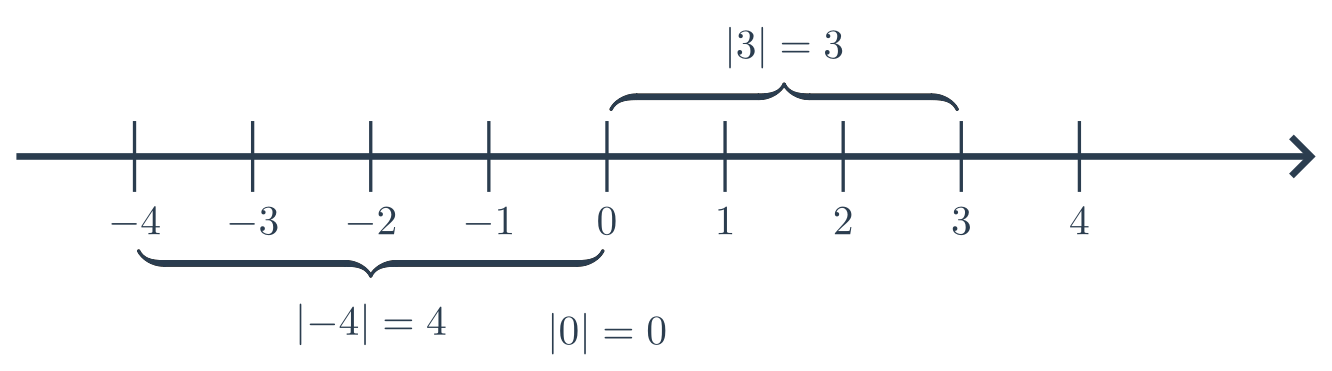
\includegraphics[width=0.5\linewidth]{img/ilustrace-absolutni-hodnota.png}
        \caption{Absolutní hodnota}
        \label{fig:enter-label}
    \end{figure}
\subsection{Mocnina a odmocnina z reálného čísla}
\textbf{Definice mocniny: }Pro libovolná reálná čísla $a$ a přirozená čísla $n$, kde:

\begin{itemize}
    \item $a$ je základ mocniny (říkáme mu základ nebo číslo, které umocňujeme)
    \item $n$ je exponent nebo mocnitel (říkáme mu stupeň nebo mocnina)
\end{itemize}
platí, že $a^n = a \cdot a \cdot a...$, tudíž: $a^3=a \cdot a \cdot a$
\subsubsection{Sudé mocniny, odmocniny}
Sudé mocniny jsou $a^x$, kde $x$ náleží celé sudé číslo např. $a^2; a^4; a^6$. Platí pro ně, že po umocnění čísla sudou mocninou bude výsledek vždy kladný.

Sudá odmocnina $\sqrt[x]{a}=n$, z nezáporného reálného čísla $a$ je takové nezáporné číslo $x$, pro které platí: $n^x = a; n\in\mathbb{R}^++\{0\}$.  Zapisujeme $\sqrt{a} = x$. Symbol $\sqrt{}$ se nazývá \textbf{odmocnítko}. Praxe: $\sqrt[2]{9}=3; \sqrt[2]{-9}=$ nelze v $\mathbb{R}$ (lze v $\mathbb{C}$).
\subsubsection{Liché mocniny, odmocniny}
Liché mocniny jsou $a^x$, kde $x$ náleží celé liché číslo např. $a^1; a^3; a^5$. Platí, že po umocnění čísla lichou mocninou bude výsledek se stejným znaménkem, jako základ.

Lichá odmocnina $\sqrt[x]{a}$, kde x náleží celému lichému číslu a $a \in\mathbb{R}$, platí: z reálného čísla \textbf{a} je reálné číslo \textbf{b}, pro které platí, že $b\cdot b \cdot b=a$ značíme $b=\sqrt[3]{a}$ Praxe: $\sqrt[3]{27}=3; \sqrt[3]{-27}=-3$. 


\subsubsection{Základní pravidla, pro počítání s mocninami a odmocninami}
Pro libovolné číslo $x \in \mathbb{R}$ a čísla $a,b,c,d \in \mathbb{Z}; b \land d\neq 0$ platí 
$$
    \sqrt[a]{x^b}=x^{\frac{b}{a}}, 
$$
$$
    x^\frac{a}{b} \cdot x^\frac{c}{d}=x^\frac{ad+cb}{bd}, \\
$$
$$
    (x^a)^b=x^{a \cdot b},
$$
$$
    \sqrt[a]{\sqrt[b]{x}} = \sqrt[a\cdot b]{x}.
$$
Přičemž číselný výsledek obecně $\in \mathbb{C}.$
\subsection{Ekvivalentní a důsledkové úpravy rovnic a nerovnic - rozdíly}
Při úpravách nerovnic používáme ekvivalentní úpravy, které se vyznačují tím, že nezmění platnost nerovnice. Smyslem ekvivalentních úprav je dostat nerovnici do jednoduššího tvaru. Výsledek rovnice s = je kořen/kořeny. Výsledek nerovnice je interval. Příklady rovnice a nerovnice:
$$
    3x+2=1+x
$$
$$
    |x+3| < 0
$$
\subsubsection{Ekvivalentní úpravy rovnic a nerovnic}
Ekvivalentní úpravy jsou takové, při kterých se nezmění počet výsledků rovnice, nebo nerovnice
\begin{itemize}
    \item přičtení výrazu 
    $$
        x-2=-2 /+2
    $$
    $$
        x-2+2=-2+2
    $$
    $$
        x=0
    $$
    \item odečtení výrazu
    $$
        x+2=2 /-2
    $$
    $$
        x+2-2=2-2
    $$
    $$
        x=0
    $$
    \item Vynásobení výrazem
    $$
        0,5x=3 / \cdot 2
    $$
    $$
        0,5x \cdot 2 = 3\cdot2
    $$
    $$
        x=6
    $$
    \item Vydělení výrazem
    $$
        3x=3 / \div3
    $$
    $$
        3x \div 3=3 \div 3
    $$
    $$
    x=1
    $$
    \end{itemize}
    Pokud násobíme nerovnici záporným číslem, potom musíme změnit znaménko nerovnosti.
    $$
        -x<1 / \cdot (-1)
    $$
    $$
        x>-1
    $$
\subsubsection{Důsledkové úpravy rovnic a nerovnic}
U důsledkových úprav (umocnění) získáme větší množství kořenů rovnice/nerovnice, tudíš musíme na konci výpočtu provést zkoužku (dosazení do původní rovnice/nerovnice a porovnání rovnosti pravé a levé strany), tímto způsobem vyřadíme nadbytečné nespávné výsledky.
\subsubsection{Rozdíly}

\begin{tabularx}{0.8\textwidth} { 
  | >{\raggedright\arraybackslash}X 
  | >{\centering\arraybackslash}X 
  | >{\raggedleft\arraybackslash}X | }
 \hline
 & Rovnice & Nerovnice\\
 \hline
 znaménko      &   $=$           & $\leq;<;>;\ge$\\
 násobení $-1$ &   nic se nemění & změna znaménka \\
 výsledek      &   n počet kořenů ($\mathbb{C}$) & interval \\
\hline
\end{tabularx}
\title{2. Lineární a mocninné funkce}
\author{Jakub Sláma}
\date{25.4.2025}

\maketitle

\section{Lineární a mocninné funkce}

\subsection{Lineární funkce}
\textbf{Definice funkce:} Množina sdružených číselných dvojic, pro které platí, že hodnota každého jednoho $x$ z definičního oboru náleží právě jedno $y$ z oboru hodnot. \\ \\ 
Předpis funkce: $f: y=f(x)$ \\
Grafem funkce $f$ je množina všech bodů roviny, které mají souřadnice $[x;f(x)]$  \\ \\
\textbf{lineární funkce:}
Grafem lineární funkce je přímka. $D(f) \in R$. 
Lineární funkcí rozumíme takovou, která má předpis:
$$
    f:y=kx+q
$$
$$
    k,q \in \mathbb{R}  
$$
kde $k$ je směrnice, jejíž hodnota udává strmost stoupání/klesání přímky a $q$ udává průsečík přímky s osami x a y. A pro hodnoty k platí: \\


\begin{tabularx}{0.8\textwidth} { 
  | >{\raggedright\arraybackslash}X 
  | >{\centering\arraybackslash}X 
  | >{\raggedleft\arraybackslash}X | }
 \hline
  k & co se děje s funkcí & viz.\\
 \hline
 $k>0$      &   funkce je rostoucí  & Figure 2\\
 $k=0$      &   konstantní         & Figure 3\\
 $k<0$      &   klesající          & Figure 4\\
\hline
\end{tabularx}


\begin{figure}[H]
        \centering
        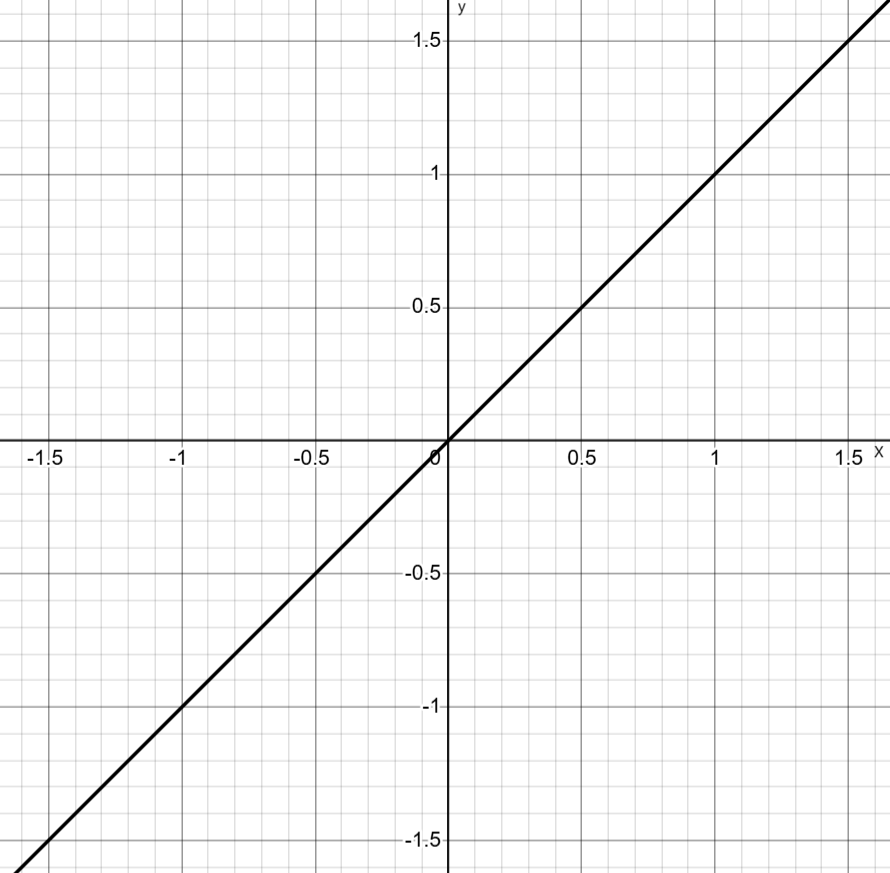
\includegraphics[width=0.4\linewidth]{img/2_graf_y=x.png}
        \caption{$f(x):$ $y=x$}
        \label{fig:enter-label}
    \end{figure}

\begin{figure}[H]
        \centering
        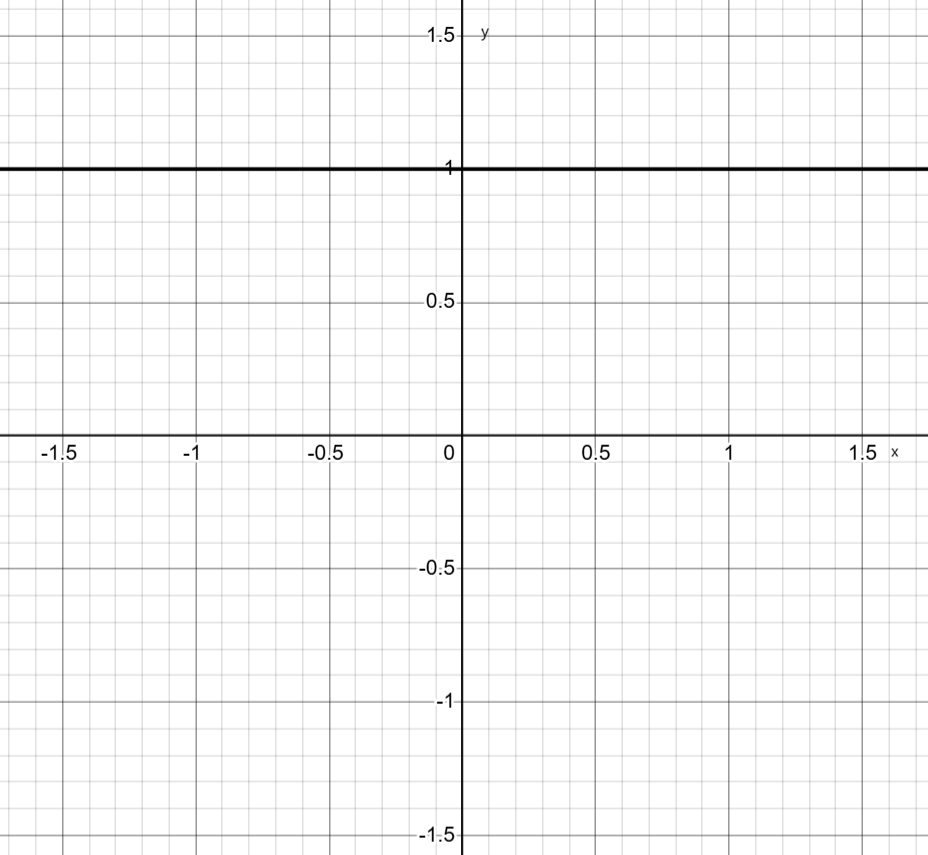
\includegraphics[width=0.4\linewidth]{img/2_graf_y=0x+1.png}
        \caption{$f(x):$ $y=0x+1$}
        \label{fig:enter-label}
    \end{figure}

\begin{figure}[H]
        \centering
        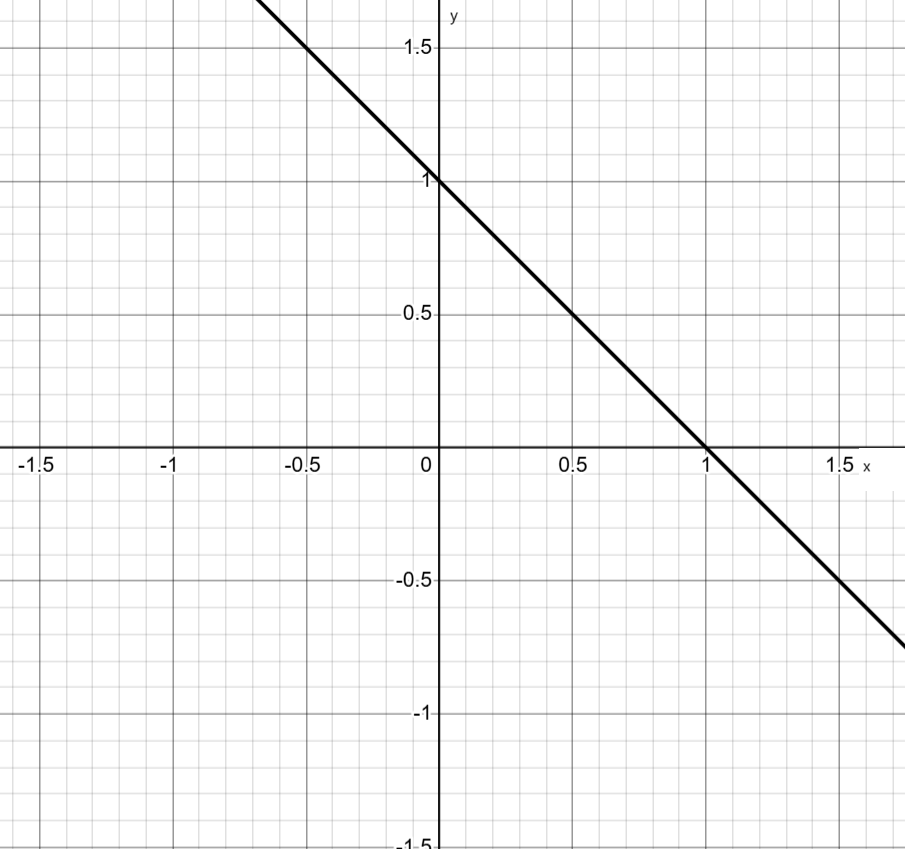
\includegraphics[width=0.4\linewidth]{img/2_graf_y=-x+1.png}
        \caption{$f(x):$ $y=-x+1$}
        \label{fig:enter-label}
    \end{figure}

\subsection{Mocninná funkce pro $n \in \mathbb{N}$ (celá čísla)}
Mocninná funkce má předpis: $y=x^n$, kde $n \in \mathbb{N}$. Vlastnosti se liší pro sudá a lichá $n$
Pro předpis$y=x^n$, kde $n \in \mathbb{N}$ a platí: \\

\begin{tabularx}{0.8\textwidth} { 
  | >{\centering\arraybackslash}X 
  | >{\centering\arraybackslash}X 
  | >{\raggedleft\arraybackslash}X | }
 \hline
  \textbf{sudá funkce} & \textbf{lichá funkce}\\
 \hline
 $n$ je sudé      &   $n$ je liché  \\
 \hline
 $D(f)=\mathbb{R}$      &   $D(f) = \mathbb{R}$         \\
 \hline
 $H(f)=\langle0;\infty)$      &   $H(f) = \mathbb{R}$         \\
 \hline
 je sudá      &   je lichá          \\
 \hline
 Je omezená z dola, shora omezená není      &   není shora ani zdola omezená          \\
 \hline
 není prostá *     &   je prostá          \\
 \hline
 klesající na $(-\infty;0\rangle$ a rostoucí na $\langle0;\infty)$      &      je rostoucí v $\mathbb{R}$       \\
 \hline
 má v bodě 0 minimum $f(0) = 0$      &           nemá maximum, ani minimum  \\
\hline
nemá maximum $f(0) = 0$      &             \\
\hline
viz. Figure 5     &    viz. Figure 6         \\
\hline
\end{tabularx} \\ \\
 *(Prostá funkce je v funkce, která žádnou funkční hodnotu nenabývá vícekrát)

\begin{figure}[H]
        \centering
        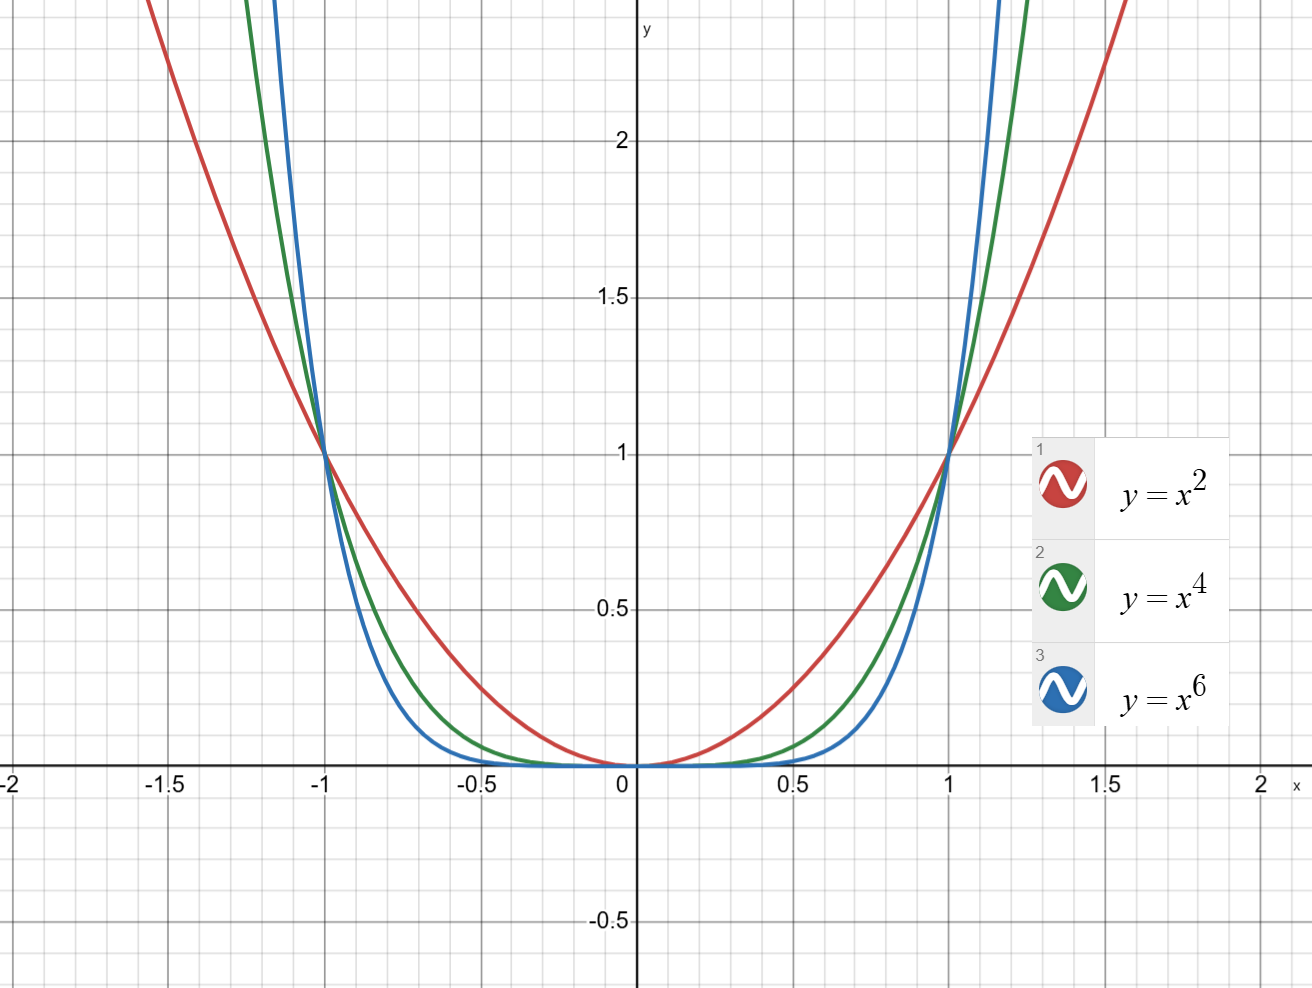
\includegraphics[width=0.5\linewidth]{img/2_sude_fkce.png}
        \caption{grafy funkcí s sudými mocninami} 
        \label{fig:enter-label}
    \end{figure}

\begin{figure}[H]
        \centering
        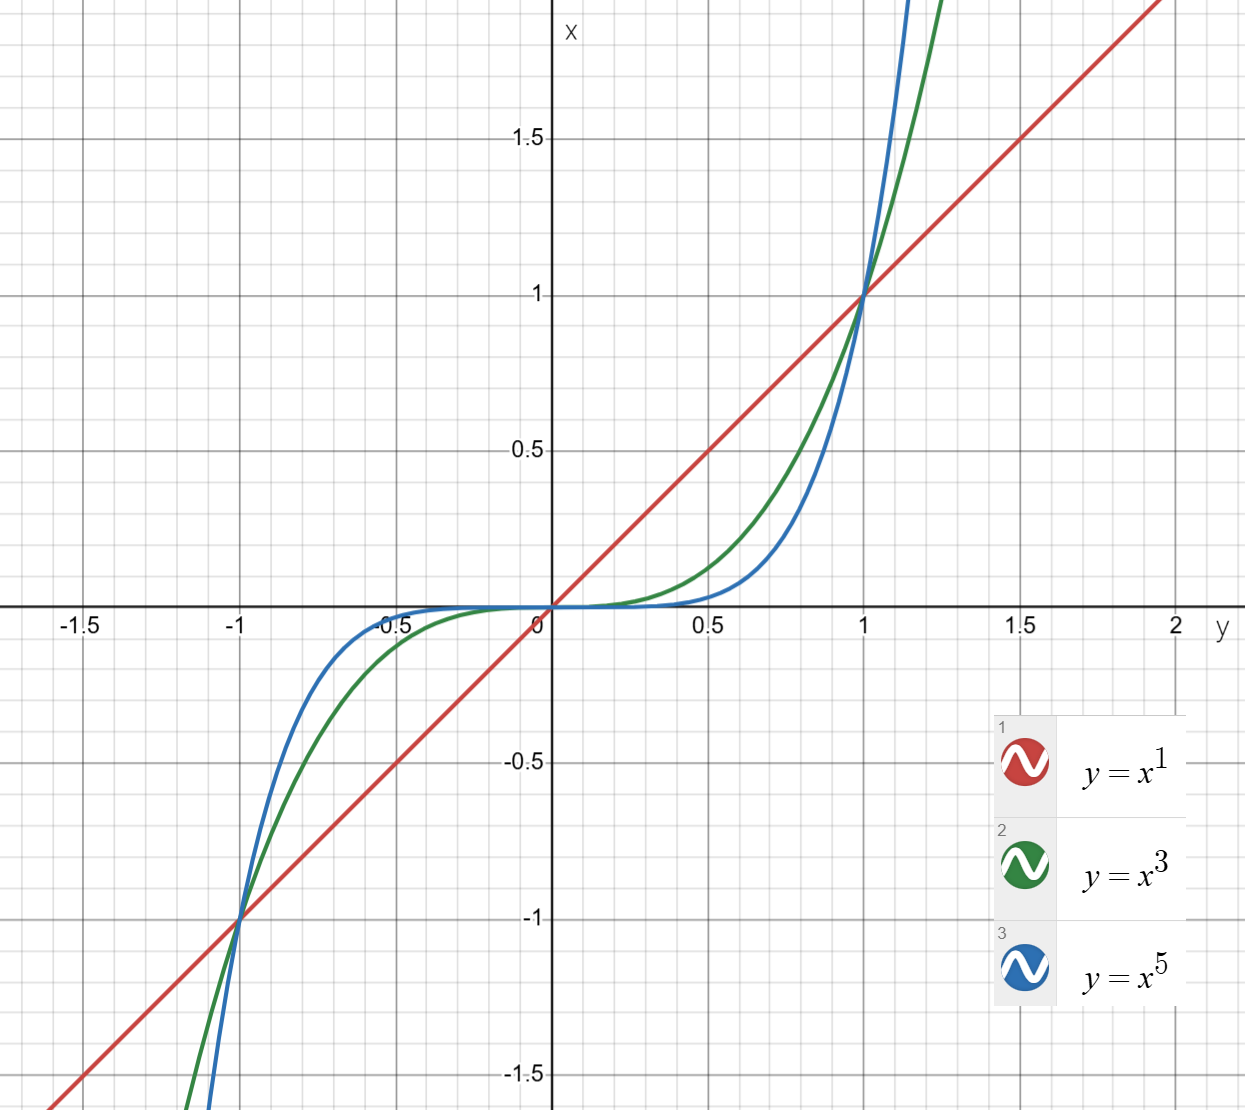
\includegraphics[width=0.5\linewidth]{img/2_liche_fkce.png}
        \caption{grafy funkcí s lichými mocninami}
        \label{fig:enter-label}
    \end{figure}

\subsection{Lineární lomená funkce}
lineární lomená funkce je každá funkce daná předpisem 

$$
f: y=\frac{ax + b}{cx+d}
$$
kde: \\ $a,b,c,d \in \mathbb{R} \\ c \neq 0 \\ ad \neq bc$
Tato funkce je vždy prostá na celém $D(f)$. Grafem je hyperbola s středem v bodě $[-\frac{d}{c}; \frac{a}{c}]$.
\begin{figure}[H]
        \centering
        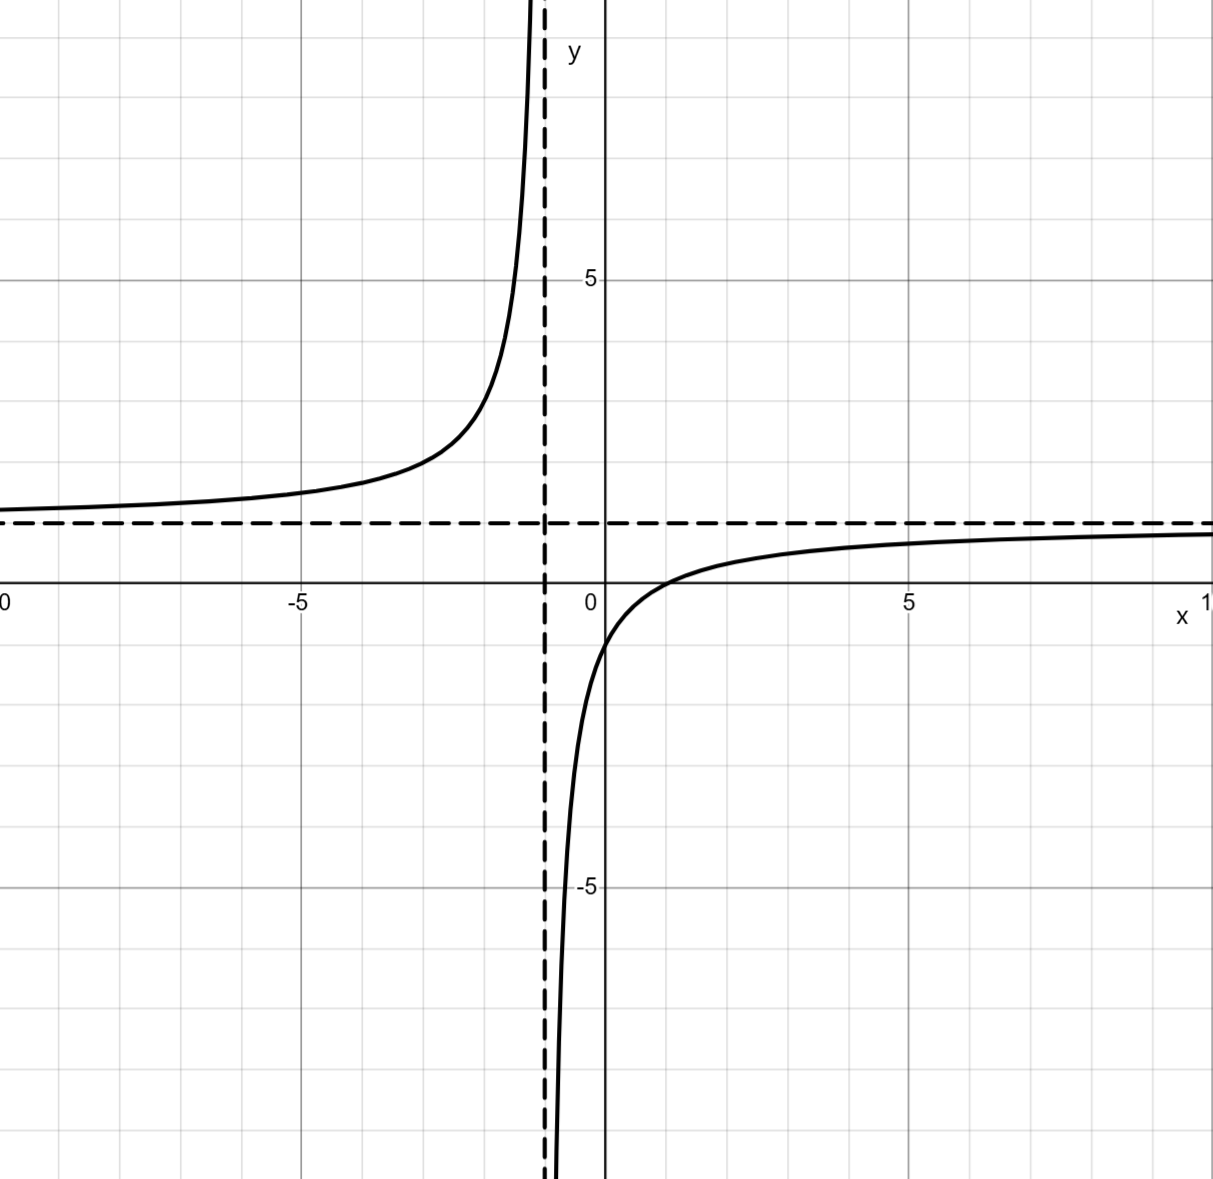
\includegraphics[width=0.5\linewidth]{img/2_lomena_fkce.png}
        \caption{$f(x):$ $y=\frac{x-1}{x+1}$} (čerchovaně jsou asymptoty)
        \label{fig:enter-label}
    \end{figure}

tato konkrétní funkce je v intervalu $\mathbb{R}-\{1\}$, jelikož v $x = -1$ není definována 
\subsubsection{Asymptoty}
Asymptota je taková přímka, jejíž vzdálenost od křivky se limitně blíží k nule, když se jedna nebo obě souřadnice blíží nekonečnu. \\ \\
Co to znamená? funkce se blíží k dané asymptotě do nekonečna, nikdy ji neprotne.\\ \\
Příklad: Určete asymptoty $y=\frac{2x-3}{x-1}$\\
Budou 2 asymptoty. \\
1. získáme určením podmínky $x \neq 1$ první asymptota má rovnici: $x=1$ \\
2. získáme podílem $(2x-3):(x-1)=2\cdot(-\frac{1}{x-1})$. Druhá asymptota má tedy hodnotu $y=2$
graf funkce je:
\begin{figure}[H]
        \centering
        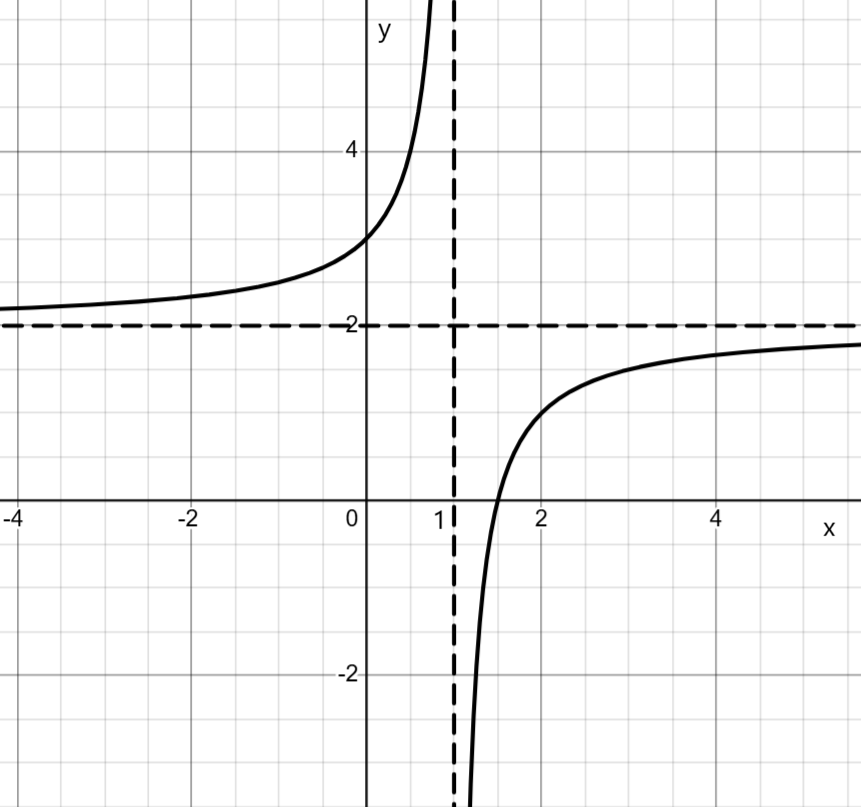
\includegraphics[width=0.5\linewidth]{img/2_lomena_fkce2.0.png}
        \caption{$f(x):$ $y=\frac{2x-3}{x-1}$} (čerchovaně jsou asymptoty)
        \label{fig:enter-label}
    \end{figure}
    

\subsection{Základní vlastnosti funkcí}
\subsubsection{Definiční obor}
Množina $A$ označujeme $D(f)$ a platí pro ni, že $x \in A$
\subsubsection{Obor hodnot}
Obor hodnot je množinou prvků $y \in B$ z nichž ke každému existuje alespoň jeden takový prvek $x\in A$, že $[x,y] \in f$ nazíváme oborem hodnot funkce $f$ a označujeme $H(f)$
\subsubsection{Intervaly monotónnosti}
Intervaly (souvislá množina hodnot), ve kterých je funkce rostoucí nebo klesající
\subsubsection{Sudost Lichost}
Funkce je sudá (souměrná podle osy $y$), pokud splňuje: když do funkce vložíte prvek $x$ a poté inverzní prvek $-x$, pak musí funkce vrátit stejnou výslednou hodnotu. Typickou sudou funkcí je funkce $f: y=x^2$ \\

Funkce se nazývá lichá (je souměrná podle počátku $[0;0]$), pokud splňuje:  \\
1) Pro každé $x \in D(f)$ je také $-x \in D(f)$ \\
2) Pro každé $x \in D(f)$ je $f(-x) = - f(x)$
například funkce: $y=x^3$
\subsubsection{Prostá funkce}
Prostá funkce je v funkcí, která žádnou funkční hodnotu nenabývá vícekrát
\subsection{Grafy vybraných funkcí a jejich vlastnosti}
\subsubsection{Funkce absolutní hodnoty}
\begin{figure}[H]
        \centering
        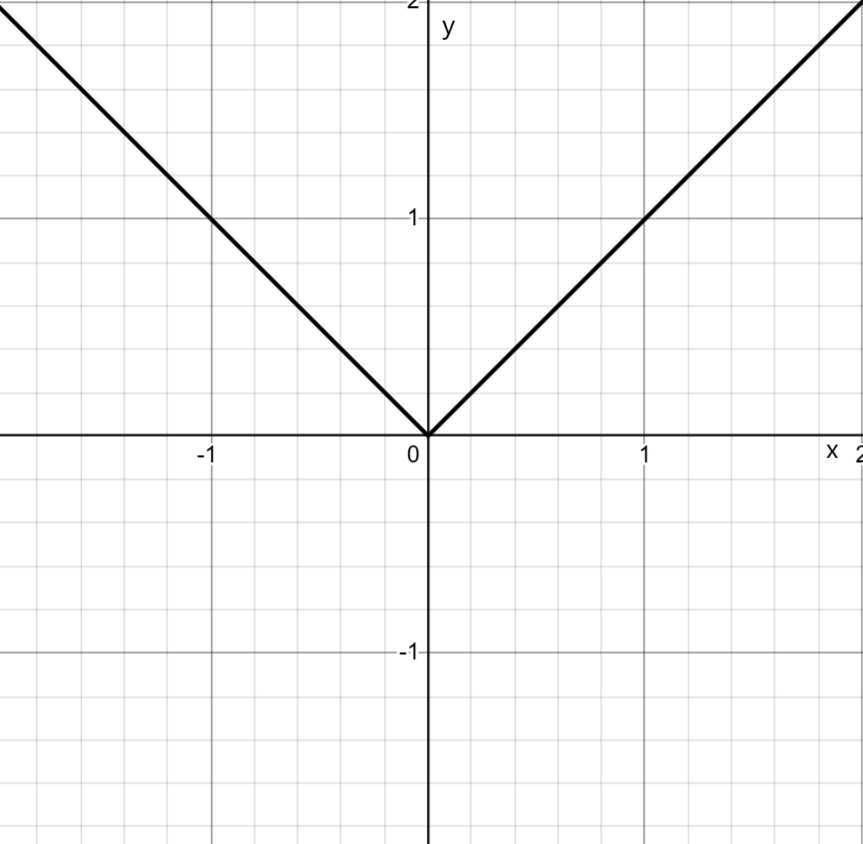
\includegraphics[width=0.5\linewidth]{img/2_absolutni_hodnota.png}
        \caption{$f(x):$ $y=|x|$} 
        \label{fig:enter-label}
    \end{figure}
V intervalu $(-\infty; 0> $ je funkce klesající. V intervalu $<0;\infty)$ je rostoucí. funkce je zdola omezená (má minimum v bodě $[0;0]$). Je sudá.
$$
    D(f)\in \mathbb{R} 
$$
$$
    H(f)\in\langle0;\infty)
$$
\subsubsection{Logaritmická funkce}
\begin{figure}[H]
        \centering
        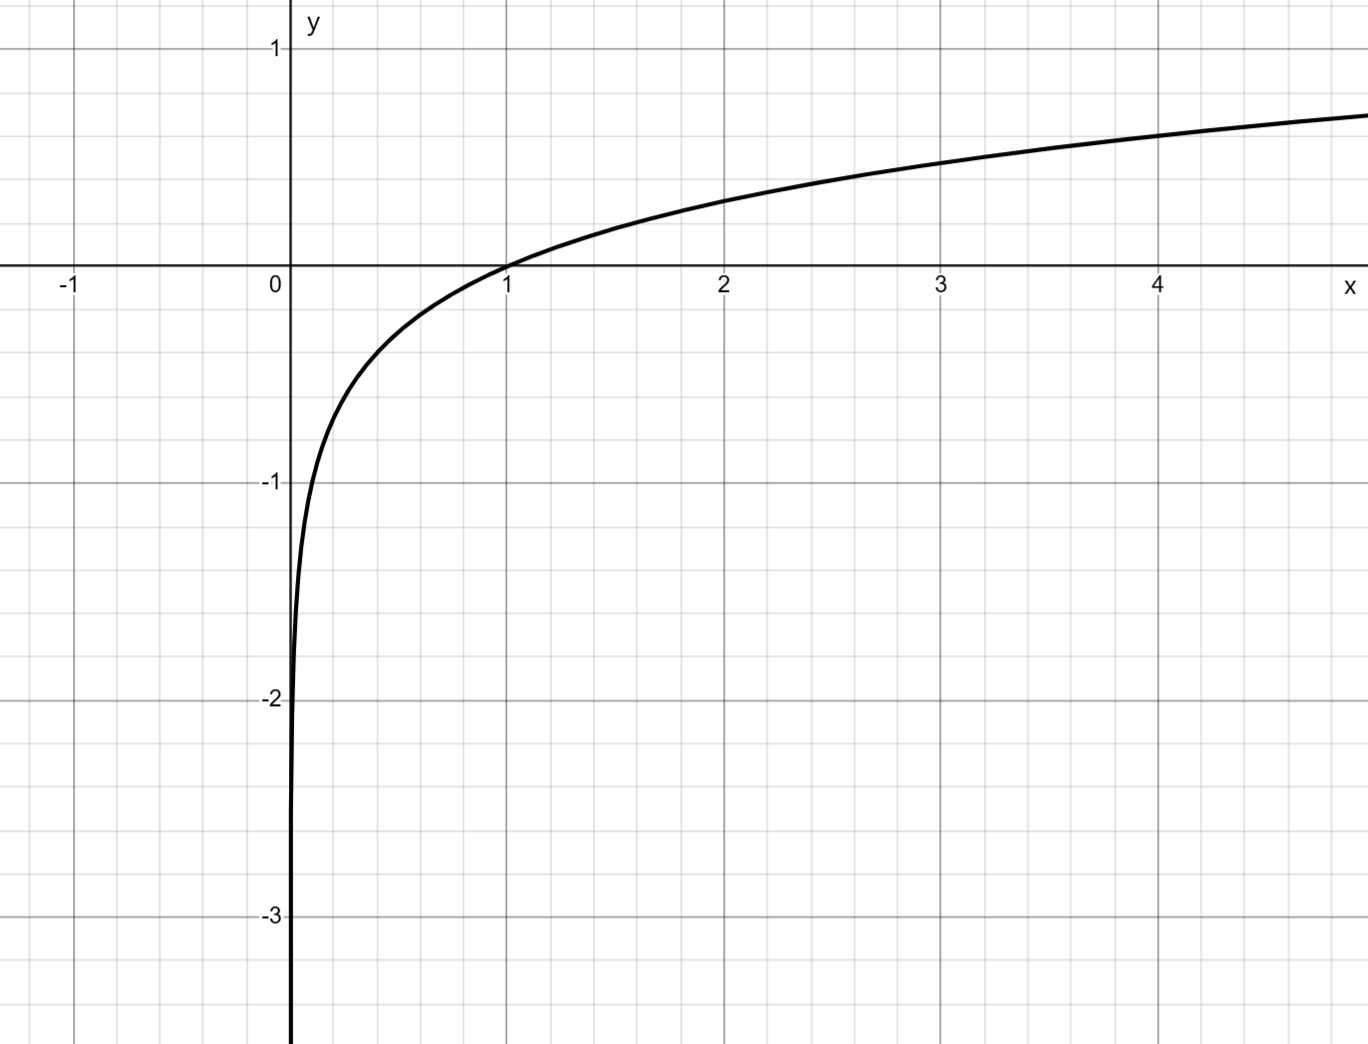
\includegraphics[width=0.5\linewidth]{img/2_logaritmus.png}
        \caption{$f(x): y=log_{10}x$} 
        \label{fig:enter-label}
    \end{figure}
funkce je v celém jejím intervalu $(0;\infty)$ rostoucí. Není omezená. Má lymitu $x=0$
$$
    D(f)\in  (0;\infty)
$$
$$
    H(f)\in\mathbb{R}
$$
\subsubsection{Graf funkce druhé odmocniny}
\begin{figure}[H]
        \centering
        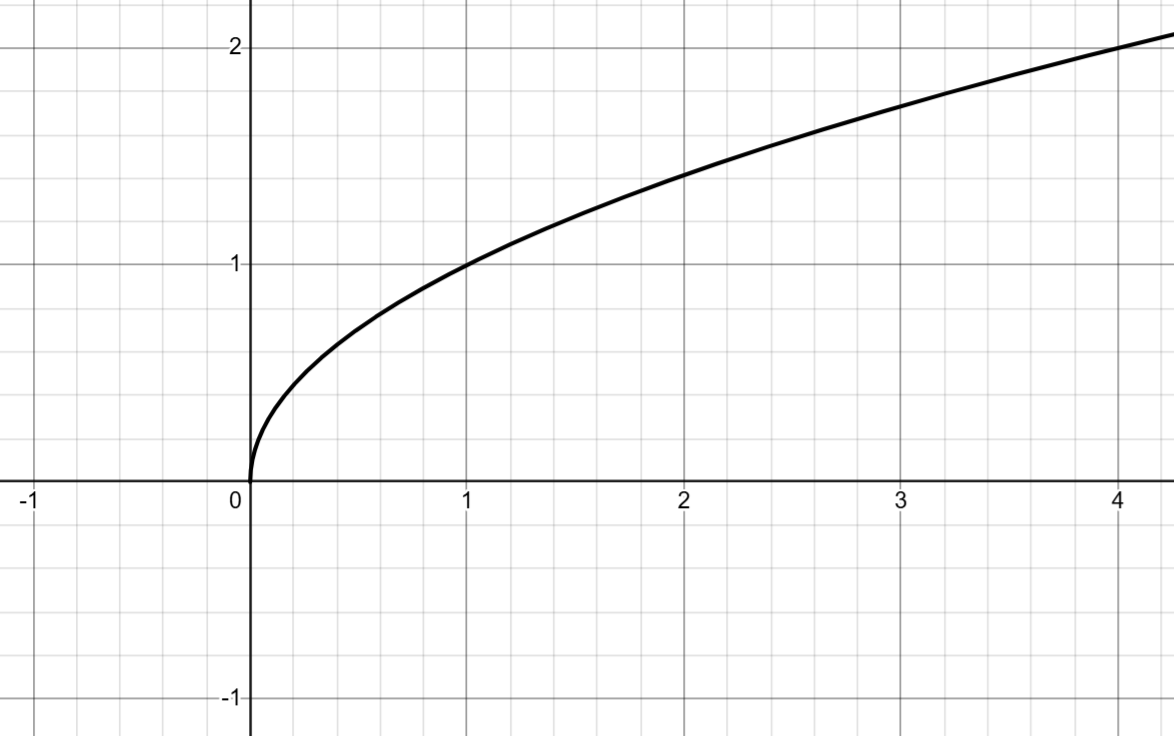
\includegraphics[width=0.5\linewidth]{img/2_odmocnina(x).png}
        \caption{$f(x): y=\sqrt{x}$} 
        \label{fig:enter-label}
    \end{figure}
funkce je v celém jejím intervalu $(0;\infty)$ rostoucí. Je zdola omezená v bodě $[0;0]$
$$
    D(f)\in \langle0;\infty)
$$
$$
    H(f)\in\langle0;\infty)
$$
\subsubsection{Graf funkce třetí odmocniny}
\begin{figure}[H]
        \centering
        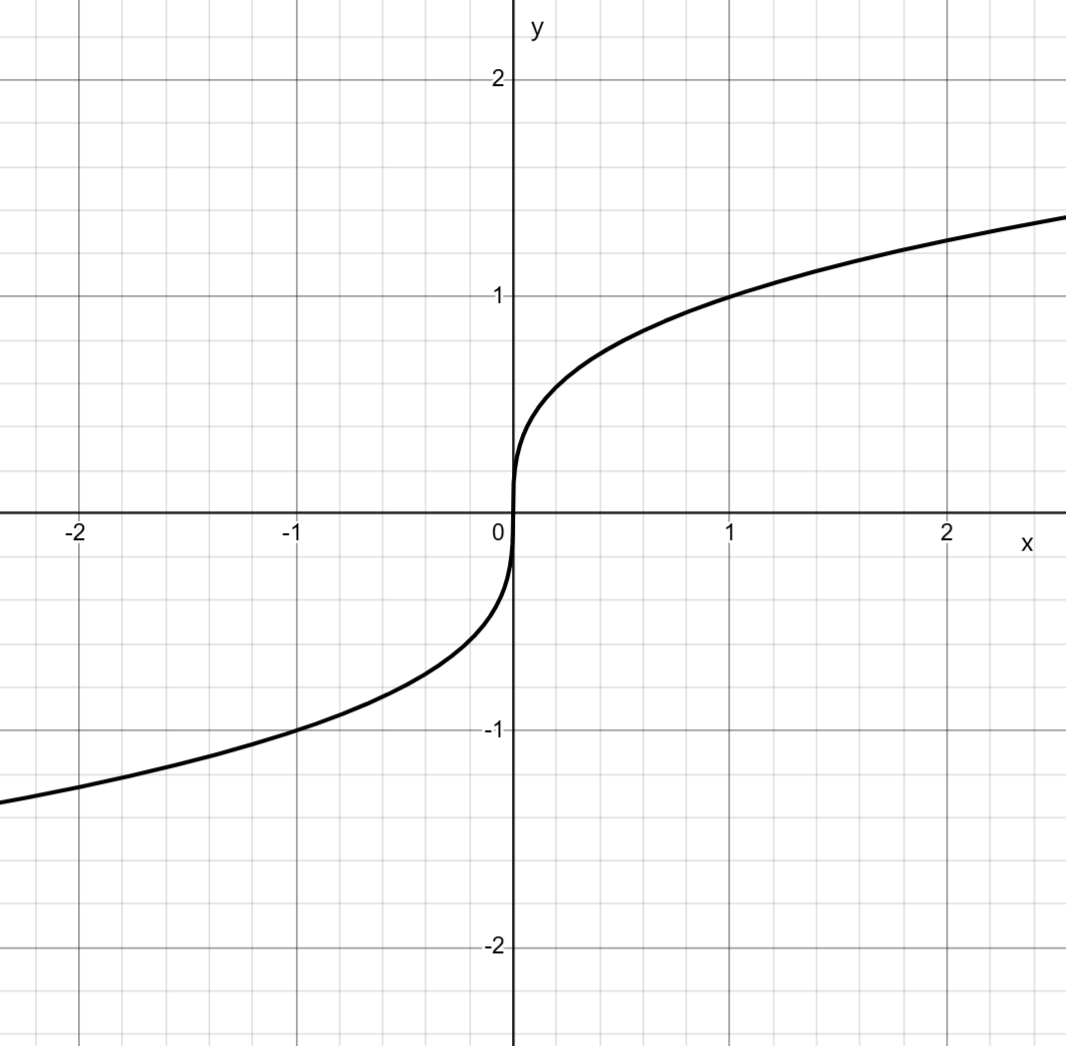
\includegraphics[width=0.5\linewidth]{img/2_3odmocnina(x).png}
        \caption{$f(x): y=\sqrt[3]{x}$} 
        \label{fig:enter-label}
    \end{figure}
funkce je rostoucí
$$
    D(f)\in \mathbb{R} 
$$
$$
    H(f)\in \mathbb{R}
$$




\title{3. Rovnice s parametrem}
\author{Matyáš Horejsek}
\date{26.4.2025}

\maketitle



\section{Rovnice s parametrem}
    \subsection{Obecné rovnice s parametrem}
Rovnice s parametrem jsou rovnice, které obsahují kromě neznámé $x$ ještě další proměnné (označujeme je například $p$), kterým se říká parametry.\\\\
Rovnice s parametrem představují souhrnný zápis množiny rovnic, které bychom získali po dosazení jednotlivých přípustných hodnot za parametry. Řešíme-li rovnice s parametrem, hledáme kořeny v závislosti na hodnotě parametru.\\\\
Parametry ovlivňují hodnotu proměnné s ohledem na provádění operace, a proto musíme provést tzv. diskusi řešení vzhledem k parametru.
    \subsection{Lineární rovnice s parametrem}
Lineární rovnice s parametrem jsou takové rovnice s parametrem, ve kterých se proměnná $x$ vyskytuje pouze v první mocnině.
        \subsubsection{Postup řešení lineární rovnice s parametrem}
\begin{enumerate}
    \item Upravení rovnice a vyjádření neznámé
        \begin{itemize}
            \item Všechny členy s neznámou převedeme na jednu stranu, ostatní na druhou.
            \item Vytkneme neznámou a rovnici upravíme do tvaru:\\
            $$
            k(a)\cdot x=q(a)
            $$
            Kde $x$ je neznámá\\
            $a$ je parametr\\
            a $k(a)$, $q(a)$ jsou výrazy závislé na parametru.
        \end{itemize}
    \item Podmínky pro dělení
        \begin{itemize}
             \item 
               \textbf{Vzorová rovnice:} $(a-2)\cdot x=a+1$\\
            \item
            Pokud chceme rovnici vydělit výrazem s parametrem (například $a-2$), musíme zjistit, kdy je tento výraz roven nule.
            \item \textbf{Nulou dělit nelze!} 
            Proto je nutné rozlišit následující případy:
        \end{itemize}   
                \begin{enumerate}
                        \item Pokud $k(a)\not=0$, tedy $a-2\not=0$, lze dělit a získáváme jedno řešení:
                        $$
                         x=\frac{q(a)}{k(a)}
                        $$
                        Tedy z příkladu:
                        $$
                        x=\frac{a+1}{a-2}
                        $$
                        \item Pokud $k(a)=0$, musíme dosadit tuto hodnotu parametru zpět do původní rovnice a zjistit, zda:
                            \begin{itemize}
                                \item Rovnice je pravdivá pro všechna $x$, tedy má nekonečně mnoho řešení.\\ 
                                $x\in \mathbb{R}$
                                \item Rovnice je nepravdivá pro všechna $x$, tedy nemá řešení.\\
                                $x\not\in \mathbb{R}$
                            \end{itemize}
                \end{enumerate}
    \item Shrnutí výsledků
        \begin{itemize}
            \item Výsledky se často přehledně uvádějí v tabulce tzv. \textbf{Tabulka diskuse}, kde jsou jednotlivé případy podle hodnoty parametru a odpovídající množina řešení.
        \end{itemize}
\end{enumerate}
   
        \textbf{Vzorová tabulka z příkladu:}
        
            \begin{center}
            \begin{tabular}{||c| c||} 
             \hline
             \textbf{Hodnota parametru $a$} & \textbf{Hodnota kořene $K$} \\ [0.5ex] 
             \hline\hline
             $a\not=2$ & $K=\{\frac{a+1}{a-2}\}$ \\
             \hline
             $a=2$ & $K=\emptyset$ \\
             \hline
            \end{tabular}
            \end{center}
  
        \subsubsection{Diskuse k řešení lineární rovnice}
Diskuse řešení lineární rovnice s parametrem spočívá v rozboru všech možných hodnot parametru a určení, jak se pro tyto hodnoty mění množina řešení rovnice. Klíčové je správně určit podmínky, kdy lze dělit výrazem obsahující parametr, a analyzovat speciální případy, kdy tento výraz zaniká.\\\\
\textbf{Obecné zásady diskuse:}
 \begin{itemize}
     \item Vždy určete podmínky, kdy nelze dělit výrazem s parametrem (například kdy je koeficient u $x$ roven nule).
     \item Pro vyloučené hodnoty parametru ověřte, zda má rovnice nekonečně mnoho, jedno nebo žádné řešení.
     \item  Výsledky vždy shrňte přehledně (tabulkou nebo v bodech), kde je jasně vidět závislost řešení na hodnotě parametru.
 \end{itemize}
    \subsection{Kvadratické rovnice s parametrem}
Kvadratické rovnice s parametrem jsou takové rovnice s parametrem, ve kterých se neznámá vyskytuje nejvýše ve druhé mocnině. Je důležité, aby ve druhé mocnině se nacházela neznámá, jinak se nejedná o kvadratickou rovnici. Parametr smí, ale nemusí se nacházet v libovolné $n$-té mocnině.\\
Tedy z obecné rovnice $(a)x^2+(b)x+(c)=0$, kde alespoň jeden koeficient ($a,b,c$) závisí na hodnotě parametru (např. $m$)\\
\textbf{Příklad:}$(m-1)x^2+2mx+(m+2)=0$\\
Než začneme řešit rovnici musíme určit typ rovnice a v jakém případě nám zůstává kvadratickou. Pokud:
\begin{itemize}
    \item $a\not=0$ Rovnice má standardní kvadratický tvar.\\
    Příklad: $(m-1)\not=0$, tedy pro $m\in\mathbb{R}-(1)$
    \item $a=0$ Rovnice se redukuje na lineární $bx+c=0$\\
    Příklad: $(m-1)=0$, tedy $(m-1)x^2...$ nám vypadává.
    \item $a=0$ a současně i $b=0$ rovnice nemá řešení a ztrácí smysl.
\end{itemize}

Při řešení kvadratických rovnic s parametrem musíme provést diskusi řešení vzhledem k parametru, stejně jako u lineárních rovnic s parametrem.
        \subsubsection{Diskuse k řešení kvadratické rovnice s parametrem}
Diskusi provádíme nejprve určením, kdy nám rovnice zůstává kvadratickou a kdy se redukuje na lineární tvar. Poté provedeme \textbf{analýzu diskriminantu}, poté můžeme vše zapsat opět přehledně do tabulky, stejně jako u lineární rovnice. \textbf{POZOR!} Do tabulky uvádíme i případ, kdy se nám kvadratická rovnice redukuje na lineární rovnici.\\\\
Diskriminant $D=b^2-4a\cdot c$, kde je tedy alespoň jeden koeficient ($a, b, c$) závislí na hodnotě parametru, nám určuje počet reálných kořenů:\\
\begin{itemize}
    \item $D>0$: Rovnice má dva reálné kořeny. Graficky má rovnice s osou $x$ dva průsečíky.
    \item $D=0$: Rovnice má jeden reálný kořen. Graficky má rovnice s osou $x$ jeden průsečík a stává se tečnou.
    \item $D<0$: Rovnice nemá žádné reálné kořeny, má pouze komplexně sdružené kořeny. Graficky nemá rovnice s osou $x$ žádný průsečík.
\end{itemize}
\textbf{Vzorová tabulka z příkladu:}
        
            \begin{center}
            \begin{tabular}{||c| c||} 
             \hline
             \textbf{Hodnota parametru $m$} & \textbf{Hodnota kořenů $K$} \\ [0.5ex] 
             \hline\hline
             $m=1$ & $K=\{-\frac{3}{2}\}$ \\
             \hline
             $m<2-\{1\}$ & $K=\{-\frac{1-\sqrt{3}}{2};-\frac{1+\sqrt{3}}{2}\}$ \\
             \hline
             $m=2$ & $K=\{-2\}$\\
             \hline
             $m>2$ & $K=\emptyset$\\
             \hline
            \end{tabular}
            \end{center}

    \subsection{Vztahy mezi kořeny a koeficienty kvadratické rovnice}
Pro kořeny $x_1$, $x_2$ obecné kvadratické rovnice $ax^2+bx+c=0$, případně normované kvadratické rovnice $x^2+\frac{b}{a}x+\frac{c}{a}=0$ kde $a\not=0$ a $a,b,c \in \mathbb{C}$ platí vztahy, které se nazývají Vietovy vzorce.
        \subsubsection{Vietovy vzorce}
Tyto vzorce (vztahy) nám umožňují:
\begin{itemize}
    \item Rychle určit součet a součin kořenů bez jejich explicitního výpočtu.
    \item Sestavit kvadratickou rovnici, známe-li její kořeny.
    \item Rozkládat kvadratické trojčleny na součin dvou lineárních výrazů.
\end{itemize}
\textbf{Vždy musí platit společně:}\\
\begin{center}
            \begin{tabular}{||c| c||} 
             \hline
             $a(x_1+x_2)=-b$ & $a\cdot x_1\cdot x_2=c$ \\
             \hline
             $x_1+x_2=-\frac{b}{a}$ & $ x_1 \cdot x_2=\frac{c}{a}$ \\
             \hline
            \end{tabular}
            \end{center}
\title{4. Soustavy rovnic o více neznámých}
\author{Matyáš Horejsek}
\date{29.4.2025}

\maketitle



\section{Soustavy rovnic o více neznámých}
    \subsection{Obecné poznatky o soustavě rovnic o více neznámých}
Soustavy rovnic o více neznámých jsou matematické úlohy, kde hledáme hodnoty proměnných splňující všechny rovnice současně. Tedy řešením soustavy rovnic o $n$ neznámých se rozumí každá uspořádaná $n$-tice, která splňuje zároveň všechny rovnice soustavy (po dosazení každé rovnice dostaneme pravdivý výrok).\\\\
Mezi nejčastější typy patří rovnice o dvou, třech až čtyřech neznámých. Ty následně dělíme na:
\begin{itemize}
    \item Lineární
    \item Algebraické rovnice vyšších řádů (kvadratické a výše)
    \item Goniometrické
\end{itemize}
Obecný zápis soustavy rovnic o dvou neznámých, kde $a, b, c, d, e, f$ jsou daná reálná čísla a $x, y $ neznámé:\\
$$
ax+by=c
$$
$$
dx+ey=f
$$
Řešením soustavy rovnic o $n$ neznámých nazýváme takovou uspořádanou $n$-tici (dvojicí, trojici,...) a \textbf{výsledek zapisujeme}:
$$
K=\{[x,y,z,...n]\}
$$
    \subsection{Metody řešení soustavy rovnic}
Soustavy rovnic můžeme řešit několika \textbf{početními metodami} a u rovnic se dvěma neznámýma, případně třemi neznámými, můžeme řešit i \textbf{graficky}. Pro dvě neznámé se graficky pohybujeme ve 2D prostoru a pro tři neznámé ve 3D prostoru. 
        \subsubsection{Početní řešení soustavy rovnic}
Soustavy rovnic můžeme řešit dvěma základními metodami, které se dají uplatnit u všech rovnic o $n$ neznámých:\\
\textbf{Vzorový příklad rovnice o dvou neznámých:}
$$
3x+y=7
$$
$$
x-2y=-4
$$
\begin{itemize}
    \item \textbf{Dosazovací metoda}
        \begin{enumerate}
            \item Vyjádříme jednu proměnnou z jedné rovnice, například: 
                $$
                x=2y-4
                $$
            \item Dosadíme do druhé rovnice a vyřešíme:
                $$
                3(2y-4)+y=7
                $$
                $$
                y=\frac{19}{7}
                $$
            \item Získanou neznámou dosadíme zpět do původní rovnice a vyřešíme ji pro druhou neznámou:
                $$
                3x+\frac{19}{7}=7
                $$
                $$
                x=\frac{10}{7}
                $$
                $$
                K=\{[\frac{10}{7}, \frac{19}{7}]\}
                $$
        Pro ověření můžeme dosadit obě neznámé zpět do původní soustavy rovnic a vypočítat. Vyjadřovat neznámé z rovnice a dosazovat je zpět pro následný výpočet, se pokoušíme vždy co nejrozumněji. 
        \end{enumerate}

    \item \textbf{Eliminační (sčítací) metoda}
        \begin{enumerate}
            \item Úpravou rovnic a následným sečtením, nebo odečtením, odstraníme jednu neznámou:
                $$
                3x+y=7 /\cdot2
                $$
                $$
                x-2y=-4
                $$
                Upravíme si první rovnici a rovnice mezi sebou sečteme:
                $$
                6x+2y+x-2y=14-4
                $$
            \item Vznikne jednoduchá rovnice s jednou neznámou, kterou vyřešíme:
                $$
                7x=10
                $$
                $$
                x=\frac{10}{7}
                $$
            \item Vyřešenou neznámou dosadíme zpět do původní rovnice a vyřešíme druhou neznámou:
                $$
                \frac{10}{7}-2y=-4
                $$
                $$
                y=\frac{19}{7}
                $$
                $$
                K=\{[\frac{10}{7}, \frac{19}{7}]\}
                $$
        \end{enumerate} 
        
    \item \textbf{Substituční metoda}\\
        Substituční metoda je doplňkový způsob jak řešit soustavy rovnice o více neznámých. Využijeme ji primárně u soustav o třech a více neznámých, ale i u například soustav, kde je neznámá v mocnině. Ne vždy se, ale vyplatí využít substituci, proto nepatří mezi základní metody řešení soustav rovnic o více neznámých:\\
        \textbf{Příklad:}
        $$
        \frac{2}{x+y}-\frac{5}{x-y}=1
        $$
        $$
        \frac{1}{x+y}+\frac{4}{x-y}=\frac{9}{5}
        $$
        \begin{enumerate}
            \item Nejprve si určíme co nahradíme substitucí za jinou neznámou, případně neznámé:
                $$
                a=\frac{1}{x+y}    
                $$
                $$
                b=\frac{1}{x-y}
                $$
            \item Nově vzniklé neznámé dosadíme zpět do původní soustavy rovnic:
                $$
                2a-5b=1
                $$
                $$
                a+4b=\frac{9}{5}
                $$
            \item Nově vzniklou snazší soustavu rovnic vyřešíme s pomocí dosazovacích a sčítacích metod a najdeme výsledky pro nové neznámé:
                $$
                2a-5b=1
                $$
                $$
                a+4b=\frac{9}{5}/\cdot(-2)
                $$
                Rovnice sečteme a dořešíme. Výsledek opět vrátíme do upravených rovnic a vyřešíme pro druhou neznámou:
                $$
                b=\frac{1}{5}
                $$
                $$
                a=1
                $$
            \item Pokud známe hodnoty neznámých, které jsme si vytvořili, vrátíme tyto hodnoty do substitučních rovnic:
                $$
                1=\frac{1}{x+y}
                $$
                $$
                \frac{1}{5}=\frac{1}{x-y}
                $$
            \item Nově vzniklou snazší soustavu rovnic opět vyřešíme s pomocí dosazovacích a sčítacích metod a zjistíme hodnoty neznámých:
            $$
            x=3
            $$
            $$
            y=-2
            $$
            $$
            K=\{[3,-2]\}
            $$
        \end{enumerate}
\end{itemize}

U soustav rovnic se \textbf{třemi a více} neznámými využíváme i další pokročilejší metody, které se studují hlavně až na vysokých školách (následující informace slouží pro ilustraci a jejich znalost není klíčová):
\begin{itemize}
    \item Gaussova eliminace
    \item Využití matic
\end{itemize}

        \subsubsection{Grafické řešení soustavy rovnic}
Každá rovnice vyjadřuje geometrický objekt:
\begin{itemize}
    \item Rovnice o dvou neznámých se graficky zobrazí jako přímka v rovině.
    \item Rovnice o třech neznámých se graficky zobrazí jako rovina v prostoru.
    \item Lineární rovnice s $n$ proměnnými se graficky zobrazí jako hyperrovina v $n$D prostoru.
\end{itemize}
Řešení soustavy odpovídá společnému bodu všech těchto objektů, tedy jejich průsečíku.
Grafické řešení pomáhá pochopit koncept řešení soustavy jako průniku více podmínek najednou.\\\\
Pokud řešíme soustavu graficky, musíme si soustavy převést do tvaru:
$$
y=ax+b
$$
\textbf{Příklad:}
$$
y=2x+1
$$
$$
y=-x+4
$$
\begin{enumerate}
    \item Nejdříve obě převedené rovnice zaznačíme do souřadnicové roviny ($xy$-roviny)
    \item Následně hledáme bod (body), kde se protínají – to je řešení soustavy.
\end{enumerate}
\begin{figure}[H]
        \centering
        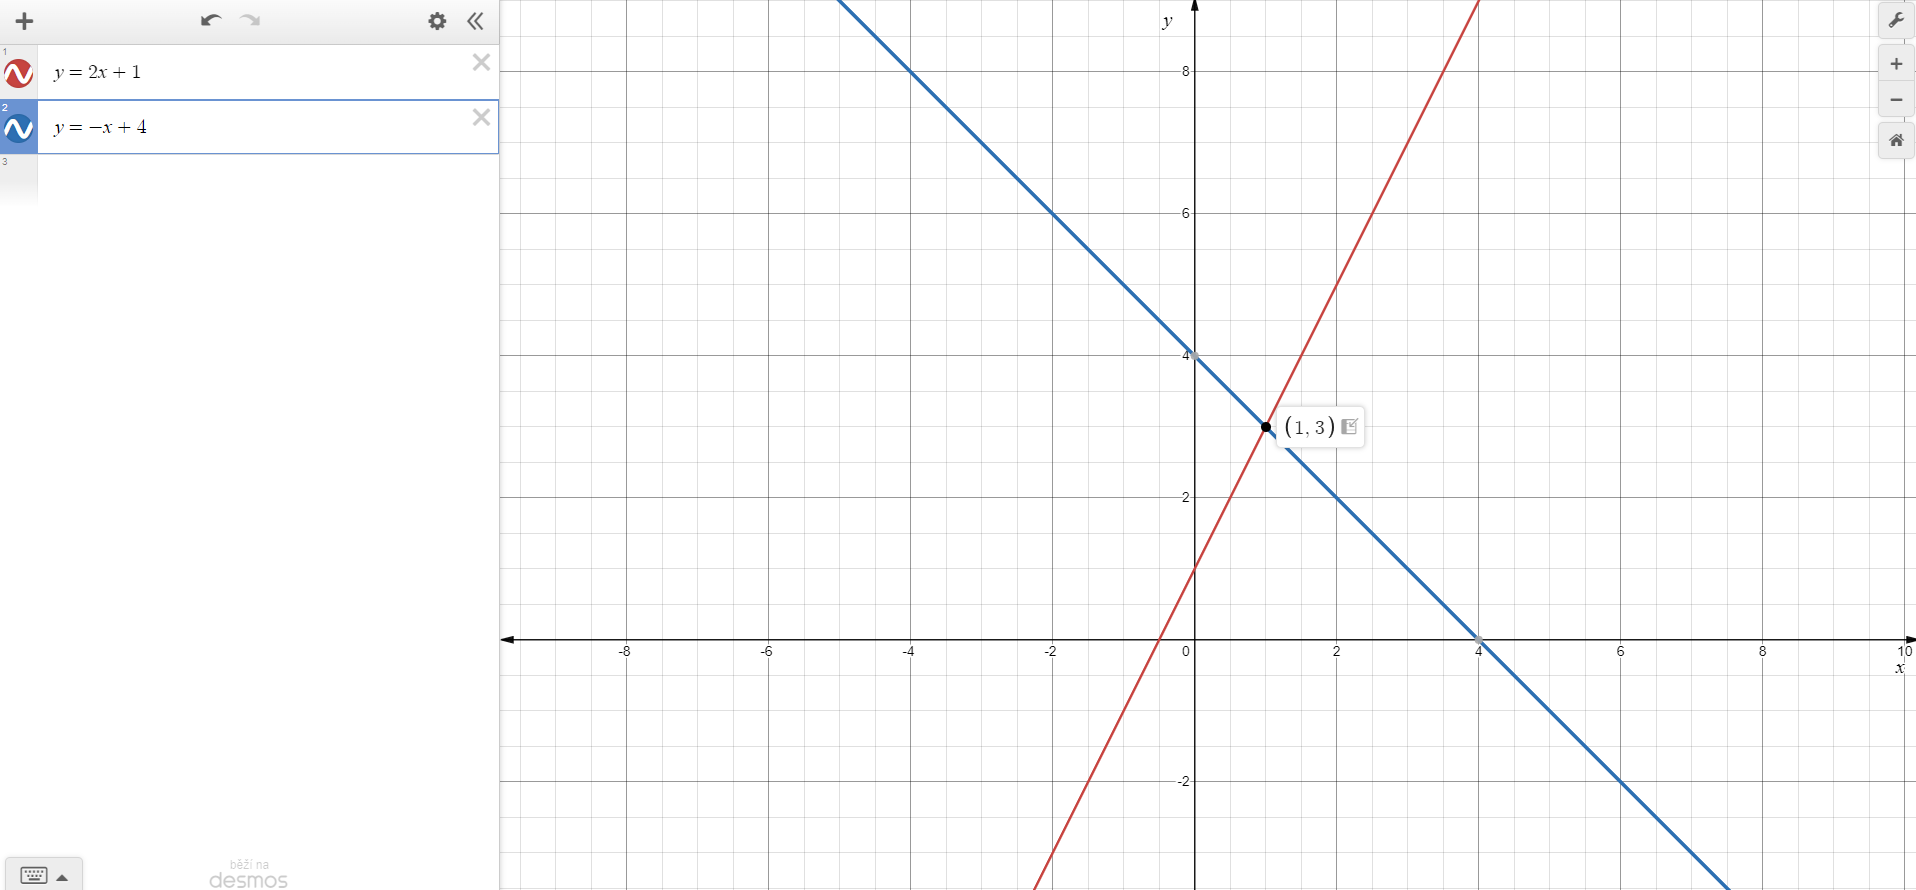
\includegraphics[width=0.5\linewidth]{img/4_soustava linearnich rovnic o dvou neznamych.png}
        \caption{$y=2x+1;y=-x+4$} 
        \label{fig:enter-label}
    \end{figure}
    
    \subsection{Počet řešení soustavy rovnic}
Nejsnazší zjištění počtu řešení je pře grafické řešení.\\
Pokud řešíme soustavu rovnic o \textbf{dvou neznámých} tak počet řešení odpovídá následujícím podmínkám:
 \begin{center}
            \begin{tabular}{||c| c|c||} 
             \hline
             \textbf{Situace} & \textbf{Geometrický význam} & \textbf{Počet řešení} \\ [0.5ex] 
             \hline\hline
             Přímky se protínají & Jediný průsečík & \textbf{Jedno řešení} \\
             \hline
             Přímky se překrývají & Jsou totožné & \textbf{Nekonečně mnoho řešení} \\
             \hline
             Přímky jsou rovnoběžné & Nikdy se neprotínají & \textbf{Žádné řešení}\\
             \hline
            \end{tabular}
            \end{center}
Ukázku můžete vidět v předešlém příkladu.\\\\
Pokud řešíme soustavu rovnic o \textbf{třech neznámých} tak počet řešení odpovídá následujícím podmínkám:
\begin{center}
            \begin{tabular}{||c| c|c||} 
             \hline
             \textbf{Situace} & \textbf{Geometrický význam} & \textbf{Počet řešení} \\ [0.5ex] 
             \hline\hline
             Tři roviny se protínají v jednom bodě & Společný průsečík všech & \textbf{Jedno řešení} \\
             \hline
             Tři roviny se protínají v přímce & Mají společnou přímku & \textbf{Nekonečně mnoho řešení} \\
             \hline
             Rovnoběžné nebo se neprotínají & Žádný společný bod & \textbf{Žádné řešení}\\
             \hline
            \end{tabular}
            \end{center}
\textbf{Příklad} tří rovin, které mají společný průsečík:
\begin{figure}[H]
        \centering
        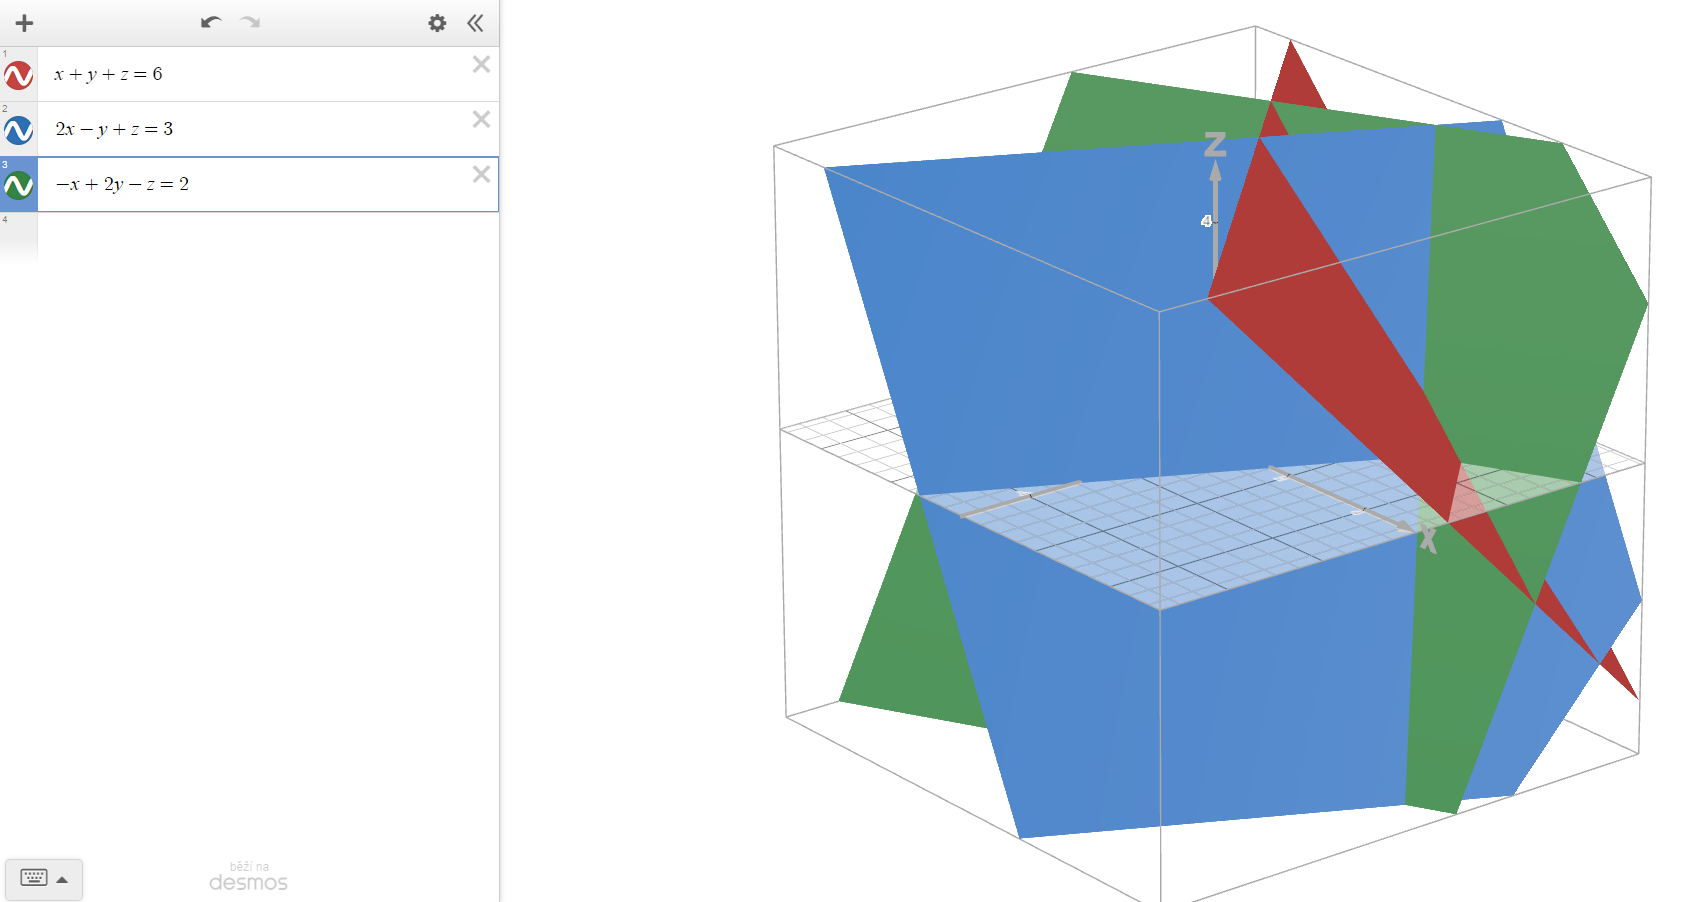
\includegraphics[width=0.5\linewidth]{img/4_soustava_rovnic_o_trech_neznamych.png}
        \caption{$y=6-x-z;y=2x+z-3;y=\frac{2+z+x}{2}$} 
        \label{fig:enter-label}
    \end{figure}
\title{5. Exponenciální a logaritmická funkce}

\author{Jan Peroutka}
\maketitle

\section{Exponenciální a logaritmická funkce}

\subsection{Exponenciální funkce}
Exponenciální funkce je každá funkce tvaru
$$
f(x) = a^x,
$$
kde $a > 0$, $a \ne 1$ a $x \in \mathbb{R}$.

\subsubsection{Vliv základu $a$ na průběh}
\begin{itemize}
    \item Pokud $a > 1$, je funkce rostoucí.
\begin{figure}
            \centering
            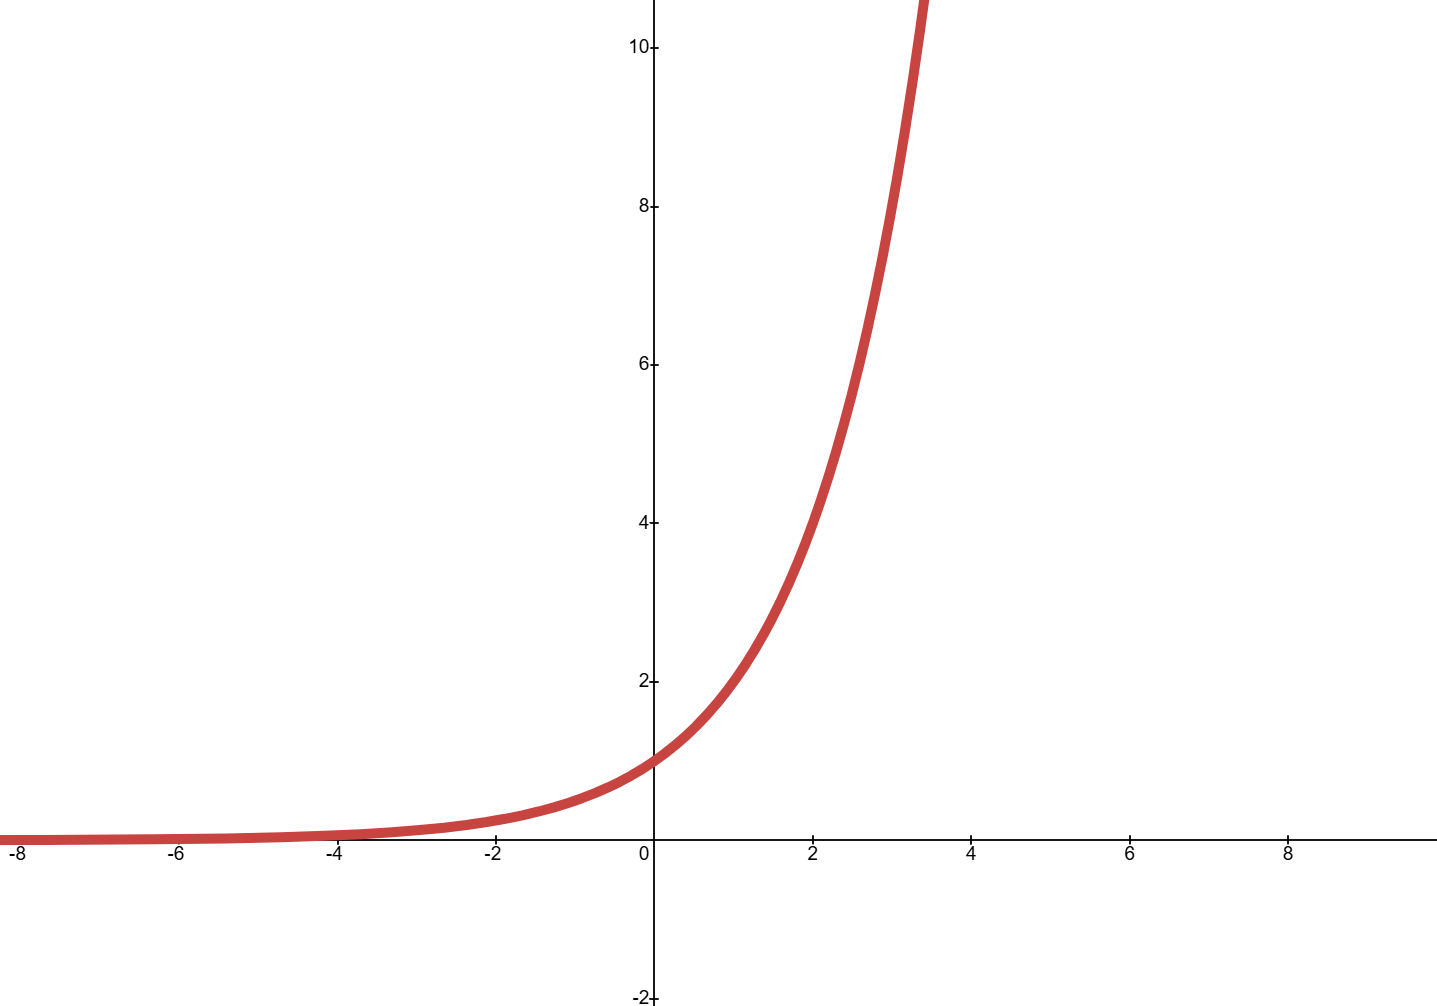
\includegraphics[width=0.5\linewidth]{img/5_exp_ros.png}
            \caption{$y = 2^x$}
        \end{figure}
    \item Pokud $0 < a < 1$, je funkce klesající.
\begin{figure}
    \centering
    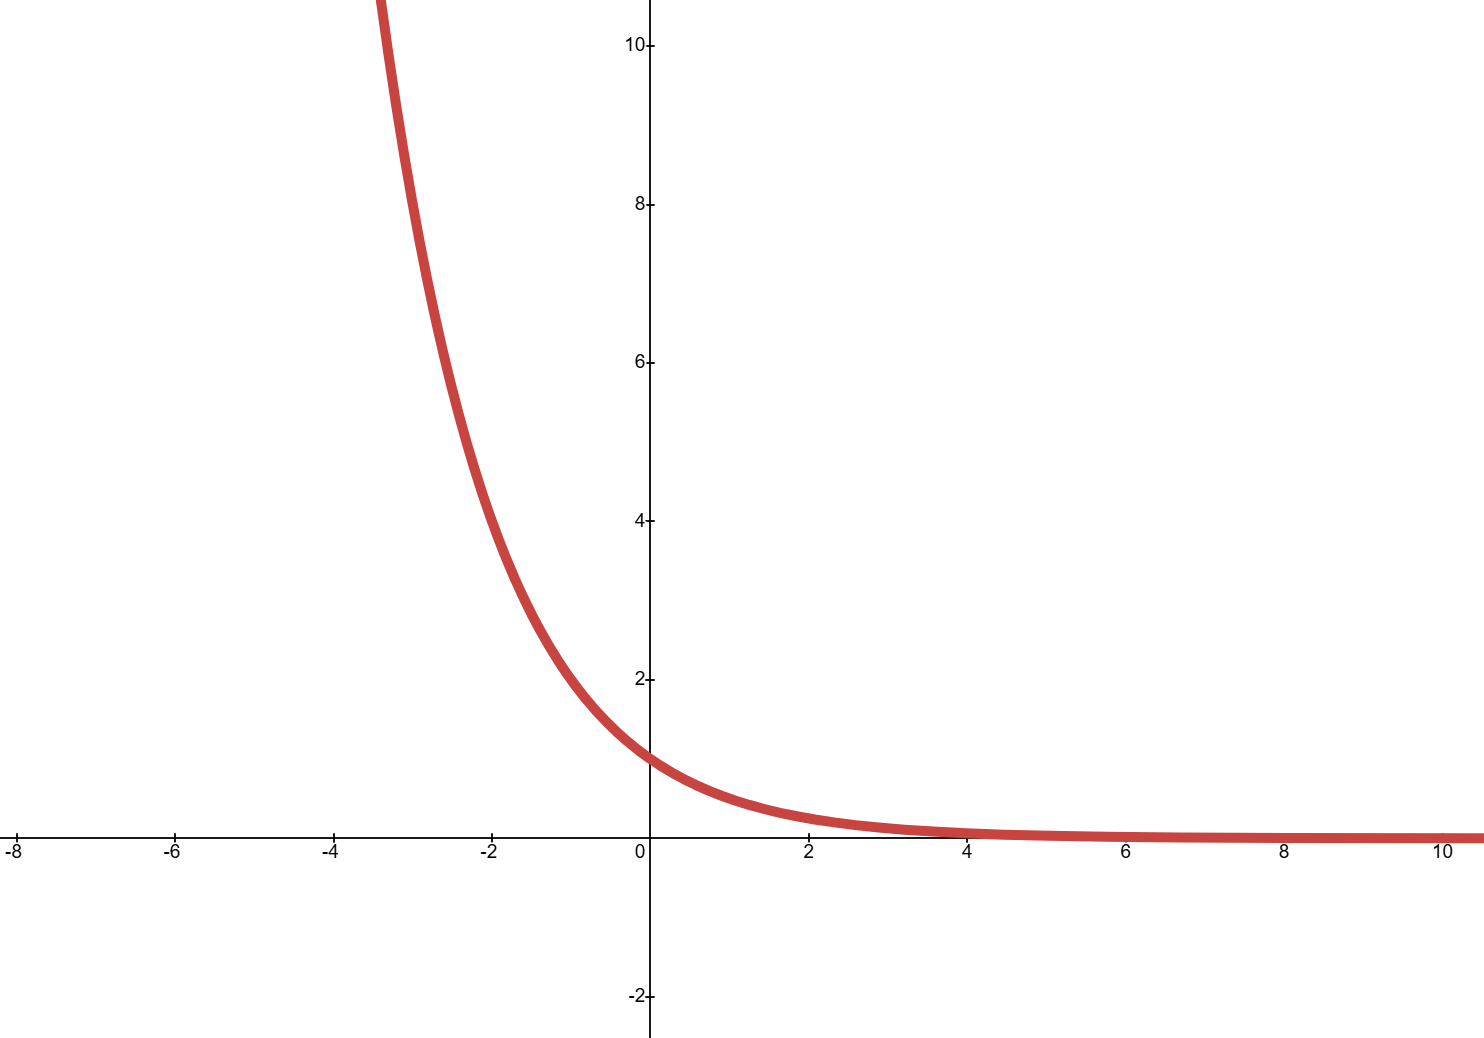
\includegraphics[width=0.5\linewidth]{img/5_exp_kles.png}
    \caption{$y = (\frac{1}{2})^x$}
\end{figure}
\end{itemize}
\textbf{Graf vždy prochází bodem $[0, 1]$.}

\subsubsection{Definiční obor a obor hodnot}
\begin{itemize}
    \item Definiční obor: $D(f) = \mathbb{R}$
    \item Obor hodnot: $H(f) = (0, \infty)$
\end{itemize}

\subsection{Logaritmická funkce}
Logaritmická funkce je inverzní funkcí k exponenciální funkci. Její obecný tvar je:
$$
f(x) = \log_a x,
$$
kde $a > 0$, $a \ne 1$, $x > 0$.

\subsubsection{Vliv základu $a$ na průběh}
\begin{itemize}
    \item Pokud $a > 1$, je funkce rostoucí.
\begin{figure}
        \centering
        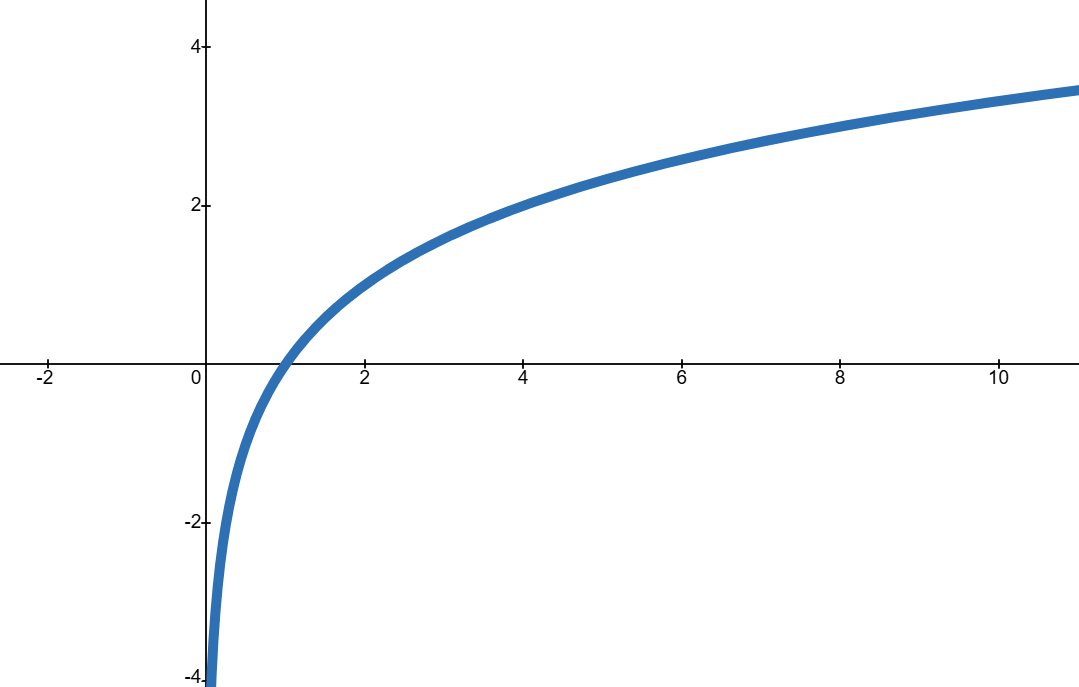
\includegraphics[width=0.5\linewidth]{img/5_log_ros.png}
        \caption{$y=\log_2 x
$}
    \end{figure}
        \item Pokud $0 < a < 1$, je funkce klesající.
\begin{figure}
    \centering
    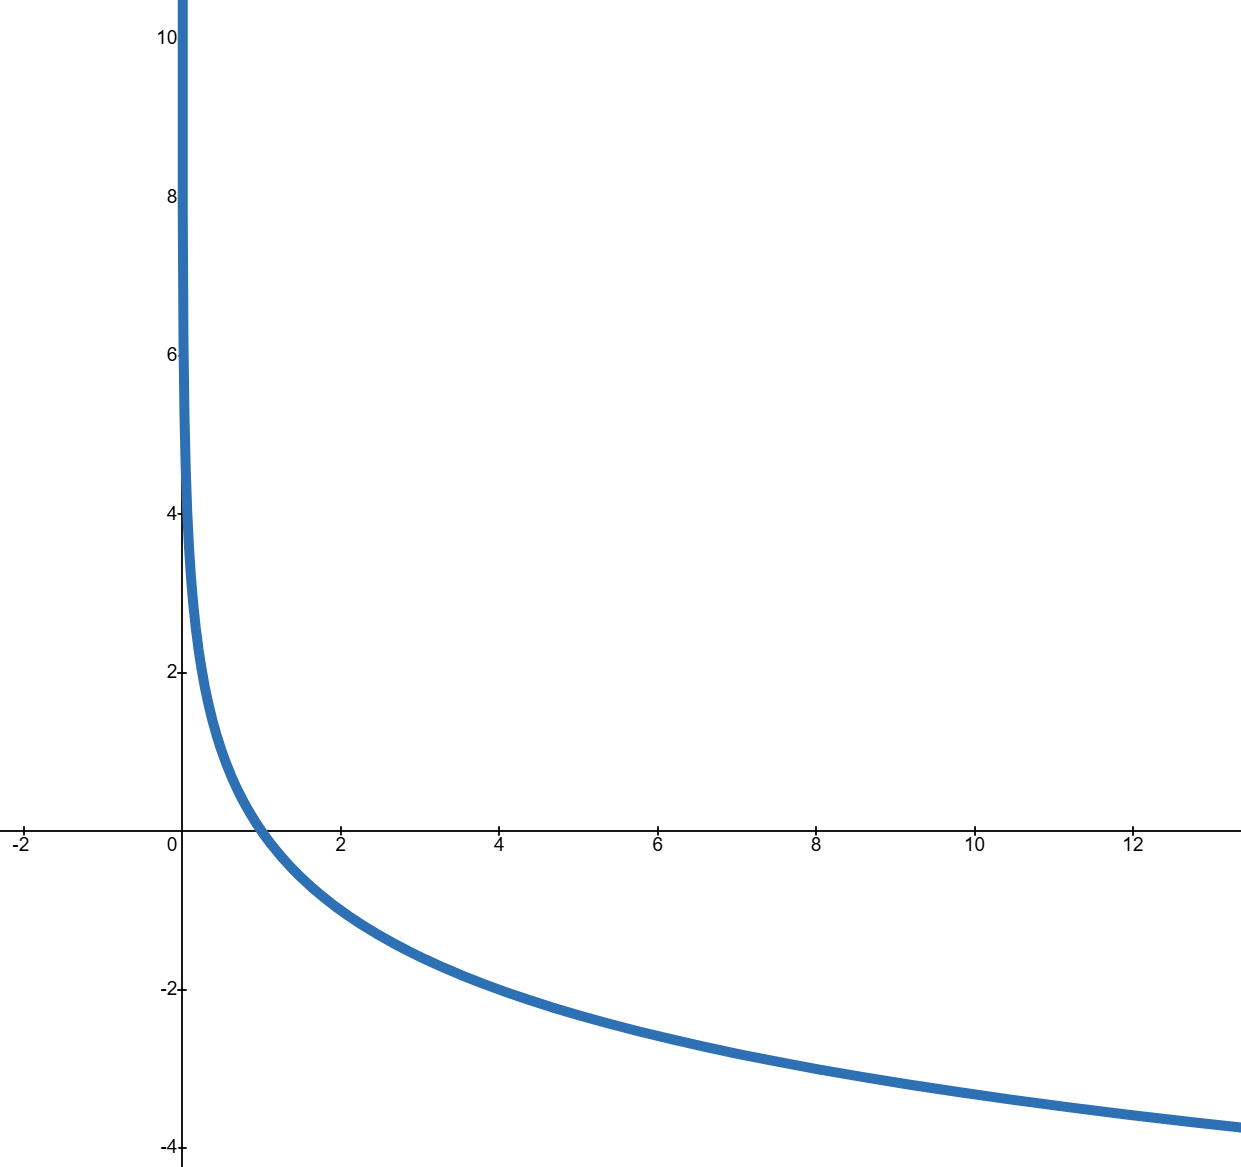
\includegraphics[width=0.5\linewidth]{img/5_log_kles.png}
    \caption{$y=\log_{\frac{1}{2}} x
$}
\end{figure}
\end{itemize}
Graf vždy prochází bodem $[1, 0]$.
\subsubsection{Definiční obor a obor hodnot} 
\begin{itemize}
    \item Definiční obor: $D(f) = (0, \infty)$
    \item Obor hodnot: $H(f) = \mathbb{R}$
\end{itemize} 
\subsection{Vztah mezi exponenciální a logaritmickou funkcí}
Funkce $f(x) = a^x$ a $f^{-1}(x) = \log_a x$ jsou navzájem inverzní. To znamená:
$$
a^{\log_a x} = y \quad \text{a} \quad \log_a(a^x) = y.
$$
Grafy těchto funkcí jsou zrcadlově souměrné podle osy $y = x$.

\subsection{Představa logaritmu}
Logaritmus je odpovědí na otázku: „Na kolikátou musím umocnit číslo $a$, abych dostal číslo $x$?“
$$
\log_a x = y \Leftrightarrow a^y = x.
$$
\subsection{Základní pravidla pro počítání s mocninami a logaritmy}
\subsubsection{Mocniny}
Pro všechna $a > 0$, $m, n \in \mathbb{R}$:
\begin{itemize}
    \item $a^m \cdot a^n = a^{m+n}$
    \item $\frac{a^m}{a^n} = a^{m-n}$
    \item $(a^m)^n = a^{m \cdot n}$
    \item $a^{-n} = \frac{1}{a^n}$
    \item $a^0 = 1$
    \item $\sqrt[n]{a^b} = a^{\frac{b}{n}}$
\end{itemize}

\subsubsection{Logaritmy}
Pro všechna $a, x, y > 0$, $a \ne 1$:
\begin{itemize}
    \item $\log_a(x \cdot y) = \log_a x + \log_a y$
    \item $\log_a\left(\frac{x}{y}\right) = \log_a x - \log_a y$
    \item $\log_a(x^r) = r \cdot \log_a x$
    \item $\log_a a = 1$; $\log_a 1 = 0$
    \item Změna základu: $\log_a x = \frac{\log_b x}{\log_b a}$
\end{itemize}

\title{6 Exponenciální a logaritmické rovnice a nerovnice}
\author{Roman Šnajder}
\date{April 2025}

\maketitle

\section{Exponenciální a logaritmické rovnice a nerovnice}
\subsection {Exponenciální rovnice}

Z běžné rovnice se exponenciální stává, pokud obsahuje proměnnou v exponentu. Typickým příkladem exponenciální rovnice může být třeba $2^x = 8$.
\subsection {Pravidla pro počítání s exponenty}
$$a^x\cdot a^y=a^{x+y}$$
$$a^{-x}=\frac{1}{a^x}$$
$$a^{x^{y}}=a^{xy}$$
$$a^{x-y}=\frac{a^x}{a^y}$$
$$a^0=1$$
Rovnice typu $a^{f(x)}=a^{g(x)}$ se řeší porovnáním exponentů (pro $a>0$, a $\neq 1$). Rovnice typu $a^{f(x)}=b^{g(x)}$, se řeší logaritmováním na tvar $f(x)\cdot\log_a a=g(x)\cdot\log_a b$ (pro $a>0$, $b>0$, $a\neq1$, $b\neq1$)
\subsubsection{Jednoduchá exponenciální rovnice}
Při řešení exponenciální rovnici, je žádoucí, pokud lze rovnici upravit na tvar o stejném základu na obou stranách rovnice.
$$2^3=8$$
$$2^x=2^3$$
$$x=3$$
Další případ nastává, pokud se na jedné straně rovnice vyskytuje jednička. Základ obsahující číslo 1 je možné zapsat jako libovolné číslo na nultou a tím vznikne exponenciální rovnice o stejném základu.
$$5^x=1$$
$$5^x=5^0$$
$$x=0$$
V exponenciální rovnici lze využít i substituce, kdy členy s neznámou jsou nahrazeny písmenem, které však po vypočtení nově vzniklé rovnice musí být dosazeno zpět do původního výrazu a až tento výsledek je řešením dané rovnice. Při použití této metody často vznikne kvadratická rovnice.
$$9^x-25\cdot3^x-54=0$$
$$3^{2x}-25\cdot3^x-54=0$$
$$t^2-25t-54=0$$
$$(t+2)\cdot(t-27)=0$$
$$3^x=-2,x_1\neq R$$
$$3^x=27$$
$$x_2=3$$
\subsection {Exponenciální nerovnice}
Exponenciální nerovnice se řeší stejně jako rovnice. Liší se pouze u výsledku, kdy u nerovnice vznikne interval nebo intervaly. Pokud je neznámá menší než 0, pak se nerovnost vynásobí (-1).
$$2^{1-x}>\frac{1}{2}$$
$$2^{1-x}>2^{-1}$$
$$1-x>-1$$
$$-x>-2 /\cdot(-1)$$
$$x<2$$
$$K=(-\infty;2)$$
Stejně jako u rovnice i zde lze použít substituce s tím rozdílem, že řešením bude interval nebo intervaly, pro které má daná rovnice řešení.
$$9^x-25\cdot3^x-54>0$$
$$3^{2x}-25\cdot3^x-54>0$$
$$t^2-25t-54>0$$
$$(t+2)\cdot(t-27)>0$$
$$\begin{tabular}{c|c|c}
    - & + & + \\
    - & - & + 
\end{tabular}$$
$$x=(-\infty;-2)\cup(27;\infty)$$
\subsection {Pravidla pro počítání s logaritmy}
$$\log_{a}x+\log _{a}y=\log_{a}(xy)$$
$$\log_{a}x-\log_{a}y=\log_{a}\frac{x}{y}$$
$$\log_{a}x^y=y\cdot\log_{a}x$$
$$\log_{a}a=1$$
$$\log_{a}x=\frac{\log_c x}{\log_c a}$$
\subsubsection{Logaritmické rovnice}
Základní logaritmická rovnice s užitím pravidla. Zde však musí být určeny podmínky, jelikož logaritmus nemůže být záporný a tak budu řešit pouze pro x, která nám vyjdou kladná. (V tomto případě čísla $x \in (0;\infty)$)
$$\log_{2}x=3$$
$$x=2^3$$
$$x=8$$
Pokud je v příkladu logaritmus a k tomu nějaké další číslo, pak z tohoto čísla vytvoříme logaritmus a příklad se vyřeší podobně jako ten předchozí. Opět musí být určen definiční obor $$(1;\infty)$$\\
$$\log_{2}(x-1)+2=\log_{2}(2x+1)$$
$$\log_{2}(x-1)+\log_{2}4=\log_{2}(2x+1)$$
$$\log_{2}[(x-1)\cdot4]=\log_{2}(2x+1)$$
$$4x-4=2x+1$$
$$x=\frac{5}{2}$$
U logaritmický nerovnice opět použít substituce.
$$\log_{2}^2x-2log_{2}x+1=0$$
$$\log_{2}x=t$$
$$t^2-2t+1=0$$
$$(t-1)^2=0$$
$$\log_{2}x=1, x=2$$
\subsubsection{Logaritmické nerovnice}
Logaritmické nerovnice se řeší stejně jako rovnice. Liší se pouze u výsledku, kdy u nerovnice vznikne interval nebo intervaly. I u nerovnic lze použít substituce. Pokud je základ logaritmu menší než 1, pak se nerovnost musí otočit! Dalším důležitým krokem je si, tak jako u rovnic, určit definiční obor.
$$\log_{\frac{1}{2}}(2-x)<-3$$
$$\log_{\frac{1}{2}}(2-x)<\log_{\frac{1}{2}}8$$
$$2-x<8$$
$$x<6$$
$$x \in(-\infty;6)$$
Z -3 se stane $\log_{\frac{1}{2}}8$ díky pravidlu pro počítání s logaritmy.

\subsection {Použití logaritmu u exponenciálních rovnic a nerovnic}
U rovnic i nerovnic se může sát, že žádnou jednoduchou úpravou nelze dostat stejné základy. Zde však lze zlogaritmovat obě strany logaritmem o stejném základu. Řešení je stejné jak pro rovnice tak pro nerovnice, liší se pouze výsledkem. U nerovnic to bude interval a u rovnic nějaké konkrétní číslo.
$$2^x>5$$
$$x\cdot\log_{2}2>\log_{2}5$$
$$x>\log_{2}5$$
\title{7. Goniometrické funkce}
\author{Jakub Švagr}
\date{1.5.2025}

\maketitle

\section{Goniometrické funkce}
Jsou skupinou funkcí, které dávají do vztahu úhel v pravoúhlém trojúhelníku a poměr dvou jeho stran. \\\\ 
\subsection{Jednotková kružnice}
Jednotková kružnice je kružnice se středem v počátku souřadnic a o poloměru 1\\\\ 
Hodnoty goniometrických funkcí nalezneme v tabulkách. Jsou tradičně udávány ve stupních $^\circ$, nebo radiánech $\pi$.
\begin{figure}[H]
        \centering
        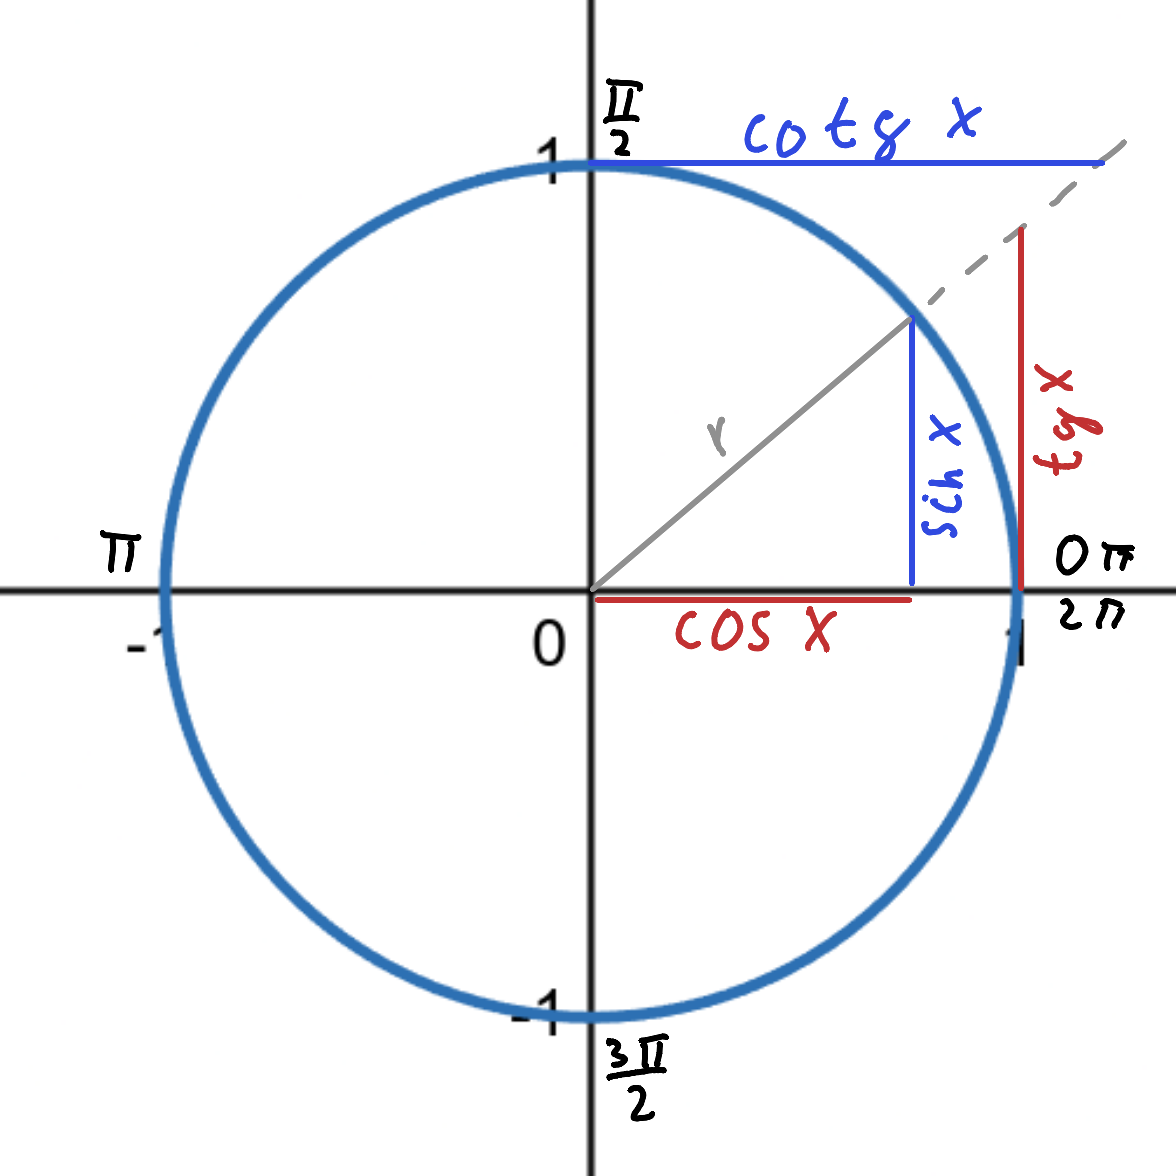
\includegraphics[width=0.6\linewidth]{img/7_JednotkovaKruznice.png}
        \caption{Jednotková Kružnice} 
        \label{fig:Jednotková Kružnice}
\end{figure}
Funkce jsou periodické, což znamená, že se jejich hodnoty pravidelně opakují (jako na kruhu)
\subsection{Grafy funkcí}
\subsubsection{Sinus a Kosinus}
\begin{figure}[H]
        \centering
        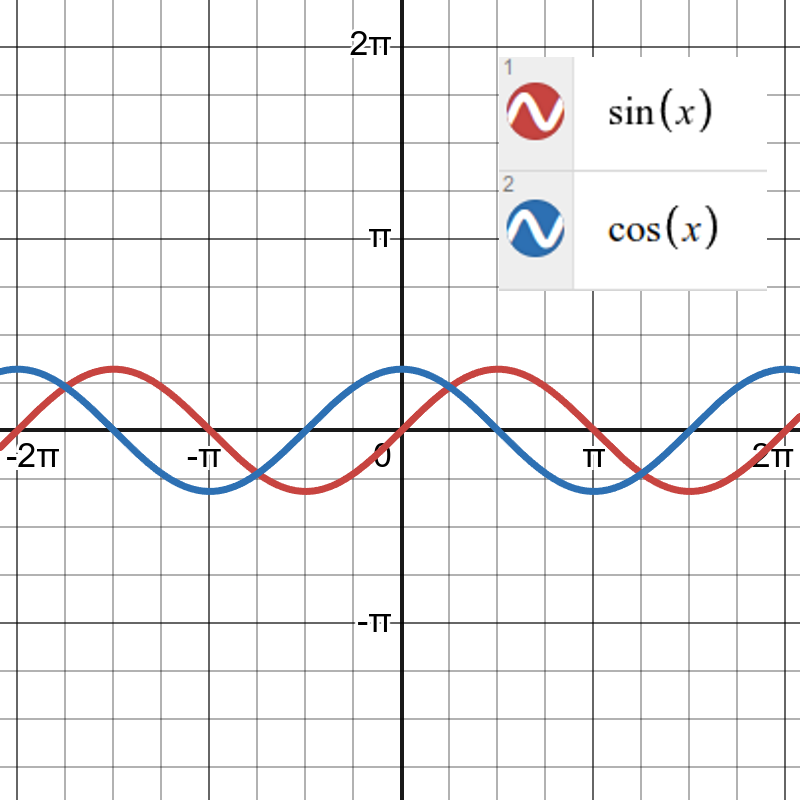
\includegraphics[width=0.5\linewidth]{img/7_SinXCosX.png}
        \caption{$f(x): y=sin(x), g(x): y=cos(x)$} 
        \label{fig:Graf rovnice sin(x) a cos(x)}
\end{figure}

sin(x) začíná v počátku, tedy v bodě [0;0] (na grafu znázorněn červeně). Je to lichá funkce (souměrná podle počátku, jako jediná goniometrická funkce)  periodická v intervalu $\langle0; 2\pi\rangle$. Je definována v pravoúhlém trojúhelníku, jako poměr délky protilehlé odvěsny úhlu alfa ku délce přepony:
$$
    \sin\alpha=\frac{\text{délka protilehlé odvěsny úhlu alfa}}{\text{délka přepony}}
$$
\begin{figure}[h]
    \centering
    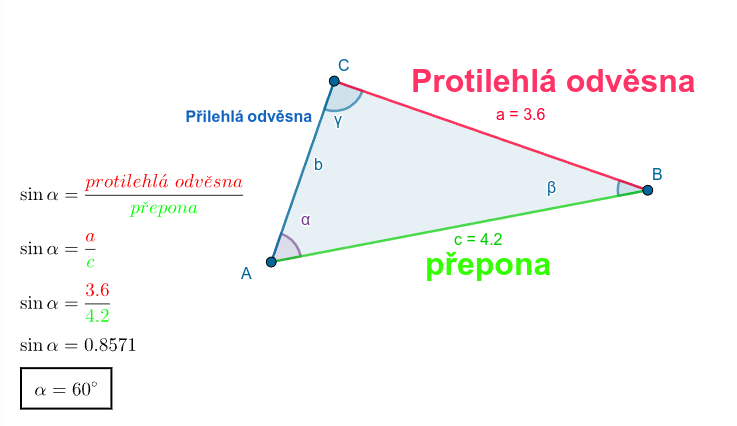
\includegraphics[width=0.5\linewidth]{img/7_TrojuhlenikASinus.png}
    \caption{$\sin \alpha$, znázorněn na pravoúhlém trojúhelníku}
    \label{fig:sinus-na-pravouhlem-trojuhelniku}
\end{figure}
cos(x) začíná v bodě [0;1] (na grafu znázorněn modře), je  to sudá funkce (souměrná podle osy x) a periodická v intervalu $\langle0; 2\pi\rangle$. Je definována v pravoúhlém trojúhelníku, jako poměr délky přilehlé odvěsny úhlu alfa ku délce přepony:
$$
    \cos\alpha=\frac{\text{délka přilehlé odvěsny úhlu alfa}}{\text{délka přepony}}
$$
\begin{figure}[h]
    \centering
    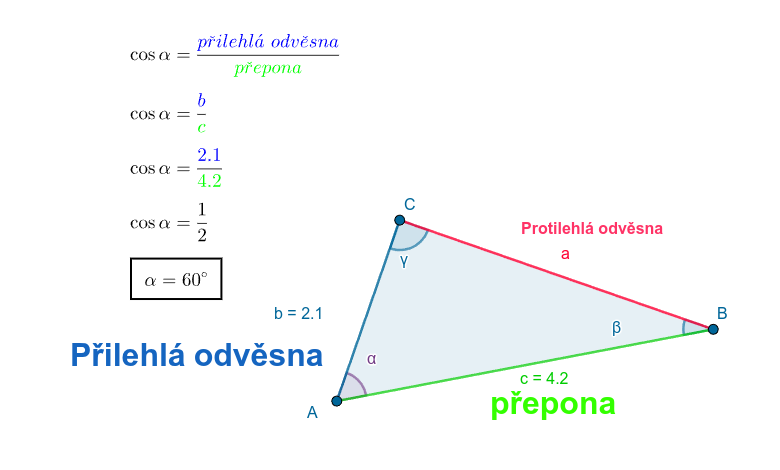
\includegraphics[width=0.5\linewidth]{img/7_TrojuhlenikAKosinus.png}
    \caption{$\cos \alpha$, znázorněn na pravoúhlém trojúhelníku}
    \label{fig:kosinus-na-pravouhlem-trojuhelniku}
\end{figure}
\subsubsection{Tangens a Kotangens}
\begin{figure}[H]
        \centering
        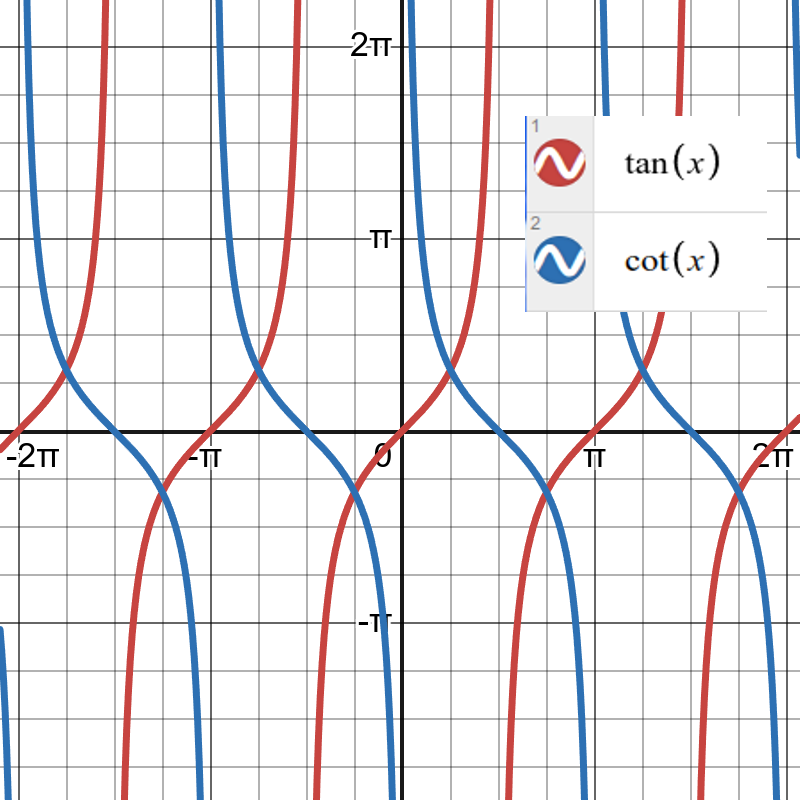
\includegraphics[width=0.5\linewidth]{img/7_TgXCotgX.png}
        \caption{$f(x): y=tg(x), g(x): y=cotg(x)$} 
        \label{fig:Graf rovnice tg(x) a cotg(x)}
\end{figure}

tg(x), na grafu červeně, je funkce periodická v intervalu $\pi$ (o polovinu méně než sin(x) a cos(x)), lichá, definovaná v intervalu $(-\frac{\pi}{2};\frac{\pi}{2})$ je definována jako poměr:
$$
    tg(x) = \frac{\sin(x)}{\cos(x)}
$$
V pravoúhlém trojúhelníku odpovídá poměru délky protilehlé odvěsny ku přilehlé odvěsně:
$$
    tg(x) = \frac{\text{protilehlá odvěsna}}{\text{přilehlá odvěsna}}
$$
Tangens není definován pro ty úhly, kdy je $\cos(x) = 0$, takže \textbf{neexistuje} $tg\left(\frac{\pi}{2} + k\pi\right)$, neboli $90^{\circ}+ k \times 180^{\circ}$ kde $k \in \mathbb{Z}$. 

\begin{figure}[h]
    \centering
    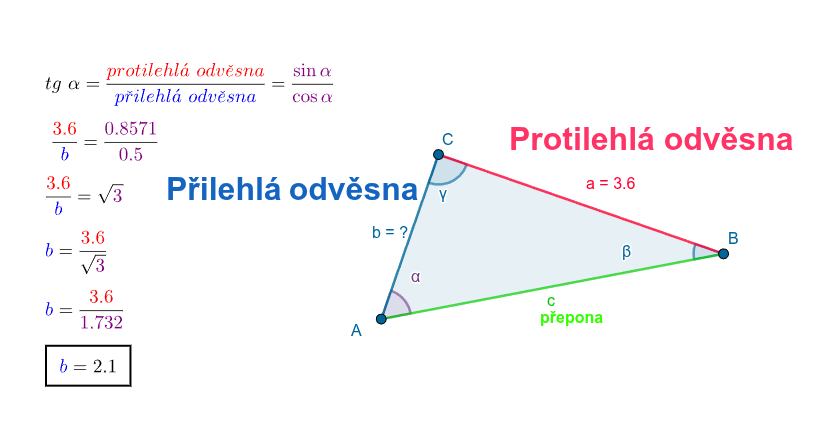
\includegraphics[width=0.5\linewidth]{img/7_TrojuhlenikATangens.png}
    \caption{$tg\ \alpha$, znázorněn na pravoúhlém trojúhelníku}
    \label{fig:tangens-na-pravouhlem-trojuhelniku}
\end{figure}

cotg(x), na grafu modře, je taktéž periodická funkce s periodou $\pi$, a je definována jako poměr:
$$
    cotg(x) = \frac{\cos(x)}{\sin(x)}
$$
V pravoúhlém trojúhelníku představuje poměr délky přilehlé odvěsny ku protilehlé odvěsně:
$$
    cotg(x) = \frac{\text{přilehlá odvěsna}}{\text{protilehlá odvěsna}}
$$
Kotangens není definován pro ty úhly, kdy je $\sin(x) = 0$, takže \textbf{neexistuje} $cotg(k\pi)$, neboli $0^{\circ}+ k \times 180^{\circ}$ kde $k \in \mathbb{Z}$
\begin{figure}[h]
    \centering
    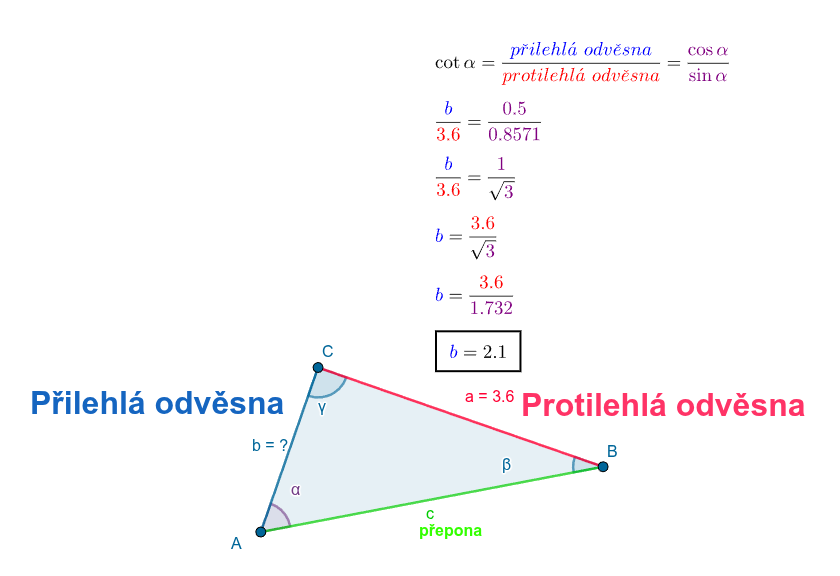
\includegraphics[width=0.5\linewidth]{img/7_TrojuhlenikAKotangens.png}
    \caption{$cotg\ \alpha$, znázorněn na pravoúhlém trojúhelníku}
    \label{fig:kotangens-na-pravouhlem-trojuhelniku}
\end{figure}
\subsection{Tabulky}
\begin{table}[h]
    \centering
    \begin{tabular}{|c|c|c|c|c|c|}
        \hline
        \multicolumn{2}{|c|}{\textbf{ÚHLY}} & \multicolumn{4}{c|}{\textbf{GON. FUNKCE}} \\ \hline
        $\alpha^\circ$ & $\alpha$ (rad) & $\sin \alpha$ & $\cos \alpha$ & $\tan \alpha$ & $\cot \alpha$ \\ \hline
        $30^\circ$ & $\frac{\pi}{6}$ & $\frac{1}{2}$ & $\frac{\sqrt{3}}{2}$ & $\frac{\sqrt{3}}{3}$ & $\sqrt{3}$ \\ \hline
        $45^\circ$ & $\frac{\pi}{4}$ & $\frac{\sqrt{2}}{2}$ & $\frac{\sqrt{2}}{2}$ & 1 & 1 \\ \hline
        $60^\circ$ & $\frac{\pi}{3}$ & $\frac{\sqrt{3}}{2}$ & $\frac{1}{2}$ & $\sqrt{3}$ & $\frac{\sqrt{3}}{3}$ \\ \hline
    \end{tabular}
    \caption{Hodnoty  goniometrických funkcí}
    \label{tab:Goniometricke_Funkce}
\end{table}

\begin{table}[h]
    \centering
    \begin{tabular}{|c|c|c|c|c|}
    \hline
    \textbf{Kvadrant} & sin(x) & cos(x) & tg(x) & cotg(x) \\ \hline
    I.  & + & + & + & + \\ \hline
    II. & + & -- & -- & -- \\ \hline
    III.& -- & -- & + & + \\ \hline
    IV. & -- & + & -- & -- \\ \hline
    \end{tabular}
    \caption{Tabulka znamének pro kvadranty}
    \label{tab:Znamenka_Goniometrie}
\end{table}
\subsection{Jak na to?}
\subsubsection{Sinus a Kosinus}
Je dobré pro orientaci použít jednotkovou kružnici, jde to udělat i bez ní, ale pokud se opravdu chcete vyhnout chybě, tak se hodí. Jako jednoduchý příklad jsem použil hodnotu $\sin(x) = \frac{1}{2}$.
\begin{enumerate}
    \item Hledáme všechny hodnoty $x$, pro které platí $\sin(x) = \frac{1}{2}$.
    
    \item Teď se podíváme do tabulky, z toho zjistíme že pro $\frac{1}{2}$ je $\sin{\frac{\pi}{6}}$:
    \[
    \sin\left(\frac{\pi}{6}\right) = \frac{1}{2}
    \]
    To znamená, že jeden z úhlů, který tuto rovnici splňuje, je $\frac{\pi}{6}$.

    \item ALE funkce sinus je kladná i ve druhém kvadrantu, existuje ještě druhý úhel s touto hodnotou, jak je vidět na jednotkové kružnici:
    \begin{figure}[H]
        \centering
        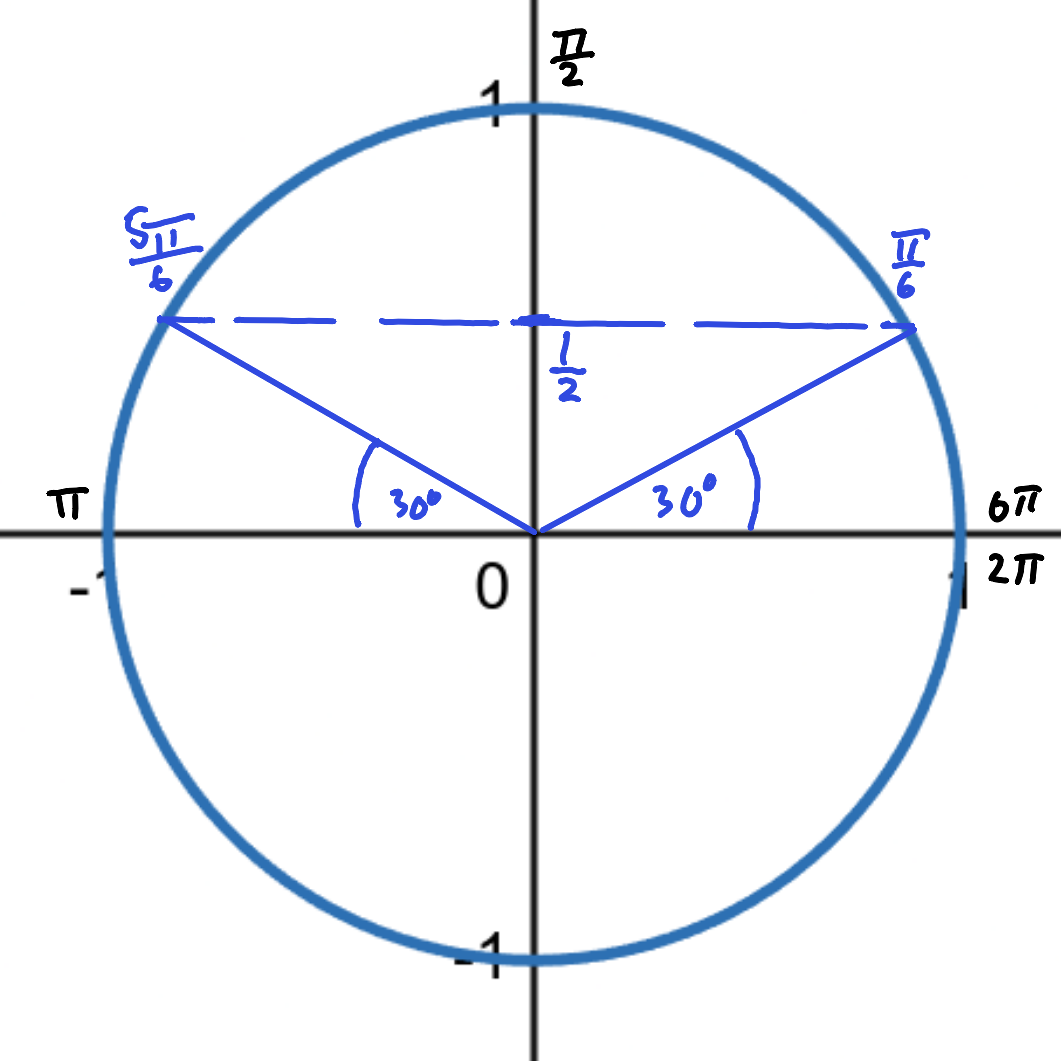
\includegraphics[width=0.4\linewidth]{img/7_JednotkovaKruzniceSinpolovina.png}
        \caption{$\sin{\frac{1}{2}}$} 
        \label{fig:Sinus jedné poloviny na jednotkové kružnici}
\end{figure}
    \[
    x = \pi - \frac{\pi}{6} = \frac{5\pi}{6}
    \]

    \item Funkce sinus je periodická s periodou $2\pi$, takže obecné řešení je:
    \[
    x_1 = \frac{\pi}{6} + 2k\pi \quad, \quad x_2 = \frac{5\pi}{6} + 2k\pi, \quad k \in \mathbb{Z}
    \]
\end{enumerate}
V případě že počítáme funkci $cos(x)$, postup je stejný, jediný rozdíl je, že místo osy $y$ použijeme osu $x$, a to takto:
\begin{figure}[H]
        \centering
        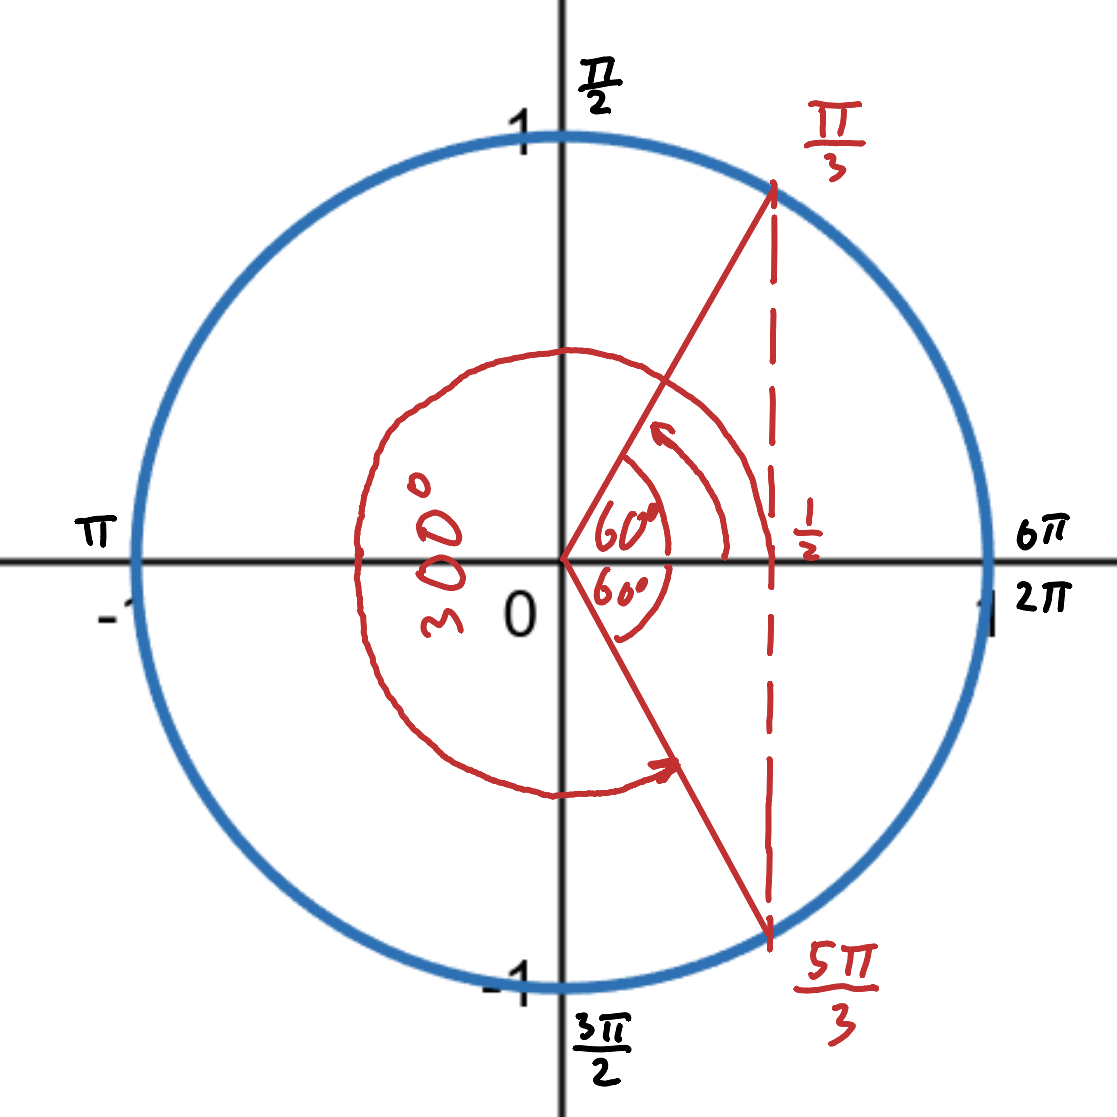
\includegraphics[width=0.4\linewidth]{img/7_JednotkovaKruznicekosinuspolovina.png}
        \caption{$\cos{\frac{1}{2}}$} 
        \label{fig:Kosinus jedné poloviny na jednotkové kružnici}
\end{figure}
\subsubsection{Tangens a Kotangens}
Tito dva se zdají být výrazně děsivější, ale jakmile to pochopíte, je to vcelku jednoduché, tady je příklad s tabulkovou hodnotou:
\begin{enumerate}
    \item Hledáme hodnoty $x$, pro které platí $\tan(x) = \sqrt{3}$.

    \item Když se podíváme to tabulky, zjistíme že:
    \[
    \tan\left(\frac{\pi}{3}\right) = \sqrt{3}
    \]
    Takže jeden z úhlů, který tuto rovnici splňuje, je:
    \[
    x = \frac{\pi}{3}
    \]
    \begin{figure}[H]
        \centering
        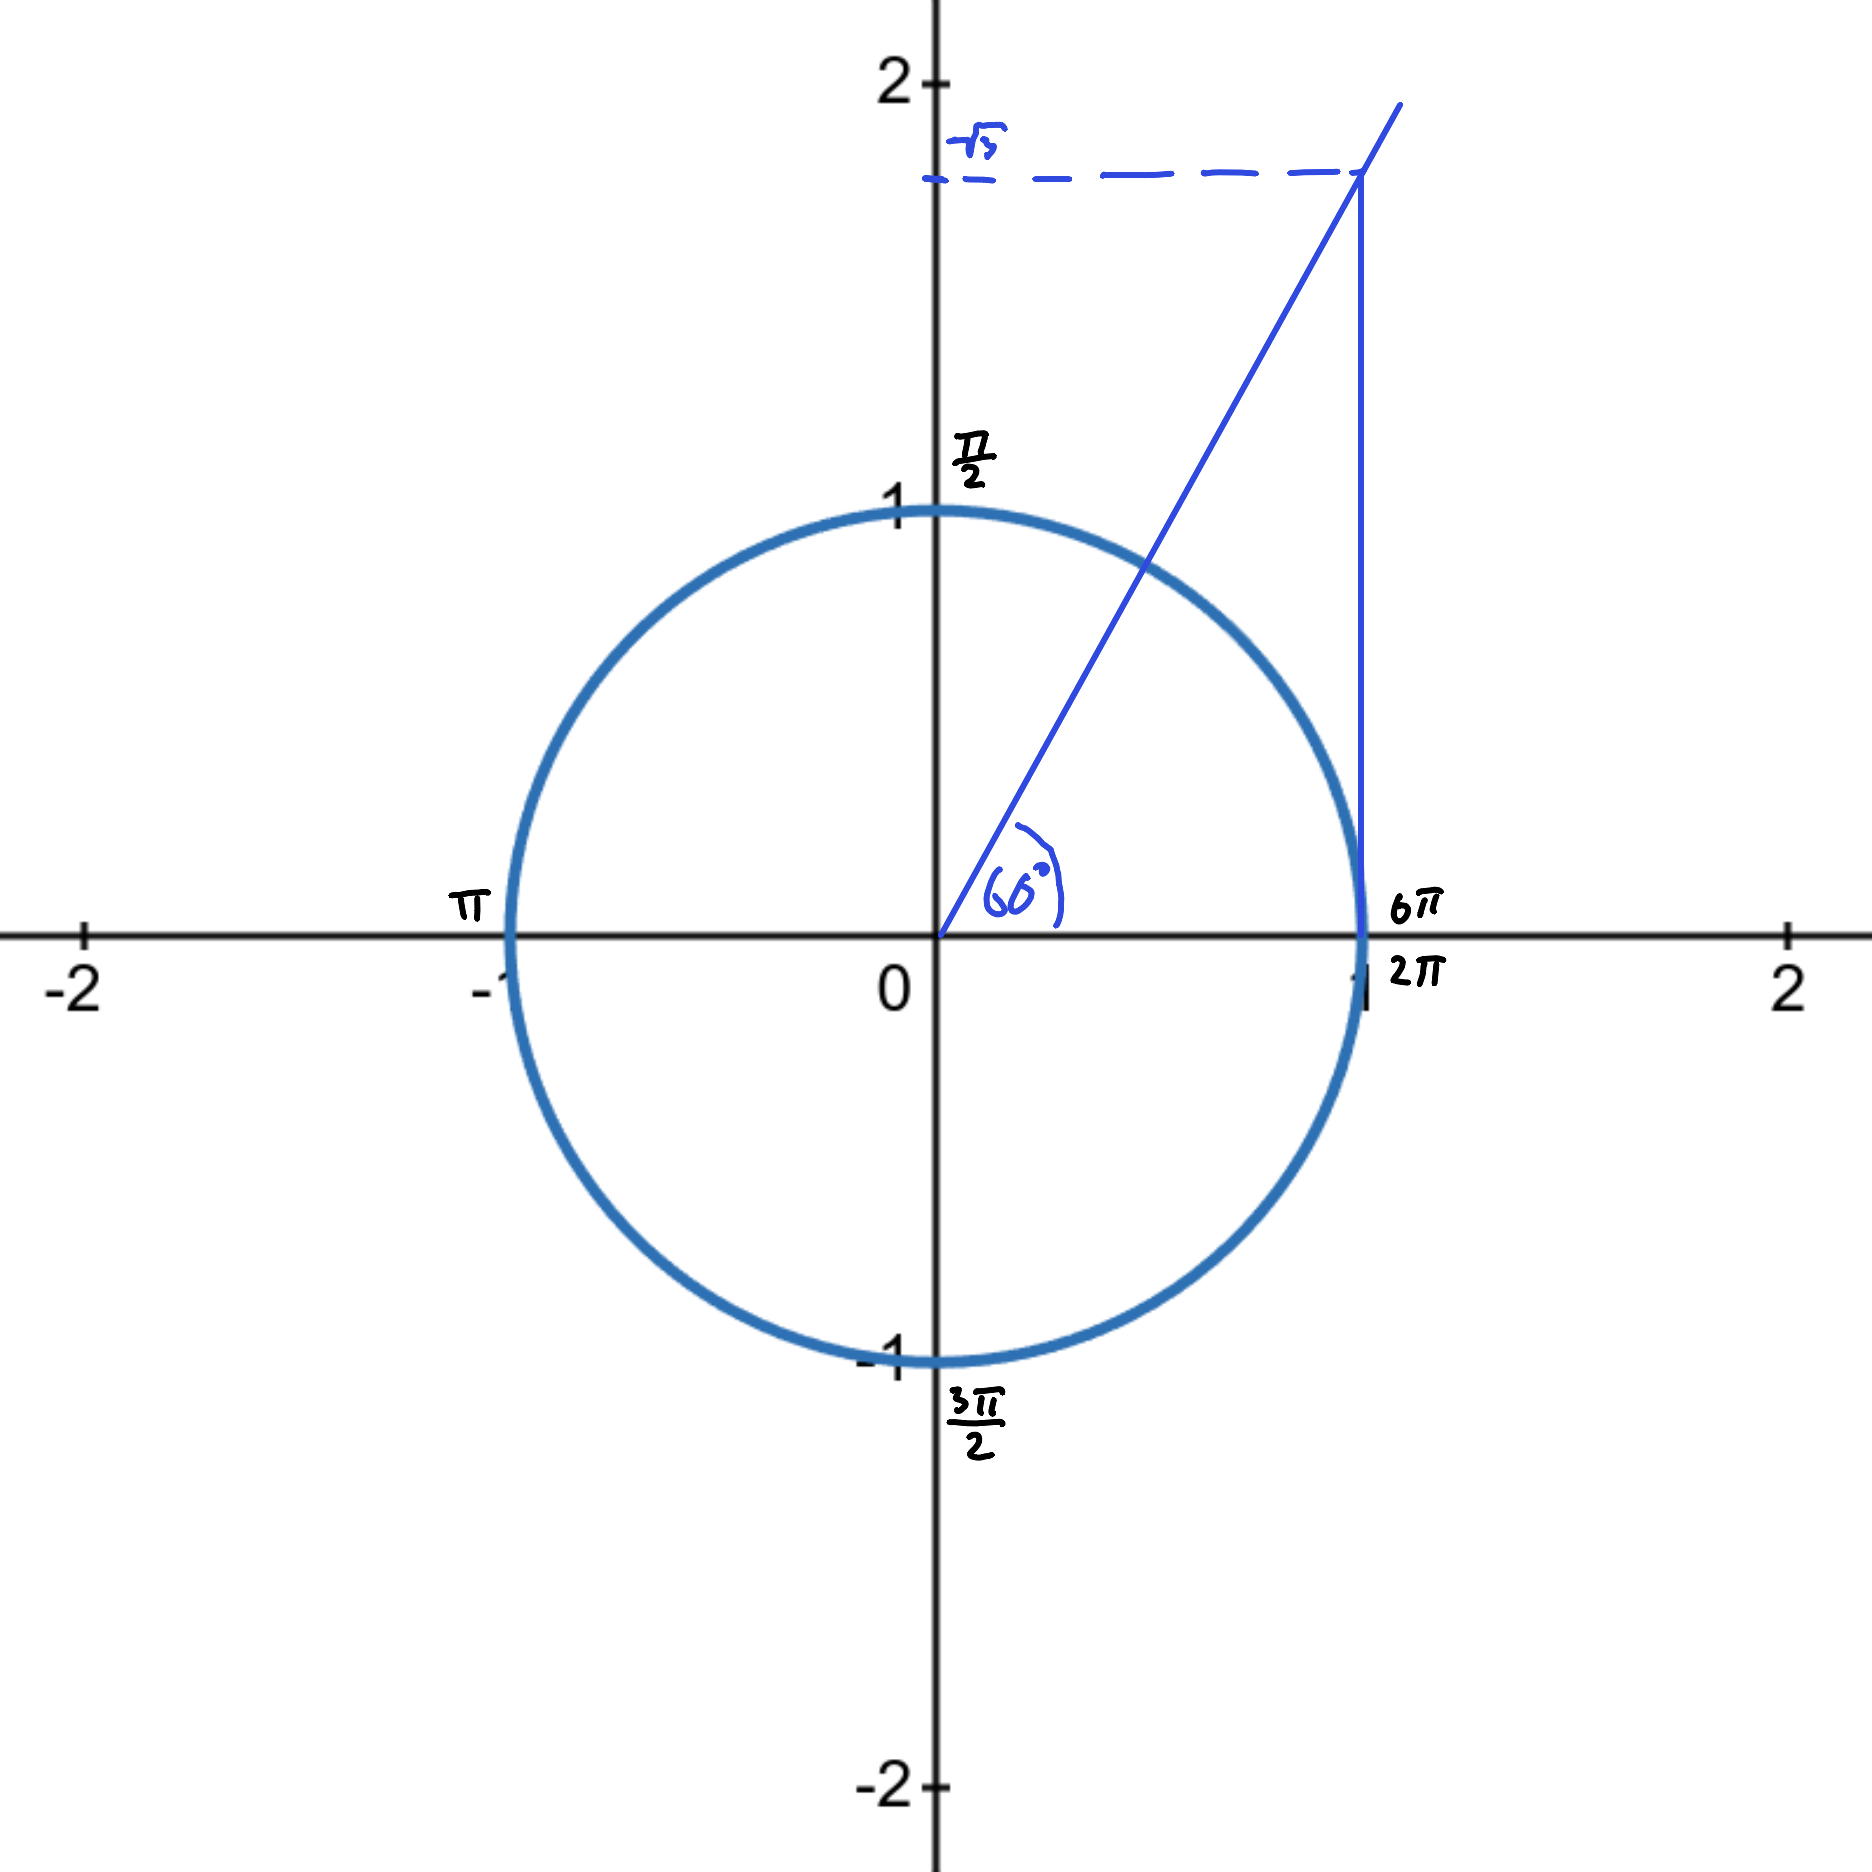
\includegraphics[width=0.5\linewidth]{img/7_JednotkovaKruzniceTangens.png}
        \caption{$tg\sqrt{3}$} 
        \label{fig:Tangens jedné poloviny na jednotkové kružnici}
\end{figure}

    \item Funkce tangens má periodu $\pi$, protože se opakuje každých 180° (ne každých $2\pi$ jako sinus a kosinus), také je na rozdíl od nich kladný v protilehlých kvadratech, tedy v prvním a třetím kvadrantu. O to je naše práce jednoduší, jak jsem znázornil na jednotkové kružnici, stačí pouze z naši polopřímku protáhnout na druhou stranu.
%Tento obrázek může klidně být místo toho prvního, poté by se to všechno vlezlo na stránku, je na tobě jestli si myslíš, že to tady je dobré nechat.
    \begin{figure}[H]
        \centering
        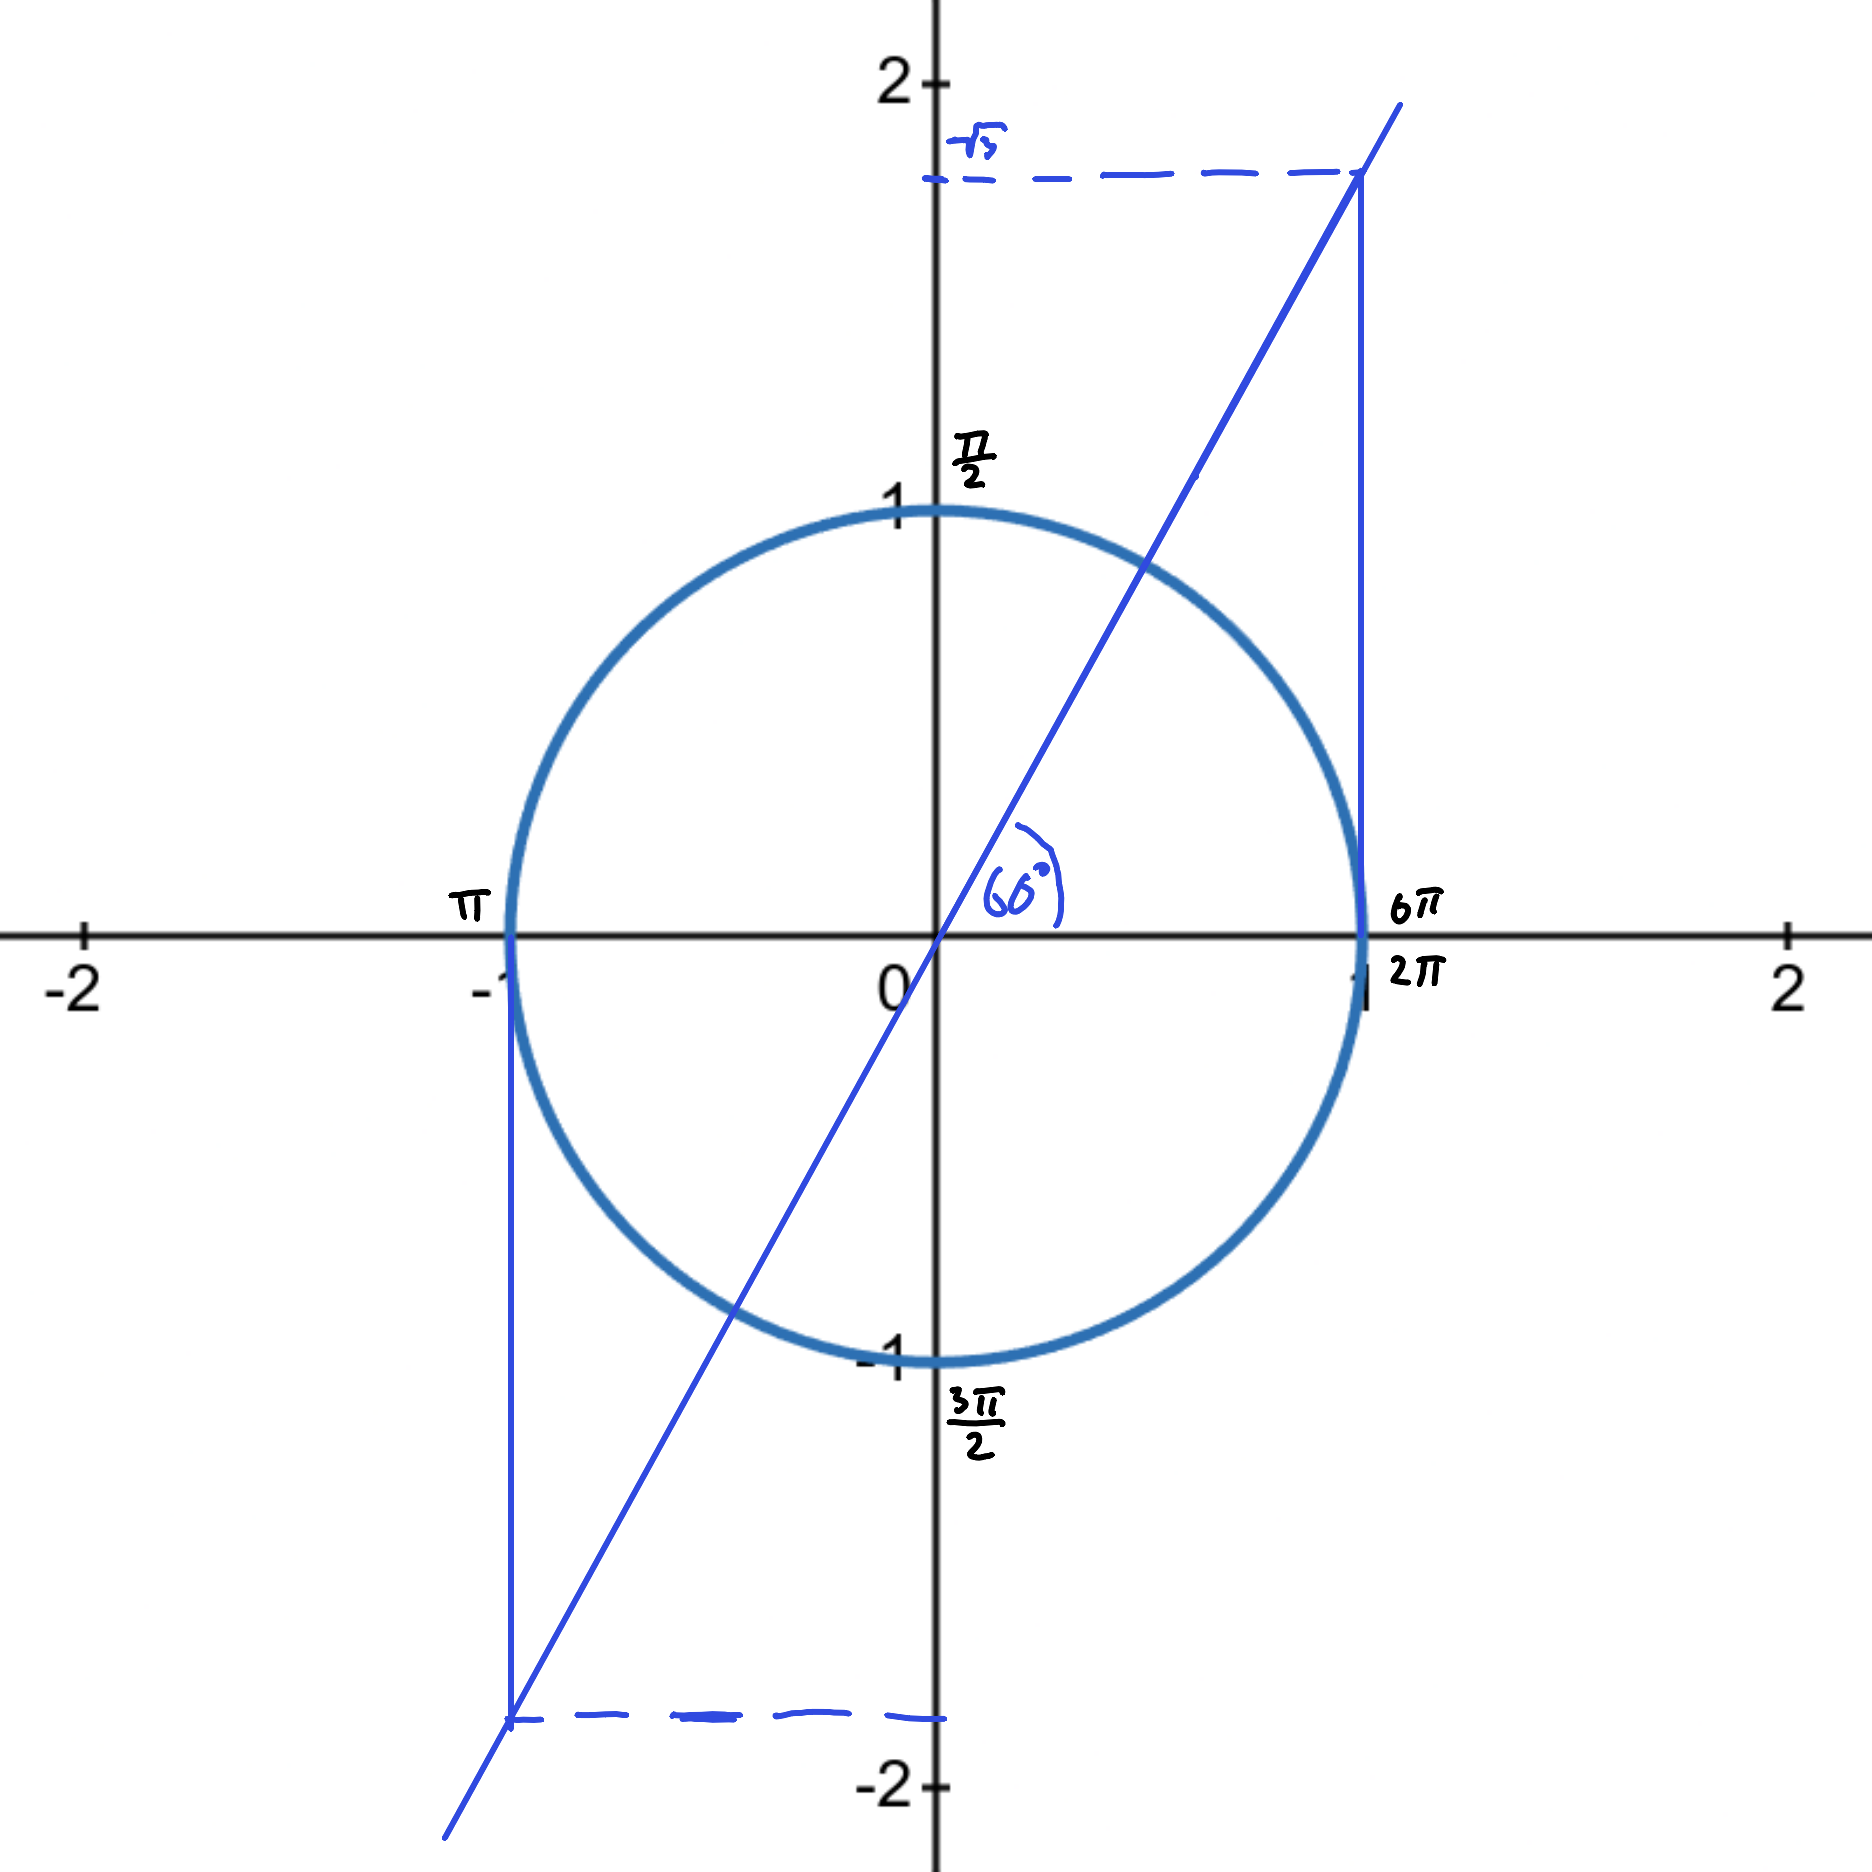
\includegraphics[width=0.5\linewidth]{img/7_JednotkovaKruzniceTangensKomplet.png}
        \caption{$tg\sqrt{3}$} 
        \label{fig:Tangens jedné poloviny na jednotkové kružnici, dokončeno}
    \end{figure}
    \item Taky je dobré si všimnout, že $\sqrt{3} > 1$, toto je možné pouze proto, že $tg(x)$ a $cotg(x)$ mohou dosahovat $-\infty$ až $+\infty$, vyjma tedy těch hodnot, kdy by hodnota ve jmenovateli byla rovna $0$.

    \item Obecné řešení rovnice tedy je:
    \[
    x = \frac{\pi}{3} + k\pi, \quad k \in \mathbb{Z}
    \]

\end{enumerate}
V případě funkce $cotg(x)$ je to podobné jako u kosinu.
\title{8 Goniometrické rovnice}
\author{Roman Šnajder}
\date{May 2025}


\maketitle

\section{Goniometrické rovnice}
\subsection{Základní goniometrické rovnice}
Rovnice v nichž se vyskytují goniometrické výrazy s neznámou $x\in R$ nazýváme goniometrické rovnice. Vzhledem k tomu, že jsou goniometrické funkce periodické, mohou mít goniometrické rovnice nekonečně mnoho kořenů. Stačí za k v $k\pi$ dosadit jakékoliv celé číslo.
$$\sin(x)=\frac{1}{2}$$
$$x=\frac{\pi}{6}$$
$$x_1=\frac{\pi}{6}+2k\pi$$
$$x_1=\frac{5\pi}{6}+2k\pi$$
Rovnice, ve kterých funkce nabývají hodnot mimo interval $\langle -1; 1 \rangle$ nemají řešení, jelikož se tato čísla nenacházejí na jednotkové kružnici. Například $\sin(x)=3$.
Tato rovnice $3\sin(x)=2$ však řešení má, jelikož jde obě strany vydělit číslem $3$ a dostaneme $\sin(x)=\frac{2}{3}$.
\subsection{Použití substituce u goniometrických rovnic}
$$2\sin(x)^2+\sin(x)-1=0$$ $$\sin(x)=t$$
$$2t^2+t-1=0$$
$$(t+1)\cdot(2t-1)=0$$
$$t_1=-1; t_2=\frac{1}{2}$$
$$\sin(x)=-1;\sin(x)=\frac{1}{2}$$
$$x_1=\frac{3}{2}+2k\pi$$
$$x_2=\frac{\pi}{6}+2k\pi;x_3=\frac{5\pi}{6}+2k\pi$$
Substituci lze využít i takto:
$$\sin(2x-\frac{\pi}{3})=1$$
$$2x-\frac{\pi}{3}=t$$
$$\sin(t)=1$$
$$t=\frac{\pi}{2}+2k\pi$$ 
$$2x-\frac{\pi}{3}=\frac{\pi}{2}+2k\pi$$
$$2x=\frac{5\pi}{6}+2k\pi$$
$$x=\frac{5\pi}{12}+k\pi$$
Goniometrické rovnice je možné řešit i za pomoci následujících vzorečků (zde jsou vypsány pouze některé vzorce):
$$\sin^2x+\cos^2x=1$$
$$tgx=\frac{\sin(x)}{\cos(x)}$$
$$cotgx=\frac{\cos(x)}{\sin(x)}$$
$$tgx-cotgx=1$$
$$\sin2x=2\cdot \sin(x)\cdot \cos(x)$$
$$\cos(2x)=\cos^2x-\sin^2x$$
\subsection{Kvadranty}
Každou goniometrickou funkci, která je definována v $\langle0; 2\pi\rangle$ lze znázornit na jednotkové kružnici, kde mezi každými dvěma osami je právě jeden kvadrant. V celku je tedy kružnice tvořena čtyřmi kvadranty a pomocí jedné hodnoty $(\frac{\pi}{6})$ v obloukové míře je možné dopočítat hodnoty ve zbylých kvadrantech $(\frac{5\pi}{6}); (\frac{7\pi}{6}); (\frac{11\pi}{6})$ opět v obloukových mírách.
Zde jsou pravidla pro výpočet daných hodnot $$x_1=x_0$$ $$x_2=\pi-x_0$$ $$x_2=\pi+x_0$$ $$x_2=2\pi-x_0$$
\subsubsection{Jednotková kružnice}
Vzdálenost od středu se vypočítá jako tangens úhlu nebo poměr protilehlé strany (sin osy y) ku přilehlé straně (cos osy x). V pravoúhlém trojúhelníku může tangens úhlu dosahovat libovolných kladných hodnot. Pohyb na grafu od $(0;\infty)$ se na jednotkové kružnici znázorní pohybem PROTI SMĚRU hodinových ručiček.
\begin{itemize}
    \item Funkce sinus v prvních dvou kvadrantech je kladná, v druhých dvou je záporná
    \item Funkce cosinus v prvním a čtvrtém kvadrantu roste, v druhém a třetím klesá 
    \item Funkce tangens je v první kvadrantu kladná a v druhém záporná
    \item Funkce kotangens je v prvním kvadrantu kladná a v druhém záporná
\end{itemize}
(1. kvadrant vpravo nahoře $(0;90^\circ)$; 2. kvadrant vlevo nahoře $(90^\circ;180^\circ)$; 3. kvadrant vlevo dole $(180^\circ;270^\circ)$; 4. kvadrant vpravo dole $(270^\circ;360^\circ)$)

\begin{figure}
    \centering
    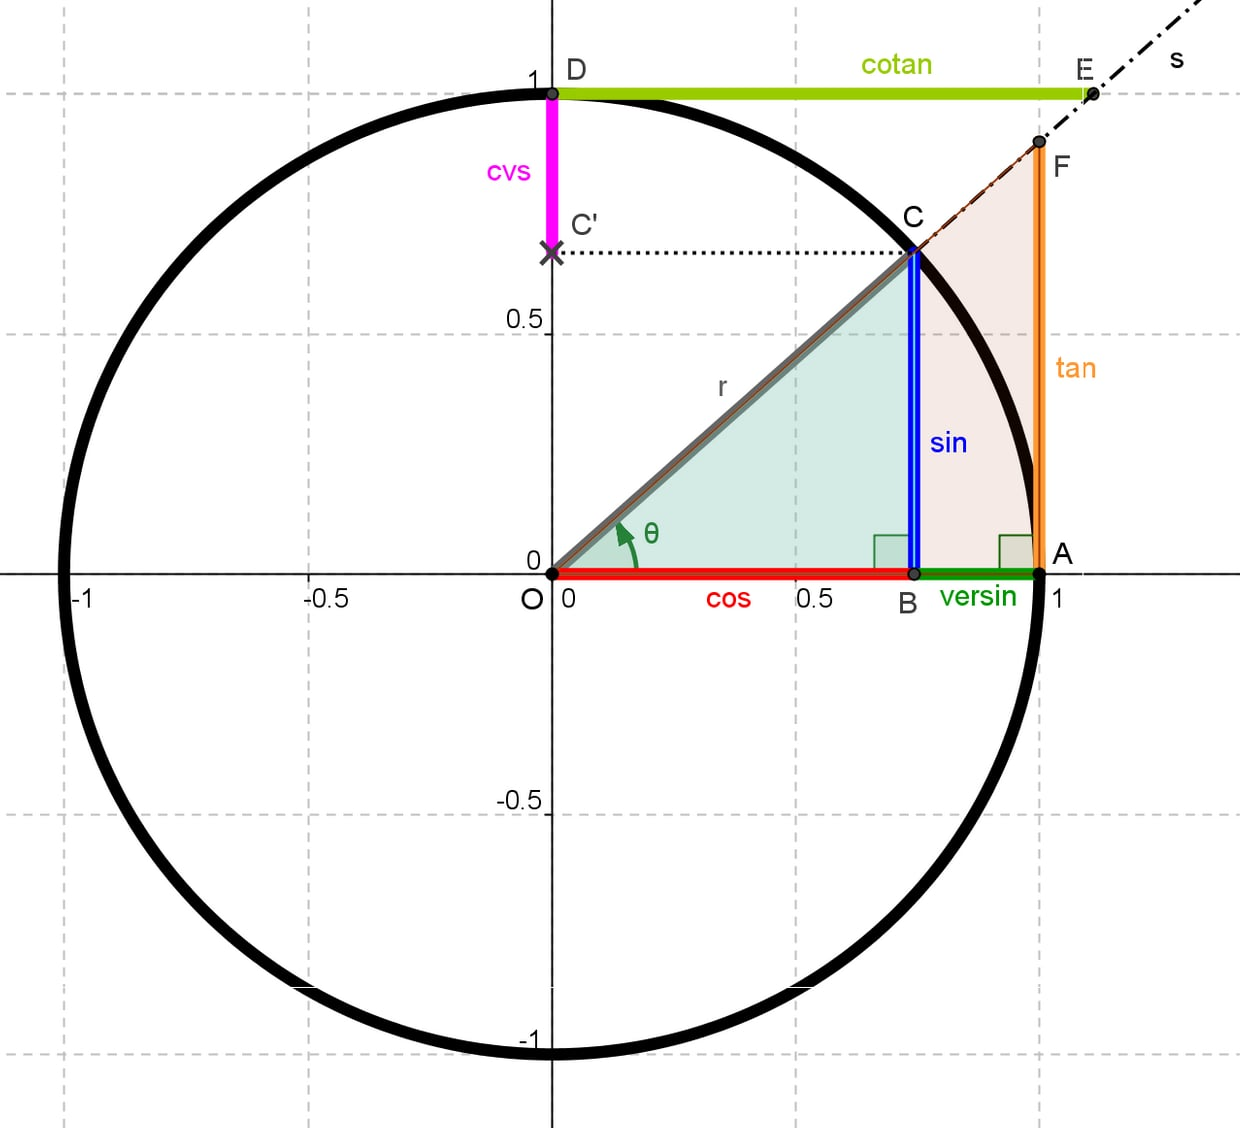
\includegraphics[width=0.5\linewidth]{img/jednotkova_Kruznice.jpg}
    \caption{Jednotková kružnice}
    \label{fig:enter-label}
\end{figure}


\begin{figure}
    \centering
    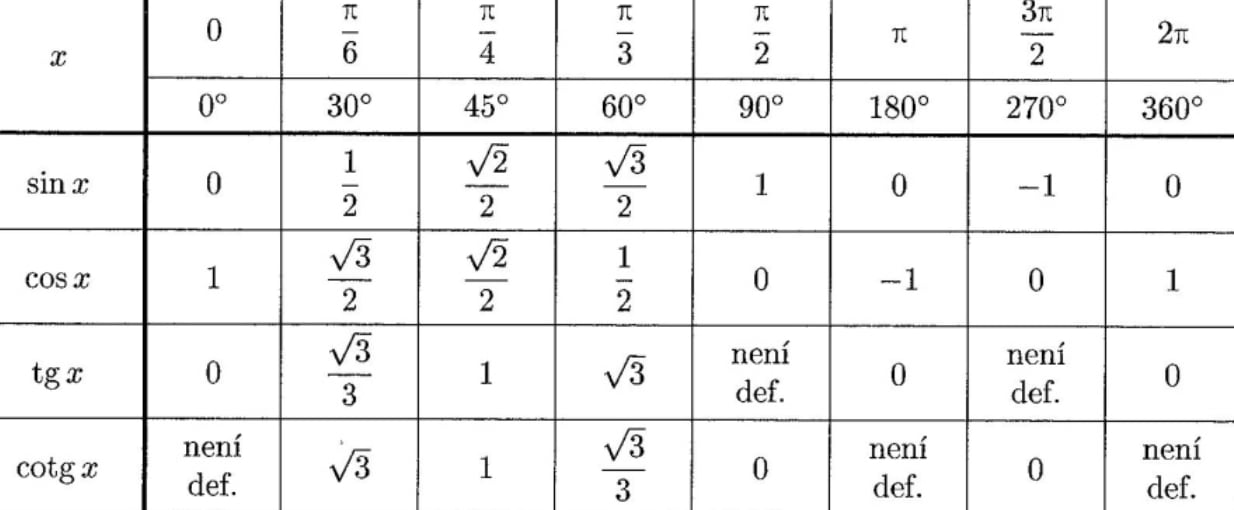
\includegraphics[width=1\linewidth]{img/tabulka_hodnot_goniometrickych.jpg}
    \caption{Tabulka hodnot goniometrických funkcí}
    \label{fig:enter-label}
\end{figure}

\subsection{Řešení rovnice ve stupních a převod mezi radiány a stupni}
Goniometrické rovnice mohu být řešeny buď v radiánech nebo ve stupních – záleží na zadání. Zde jsou vzorečky pro převody mezi stupni a radiány.

\begin{itemize}
    \item Ze stupňů na radiány: $\alpha$ rad=$\frac{\pi}{180\textdegree}\cdot\alpha$ stupně
\\ například $30^\circ$ na radiány
$$
    30^\circ \cdot\frac{\pi}{180^\circ}=\frac{\pi}{6}
$$
    \item Z radiánů na stupně: $\alpha$ stupně=$\frac{180\textdegree}{\pi}\cdot\alpha$ rad
\\ například $\frac{\pi}{2}$ na stupně
$$
    \frac{\pi}{2} \cdot 180^\circ=90^\circ
$$
\end{itemize}

Rovnice zadaná ve stupních $\sin(x)=\frac{\pi}{2}$, $x\in\langle0 ^\circ;360^\circ \rangle$
$$\sin(x)=\frac{\pi}{2} \rightarrow x=30^\circ$$
$$x_1=30$$
$$x_2=180^\circ-30^\circ\Rightarrow150^\circ$$
\subsection{Řešení rovnice v daném intervalu}
Pokud je goniometrická rovnice zadána s konkrétním intervalem, musí být řešena právě v tomto intervalu. Po výpočtu všech možných řešení je nutné tato řešení porovnat s daným intervalem a zapsat pouze ta, která do něj skutečně náleží.
Rovnice $cosx=-\frac{\pi}{2}$, $x\in\langle\frac{\pi}{2};\frac{3\pi}{2}\rangle$
$$x_1=\pi-\frac{\pi}{3}\Rightarrow\frac{2\pi}{3}$$
$$x_2=\pi+\frac{\pi}{3}\Rightarrow\frac{4\pi}{3}$$

\include{9_Komplexni_císla}
\title{ 10. Kombinatorika}
\author{Marek Fuchs (Oliver Hadraba)}
\date{26.4.2025}

\maketitle



\section{Kombinatorika}
    
     \subsection{Faktoriál}
     Faktoriál čísla $n$ je roven součinu všech přirozených čísel $N$ $(1;2;3;..)$, která jsou menší nebo rovna číslu $n$.\\
     Faktoriál zapisujeme pomocí vykřičníku $\rightarrow{n!}$\\
    Například: $5! = 5\cdot4\cdot3\cdot2\cdot1=120$
     
     \subsection{Variace}
     Variace k-té třídy z $n$ prvků je každá uspořádaná k-tice vytvořená z celkového počtu $n$ prvků, přičemž při výběru záleží na pořadí jednotlivých prvků.
     \begin{itemize}
         \item Bez opakování
         $$
         V_k (n)=\frac{n!}{(n-k)!}
         $$
         \item S opakováním
         $$
         V_k (n)=n^k
         $$
     \end{itemize}
Například: Vybíráme 4 studenty z 25 na zkoušení a záleží jim na tom, kolikátí budou vybráni, aby se mohli učit co nejdéle. V tomto případě záleží na pořadí a proto pro výpočet počtu možností použijeme variace. 

     \subsection{Permutace}
     Kolika způsoby lze uspořádat všechny $n$ prvky.\\
     Permutace je zvláštní případ variace, kde $k=n$. To znamená, že ze zadaných prvků postupně vybereme všechny. Každá permutace tedy odpovídá nějakému pořadí zadaných prvků: každý prvek se v pořadí musí objevit, ale žádný tam nemůže být dvakrát. Permutace z $n$ prvků je každá n-členná variace z těchto prvků.
     $$
     P(n)=n!
     $$
     $$
     P(n)=n \cdot(n-1)\cdot(n-2) \ ...2\cdot1=n!
     $$
     Případ, kdy zkoušíme všechny studenty.
     \subsection{Kombinace}
     Kombinace je neuspořádaná k-tice vytvořená z celkového počtu $n$ prvků, přičemž nezáleží na pořadí vybraných prvků.
     \begin{itemize}
         \item Bez opakování
         $$
         C_k (n)= {n \choose k}=\frac{n!}{k!(n-k)!}
         $$
         Využíváme například, pokud vybíráme z 6 kluků 3, kteří budou současně zametat (nezáleží na pořadí v kterém budou vybráni)
         \item S opakováním
         $$
         C_k(n)= {n+k-1 \choose k}
         $$
     \end{itemize}
     
     \subsection{Kombinační číslo}
     \textbf{Kombinační číslo}, označované jako $\binom{n}{k}$ (čteme: n nad k), udává počet způsobů, jak lze z množiny $n$ prvků vybrat právě $k$ prvků bez ohledu na pořadí.

Matematicky je definováno jako:

\[
\binom{n}{k} = \frac{n!}{k!(n-k)!}, \quad \text{pro } 0 \leq k \leq n
\]

kde $n!$ značí \textit{faktoriál} čísla $n$, tedy součin všech přirozených čísel od $1$ do $n$.

Pro $k > n$ platí:

\[
\binom{n}{k} = 0
\]
     \subsection{Binomická věta}
     Binomická věta říká, že:
     $$
        (a + b)^n = \sum_{k=0}^{n} \binom{n}{k} a^{n-k} b^k
     $$
     Znamená to, že výraz $(a + b)^n$ se rozepíše jako součet členů, ve kterých:

\begin{itemize}
  \item mocniny $a$ a $b$ se vždy doplňují do $n$,
  \item koeficienty jsou \textbf{binomické koeficienty}: 
  \[
  \binom{n}{k} = \frac{n!}{k!(n-k)!},
  \]
  \item index $k$ určuje, kolikrát se v daném členu vyskytuje $b$, a tedy i kolikrát $a$.
\end{itemize}

\subsubsection{Příklad pro $n = 3$}

\[
(a + b)^3 = \binom{3}{0}a^3b^0 + \binom{3}{1}a^2b^1 + \binom{3}{2}a^1b^2 + \binom{3}{3}a^0b^3
\]

\[
= 1 \cdot a^3 + 3 \cdot a^2b + 3 \cdot ab^2 + 1 \cdot b^3
\]

\[
= a^3 + 3a^2b + 3ab^2 + b^3
\]
\\
     Při řešení různých algebraických úloh potřebujeme občas umocnit dvojčlen $a+b$ na přirozené číslo $n$, tj. vypočítat $(a+b)^n$.\\
     Když chceme určit k-tý člen binomického rozvoje použijeme tento vzoreček:
     $$
     (a+b)^n={n \choose k-1}\cdot a^{n-(k-1)}\cdot b^{k-1}
     $$
     Příklad:\\
     Určete čtvrtý člen výrazu $(x+2)^{12}$
     $$
     (x+2)^{12}={12 \choose 3}\cdot x^9\cdot 2^3=220\cdot x^9 \cdot8=1760x^9
     $$
     \subsection{Pascalův trojúhelník}
     Je tvořen čísly a platí, že číslo, které se nachází pod jinými dvěma čísly, se rovná jejich součtu.\\
     \\

\begin{figure}[H]
        \centering
        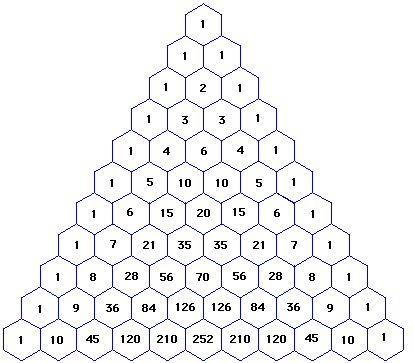
\includegraphics[width=0.4\linewidth]{img/21_pascaluvTrojuhelnik1_realny.jpg}
        \caption{Pascalův trojúhelník s přirozenými čísly} 
        \label{fig:enter-label}
    \end{figure}

\begin{figure}[H]
        \centering
        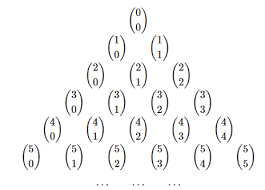
\includegraphics[width=0.4\linewidth]{img/21_paskal_kombinacni_cisla.png}
        \caption{Pascalův trojúhelník s kombinačními čísly} 
        \label{fig:enter-label}
    \end{figure}
    
     
\subsection{Výpočet rovnice}
Upravme výraz:
\[
\frac{1}{n!} - \frac{3}{(n+1)!}
\]

Společný jmenovatel je $(n+1)! = (n+1) \cdot n!$:

\[
= \frac{(1)(n+1) - 3}{(n+1)!} = \frac{n - 2}{(n+1)!}
\]

\subsection{Speciální případy kombinačních čísel}
     \begin{itemize}
         \item $k=0$
         $$
         {n \choose 0}=\frac{n!}{0!(n-0)!}=\frac{n!}{n!}=1
         $$
         \item $k=n$
         $$
         {n \choose n}=\frac{n!}{n!(n-n)!}=\frac{n!}{n!}=1
         $$
         \item $k=1$
         $$
         {n \choose 1}=\frac{n!}{1!(n-1)!}=n!
         $$
     \end{itemize}
     \subsection{Vlastnosti kombinačních čísel}
      \begin{itemize}
         \item Pro všechna celá nezáporná čísla $n$, $k$ platí $\rightarrow{k\leq n}$
         $$
         {n \choose n-k}={n \choose k}
         $$
         \item Důkaz:
         $$
         {n \choose n-k}=\frac{n!}{(n-k)![n-(n-k)]!}=\frac{n!}{k!(n-k)!}={n \choose k}
         $$
         \item Tato vlastnost popisuje jednoduchý fakt: Chceme li vybrat k-prvkovou podmnožinu n-prvkové množiny, zbyde vždy $n-k$ nevybraných prvků. Rozhodneme li se tedy vybrat $n-k$ prvků, které do hledaný podmnožiny nezařadíme, počet možností, jak je vybrat bude stejný jako při přímém výběru $k$.
     \end{itemize}
     
\title{11. Posloupnosti}
\author{Kateřina Polášková (Jakub Sláma)}
\date{30.4.2025}

\maketitle

\section{Posloupnosti}
Posloupnost je funkce, jejíž definičním oborem je množina $\mathbb{N}$ (všech přirozených čísel). \\
Posloupnost se nazývá NEKONEČNÁ, pokud je jejím definičním oborem celá množina $\mathbb{N}$.
Posloupnost se nazývá KONEČNÁ, pokud je jejím definičním oborem množina prvních $n$ přirozených čísel ${1, 2, 3, ..., n}$. \\ \\

Funkční hodnoty posloupnosti se nazývají ČLENY POSLOUPNOSTI; funkční hodnota
posloupnosti v bodě $n \in N$ se nazývá nTÝ ČLEN POSLOUPNOSTI a značí se $a_n$. \\ \\

Posloupnost (nekonečnou) zapisujeme $(a_n)^\infty_ {n=1}$, nebo $(a_1,a_2,a_3,.....a_n)$ \\
Konečnou posloupnost zapisujeme $(a_n)^k_{n=1}$ nebo $(a_1,a_2,a_3,.....a_k)$\\
Posloupnost je nejčastěji zadána jedním z těchto dvou způsobů:
\begin{itemize}
    \item Vzorcem, vyjadřujícím n-tý člen posloupnosti pomocí $n$
    \item Rekurentně udáním prvního členu posloupnosti a rekurentního vzorce, který
vyjadřuje $(n + 1)$-ní člen posloupnosti pomocí členů předchozích.
\end{itemize}

\subsection{Definice aritmetické posloupnosti}
ARITMETICKÁ POSLOUPNOST je taková posloupnost, v níž je rozdíl dvou sousedních členů
konstantní. Tento rozdíl $a_{n+1} -a_n $se nazývá DIFERENCE a označuje se $d$, kde $(d \in \mathbb{R})$. \\ \\

Rekurentní vzorec aritmetické posloupnosti je: $a_{n+1}=a_n+d$, kde $n \in \mathbb{N}$\\ \\

Obecný vzorec aritmetické posloupnosti je: $a_n=a_1+(n-1)d$\\
Pro každé dva členy $a_r$, $a_s$ aritmetické posloupnosti platí: $a_r-a_s=(r-s)d$\\
Pro součet prvních $n$ členů aritmetické posloupnosti platí:$s_n=\frac{n}{2}(a_1+a_n)$

\subsection{Definice geometrické posloupnosti}
GEOMETRICKÁ POSLOUPNOST je taková posloupnost, v níž podíl následujícího a předchozího
členu je konstantní. Tento podíl se označuje $q$ a nazývá se KVOCIENT $(q \in \mathbb{R})$.\\
Rekurentní vzorec geometrické posloupnosti je $a_{n+1} = a_n.q$ nebo $\frac{a_{n+1}}{a_n}=q, n\in \mathbb{N}$ \\
Obecný vzorec geometrické posloupnosti je $a_n=a_1 \cdot q^{n-1}$\\
Pro každé dva členy geometrické posloupnosti $a_r, a_s$ platí: $a_r=a_s \cdot q^{r-s}$\\
Pro součet prvních $n$ členů geometrické posloupnosti platí:
$$
    s_n=a_1\frac{q^n-1}{q-1}
$$
pro $q \neq 1$\\
$$
    s_n=n \cdot a_1 
$$ 
pro $ q=1$

\subsection{Důkaz matematickou indukcí}
Dokažte: $\forall\, (n \in \mathbb{N}) :\quad 1 + 2 + \dots + n = \frac{1}{2} \cdot (n + 1) \cdot n$\\ \\

Prvním krokem je ověření platnosti pro číslo 1. Dosadíme tedy toto číslo do rovnosti. Levá strana bude
1, pravá strana bude $\frac{1}{2} \cdot 1 \cdot (1 + 1)$ což je opět 1. Pro číslo 1 tedy věta platí. \\
Přichází na řadu indukční krok. Předpokládejme, že tato věta platí pro nějaké přirozené číslo $k$, tedy že
pro toto $k$ platí:
$$
    1 + 2 + \dots + k = \frac{1}{2} \cdot (k + 1) \cdot k
$$
Nyní musíme dokázat, že za tohoto předpokladu platí věta i pro $(k + 1)$, tedy že platí:
$$
    1 + 2 + \dots + k + (k + 1) = \frac{1}{2} \cdot (k + 2)(k + 1)
$$
Levá strana je $1 + 2 + … k + (k + 1)$. My však z našeho předpokladu víme, že
$1 + 2 + … k = ½ \cdot (k + 1) \cdot k$, a tak můžeme psát:\footnote{\scalebox{.8}[1]{Pro ty co jsou zmatení: jedná se o původní větu, s $k+1$ přičteno na obou stranách, dále upravujem pravou stranu rovnice.}}
$$
    1 + 2 + … k + (k + 1) = \frac{1}{2} \cdot (k + 1) \cdot k + (k + 1)
$$
Pokud budeme výraz dále upravovat (vytkneme závorku $(k + 1)$), získáme:
$$
    \frac{1}{2} \cdot (k + 1) \cdot k + (k + 1) = (k + 1)(\frac{1}{2} \cdot k + 1) = \frac{1}{2} \cdot (k + 2)(k + 1)
$$
Dostali jsme se od levé strany dokazované rovnosti k pravé, dokázali jsme, že platí:
$$
    1 + 2 + … k + (k + 1) = \frac{1}{2} \cdot (k + 2)(k + 1).
$$
Provedli jsme oba kroky důkazu a věta je tak dokázána


\title{ 12. Limita funkce a derivace funkce}
\author{Marek Fuchs}
\date{26.4.2025}

\maketitle



\section{Limita funkce a derivace funkce}
\subsection{Co je to limita}
Limita popisuje chování nějaké funkce v okolí určitého bodu, definuje spojitost fce.

\subsection{Určení limity funkce v bodě}
Jestliže chceme hledat limitu nějaké funkce $f$ v jistém bodě $a$, je třeba jediné: V definičním oboru $f$ musí existovat nějaká $x$, která se blíží libovolně blízko k $a$, takže má smysl říct "pro $x$ jdoucí k $a$"\\
$$\lim_{x\to a} f(x)$$

\subsection{Typy limit}
\begin{itemize}
            \item Vlastní limita - Existuje jako nějaké reálné číslo, čili rovná se nějakému konečnému číslu.
            \item Nevlastní limita - Směřuje do nekonečna nebo mínus nekonečna, čili nemá konečnou hodnotu.
            \item Limita ve vlatním bodě - V bodě $a$ říká, k čemu se hodnota fce. blíží, když se $x$ blíží k $a$ aniž by nutně musela být v tomto bodě definovaná.
            \item Limita v nevlastním bodě - Situace, kdy se proměnná $x$ neblíží ke konečnému číslu, ale k nekonečnu nebo mínus nekonečnu.
        \end{itemize}
\subsection{Derivace funkce}
Derivace funkce je změna (růst či pokles) její hodnoty v poměru ke změně jejího argumentu, pro velmi malé změny argumentu. Z definice dle limitního počtu plyne vztah 
$$
\frac{df(x)}{dx} = \lim_{h\rightarrow0}{\frac{f(x+h)-f(x)}{h}}.
$$

definujeme ji, jako: Derivace funkce v bodě je směrnicí její tečny v daném bodě.
\subsection{Geometrický význam derivace}
Směrnice tečny v daném bodě $x$\\
(Rozepsané) Hodnota derivace funkce v daném bodě $x_0$ mi dává informaci o prudkosti růstu nebo klesání funkce v tomto bodě. Pokud bych v tomto bodě spustil tečnu, tak hodnota derivace se rovná tangens úhlu $\alpha$, které svírá tečna s kladným směrem osy $x$ 
$$
\tan{\alpha} = \frac{df(x)}{dx}\vert_{x=x_0}.
$$
\subsection{Směrnice}
Směrnice je tangens úhlu, který svírá přímka/tečna s osou $x$\\
-Tečna neexistuje pokud ůhel tg není definovaný (například $90^\circ=>$přímka je totožná s osou $y$)

\subsection{L´hospitalovo pravidlo}
Umožňuje za určitých předpokladů vypočítat limitu ve vlastním či nevlastním bodě podílu dvou reálných funkcí reálné proměnné v případě, že výpočet limity vede na neučitý výraz. Říká, že limita podílu dvou fcí. které splňují jisté předpoklady, je rovna limitě podílu dervací těchto fcí.\\
-Používáme pokud zlomek vychází
$$
\frac{0}{0}; \frac{\infty}{\infty}.
$$
Praktické využití L´hospitala, kdy nemůžeme dosadit za $x=0$.
\[
\lim_{x \to 0} \frac{\sin x}{x} 
= \lim_{x \to 0} \frac{\cos x}{1} 
= \cos(0) = 1
\]
\subsection{Derivace základních funkcí}

\begin{itemize}
  \item Derivace konstanty: \quad \( (c)' = 0 \)
  \item Derivace mocniny: \quad \( (x^n)' = n\cdot x^{n-1} \)
  \item Derivace sinus: \quad \( (\sin x)' = \cos x \)
  \item Derivace kosinus: \quad \( (\cos x)' = -\sin x \)
  \item Derivace tangens: \quad \( (\tan x)' = \frac{1}{\cos^2 x} \)
  \item Derivace kotangens: \quad \( (\cot x)' = -\frac{1}{\sin^2 x} \)
  \item Derivace exponenciální funkce: \quad \( (e^x)' = e^x \)
  \item Derivace mocninné exponenciální funkce: \quad \( (a^x)' = a^x \ln a \quad (a > 0, a \neq 1) \)
  \item Derivace přirozeného logaritmu: \quad \( (\ln x)' = \frac{1}{x} \)
  \item Derivace obecného logaritmu: \quad \( (\log_a x)' = \frac{1}{x \ln a} \quad (a > 0, a \neq 1) \)
\end{itemize}

\subsection{Pravidla pro derivace} 

\begin{itemize}
  \item Derivace součtu: \quad \( (f(x) + g(x))' = f'(x) + g'(x) \)
  \item Derivace rozdílu: \quad \( (f(x) - g(x))' = f'(x) - g'(x) \)
  \item Derivace součinu: \quad \( (f(x) \cdot g(x))' = f'(x)g(x) + f(x)g'(x) \)
  \item Derivace podílu: \quad \( \left( \frac{f(x)}{g(x)} \right)' = \frac{f'(x)g(x) - f(x)g'(x)}{(g(x))^2} \)
  \item Derivace složené funkce (řetězové pravidlo): \quad \( (f(g(x)))' = f'(g(x)) \cdot g'(x) \)
\end{itemize}


\title{13. Primitivní funkce, určitý a neurčitý integrál}
\author{Marek Kalenda}
\date{3.5.2025}

\maketitle


\section{Primitivní funkce, určitý a neurčitý integrál}
\subsection{Primitivní funkce}
Primitivní funkce $F(x)$ spojité reálné funkce $f(x)$ obecně v intervalu $(a,b)$ jest funkcí, pro kterou na celém intervalu $(a,b)$ platí
$$
\frac{dF(x)}{dx} = f(x).
$$
\subsection{Neurčitý integrál}
\subsubsection{Definice}
Neurčitý integrál spojité reálné funkce $f(x)$ jest množina všech jejich primitivních funkcí $F(x)$ lišící se konstantou $C$, kde $C \in \mathbb{R}$. Neurčitý integrál funkce $f(x)$ pak zapisujeme jako
$$
\int f(x)dx = F(x) + C,
$$
kde funkci $f(x)$ nazýváme integrandem. Ze základní věty integrálního počtu vyplývá vztah mezi operacemi derivování $\left(\frac{d}{dx}\right)$ a integrování $(\int)$, pro každou reálnou funkci $f(x)$ spojitou na intervalu $(a,b)$, ve tvaru
$$
\int \frac{df(x)}{dx}dx = \frac{d}{dx}\int f(x)dx = f(x),
$$
jedná se ve zkratce o navzájem inverzní operace.
\subsubsection{Neurčité integrály elementárních funkcí}
V následující tabulce \ref{tab:int} uvedeme některé neurčité integrály některých vybraných elementárních funkcí.
\begin{table}[h!]
\centering
\vspace{0.2cm}
\begin{tabular}{|c|c|}
\hline
\textbf{Funkce \( f(x) \)} & \textbf{Neurčitý integrál \( \int f(x)\,dx \)} \\
\hline
\( x^n,\ n \ne -1 \) & \( \dfrac{x^{n+1}}{n+1} + C \) \\
\hline
\( \dfrac{1}{x} \) & \( \ln|x| + C \) \\
\hline
\( e^x \) & \( e^x + C \) \\
\hline
\( a^x,\ a>0,\ a \ne 1 \) & \( \dfrac{a^x}{\ln a} + C \) \\
\hline
\( \sin x \) & \( -\cos x + C \) \\
\hline
\( \cos x \) & \( \sin x + C \) \\
\hline
\( \tan x \) & \( -\ln|\cos x| + C \) \\
\hline
\( \cot x \) & \( \ln|\sin x| + C \) \\
\hline
\( \sec x \) & \( \ln|\sec x + \tan x| + C \) \\
\hline
\( \csc x \) & \( \ln|\csc x - \cot x| + C \) \\
\hline
\( \dfrac{1}{\sqrt{1 - x^2}} \) & \( \arcsin x + C \) \\
\hline
\( \dfrac{1}{1 + x^2} \) & \( \arctan x + C \) \\
\hline
\( \dfrac{1}{x^2 + a^2} \) & \( \dfrac{1}{a} \arctan\left( \dfrac{x}{a} \right) + C \) \\
\hline
\( \dfrac{1}{\sqrt{x^2 + a^2}} \) & \( \ln\left| x + \sqrt{x^2 + a^2} \right| + C \) \\
\hline
\( \dfrac{1}{\sqrt{x^2 - a^2}} \) & \( \ln\left| x + \sqrt{x^2 - a^2} \right| + C \) \\
\hline
\end{tabular}
\caption{Neurčité integrály elementárních funkcí}
\label{tab:int}
\end{table}
\subsubsection{Základní vztahy}
Uvažujme dvě spojité funkce $f(x), g(x)$ na společném intervalu $(a,b)$ ve tvaru $f(x)g(x)$. Pro neurčitý integrál součtu, respektive rozdílu platí
$$
\int f(x)\pm g(x)dx = \int f(x) dx \pm \int g(x)dx.
$$
Potom pro neurčitý integrál takového součinu platí
$$
\int f(x)g(x)dx.
$$
Nyní takto vzniklý tvar řešíme metodou \textit{per partes} tzn. po částech. Tato metoda přímo vyplývá z pravidla derivace součinu funkcí $u(x)v(x)$, pro které viz. 12. kapitola platí
$$
\frac{du(x)v(x)}{dx} = \frac{du(x)}{dx}v(x) + u(x)\frac{dv(x)}{dx}.
$$
Tento tvar lze integrováním upravit na 
$$
u(x)v(x) = \int \frac{du(x)}{dx}v(x)dx + \int u(x)\frac{dv(x)}{dx}dx,
$$
nyní vyjádříme jeden libovolný člen s integrálem a upravíme
$$
\int v(x)du(x) = u(x)v(x) - \int u(x)dv(x),
$$
dále položíme 
$$
\int f(x)g(x)dx = \int v(x)du(x)
$$ 
a vyjádříme upravené funkce $f(x),g(x)$ jako
$$
du(x) = g(x)dx, v(x) = f(x),
$$
potom pro zbylé členy platí
$$
u(x) = \int g(x)dx, dv(x) = \frac{df(x)}{dx}dx,
$$
přičemž přidání konstanty $C$ nás nezajímá a následně lze psát finální vztah pro integraci součinu funkcí $f(x)g(x)$ jako 
$$
\int f(x)g(x)dx = f(x)\int g(x)dx - \int\left(\int g(x)dx \frac{df(x)}{dx}\right)dx.
$$
Mnohem rozšířenější je však pro funkce $u(x),v(x)$ výše uvedený tvar
$$
\int v(x)du(x) = u(x)v(x) - \int u(x)dv(x).
$$
V případě stále ještě integrálního výsledku lze metodu jednoduše iterovat.

Příklad č.1:
$$
\int \ln{x} dx.
$$
\begin{enumerate}
    \item Připravíme na metodu \textit{per partes} 
    $$
    u(x) = \ln{x}, dv(x) = 1 dx.
    $$
    \item Určíme zbylé členy $du(x), v(x)$
    $$
    du(x) = \frac{d}{dx}(\ln{x}) = \frac{1}{x}, v(x) = \int dv(x) = \int 1 dx = x.
    $$
    \item Dosadíme všechny proměnné do tvaru pro \textit{per partes}
    $$
    \int \ln{x} dx= x\ln{x} - \int \frac{x}{x}dx = x\ln{x} - \int1dx = x\ln{x} - x + C.
    $$
\end{enumerate}

Příklad č.2:
$$
\int e^x\sin{x} dx.
$$
\begin{enumerate}
    \item Připravíme na metodu \textit{per partes} 
    $$
    u(x) = \sin{x}, dv(x) = e^x dx.
    $$
    \item Určíme zbylé členy $du(x), v(x)$
    $$
    du(x) = \frac{d}{dx}(\sin{x}) = \cos{x}, v(x) = \int dv(x) = \int e^x dx = e^x.
    $$
    \item Dosadíme všechny proměnné do tvaru pro \textit{per partes}
    $$
    \int e^x\sin{x}dx = e^x\sin{x} - \int e^x\cos{x}dx + C_1.
    $$
    \item Člen $\int e^x\cos{x}dx$ rovněž řešíme analogicky metodou \textit{per partes} a volíme $dv(x) = e^x$ nebo obecně stejnou funkci jako při počítání v první iteraci metody \textit{per partes}
    $$
    \int e^x\cos{x}dx = e^x\cos{x} - \int e^x(-\sin{x)}dx = e^x\cos{x} + \int e^x\sin{x}dx + C_2.
    $$
    \item Dosadíme do původního vztahu
    $$
    \int e^x\sin{x}dx = e^x\sin{x} - e^x\cos{x} - \int e^x\sin{x}dx + C.
    $$
    \item Konečně vyjádříme
    $$
    \int e^x\sin{x}dx = \frac{1}{2}(e^x\sin{x} - e^x\cos{x}) + C.
    $$    
\end{enumerate}
Pro neurčitý integrál podílu funkcí $f(x)g(x)$ nepochybně taktéž existuje obecný vzorec vycházející z pravidel derivací podílu ale častější je převedení do tvaru
$$
\int \frac{f(x)}{g(x)}dx = \int f(x) (g(x))^{-1}dx,
$$
a nyní už je to zase klasické \textit{per partes}.
Další zásadní metodou počítání neurčitých integrálů reálných spojitých složených funkcí jest metoda substituce. Uvažujme funkci ve tvaru $\frac{g(x)}{dx}f(g(x))$ z funkcí $f(x),g(x)$ a interval $(a,b)$, na kterém je spojitá. Potom pro neurčitý integrál takové funkce platí
$$
\int\frac{dg(x)}{dx} f(g(x))dx.
$$
Nyní takto vzniklý tvar řešíme metodou substituce. Tato metoda přímo vychází z řetízkového pravidla derivování složených funkcí z 12. kapitoly
$$
\frac{d}{dx}(f(g(x)))= \frac{df(g(x))}{dg(x)}\frac{dg(x)}{dx},
$$
nyní vztah zintegrujeme
$$
f(g(x))= \int \frac{df(g(x))}{dg(x)}\frac{dg(x)}{dx} dx,
$$
pokládáme substituci v podobě vnitřní funkce $g(x)$ tzn. $u = g(x)$ a zderivujeme $du = \frac{dg(x)}{dx}dx$ a dosadíme do předchozího vztahu
$$
f(u) = \int \frac{df(u)}{du}\frac{dg(x)}{dx}\frac{dx}{dg(x)} du,
$$
po zjednodušení je patrná ekvivalence levé i pravé strany. V případě vícero složené funkce lze metodu substituce rovněž iterovat.

Příklad č.1:
$$
\int \frac{\cos{\ln{x}}}{x} dx.
$$
\begin{enumerate}
    \item Vhodně určíme substituci $u$ a její 1. derivaci  - ono obecně jde o to se daný příklad správně podívat
    $$
    u = \ln{x}, \frac{du}{dx} = \frac{1}{x}.
    $$
    \item Vměstnáme do původního integrálu
    $$
    \int \frac{\cos{\ln{x}}}{x} dx = \int \frac{\cos{u}}{x}\frac{x}{1}du = \int \cos{u}du = \sin{u} + C.
    $$
    \item Dosadíme za $u$
    $$
    \int \frac{\cos{\ln{x}}}{x} dx = \sin{\ln{x}} + C.
    $$
\end{enumerate}
\subsection{Určitý integrál}
Určitý integrál spojité reálné funkce $f(x)$ na intervalu $(a,b)$ jest dle její primitivní funkce $F(x)$ definován jako
$$
\int_a^bf(x)dx = F(x)\mid_a^b = F(b) - F(a),
$$
kde funkci $f(x)$ nazýváme integrandem a reálné číselné hodnoty $a$, respektive $b$ nazýváme dolní, respektive horní meze. Ve zkratce můžeme definovat určitý integrál funkce $f(x)$ jakožto numerickou hodnotu plochy pod grafem funkce $f(x)$ na intervalu $(a,b)$.

Příklad č.1
$$
\int_1^{2} (x^2+x+1)dx
$$
\begin{enumerate}
    \item Řešíme nejdříve jako neurčitý integrál tzn. hledáme primitivní funkci
    $$
    \int (x^2+x+1)dx = \frac{x^3}{3} + \frac{x^2}{2} + x + C.
    $$
    \item Nyní započítáme meze 
    $$
     \frac{x^3}{3} + \frac{x^2}{2} + x + C\mid_1^2.
    $$
    \item Vyčíslíme
    $$
    \left(\frac{2^3}{3}+\frac{2^2}{2}+2+C\right) - \left(\frac{1^3}{3}+\frac{1^2}{2}+1+C\right) = \frac{29}{6}.
    $$
    \item Konstanta $C$ v případě určitých integrálů nehraje žádnou roli.
\end{enumerate}

\title{14. Vztahy geometrických útvarů v rovině\\ - shodnost}
\author{Jonáš Lavička}
\date{2.5.2025}

\maketitle

\section{Vztahy geometrických útvarů v rovině\\ - shodnost}
     \subsection{Základní pojmy pro geometrická zobrazení}
        \begin{itemize}
            \item Geometrickým zobrazením $Z$ v rovině nazýváme zobrazení dané roviny na sebe, kterým každému  bodu $X$ je přiřazen právě jeden $X'$. Bod $X$ je vzor a bod $X'$ jeho obraz.\\
            Píšeme: $Z: X \rightarrow X'$ 
            \item Samodružný bod $X$ je bod pro který platí: $X = X'$
            \item Samodružný útvar $U$, je útvar pro který platí: $U = U'$\\
            Útvar $U$ se zobrazuje sám do sebe, je tvořen samodružnými body a body, které se zobrazují do jiných bodů útvaru - útvar je symetrický.
            \item Identita (identické zobrazení) je zobrazení, ve kterém je každý bod samodružný: $X=X'$
        \end{itemize}

    \subsection{Shodné zobrazení}
        Shodné zobrazení je v geometrii takové zobrazení, které záchovává vzdálenost.\\
        Každým dvěma bodům $X,Y$ přiřazuje body $X',Y'$ (obrazy) tak, že platí:\\
        \[\left| XY \right| = \left| X'Y' \right|\]
        Jsou li všechny odpovídající úsečky(páry bodů) dvou geometrických útvarů stejně dlouhé, jsou tyto útvary shodné.
        
    \subsection{Druhy shodnosti}
        V rovině existují následující druhy shodnosti:
        \subsubsection{Posunutí (translace) $T(\vec s)$}
            Všechny body roviny jsou posunuty stejným směrem o stejnou vzdálenost - směr a vzdálenost jsou dány \textbf{vektorem posunutí $\vec s$}.\\
            Platí: $X'=X+\vec s$\\
            V tomto zobrazení samodružný bod neexistuje.\\
            Všechny přímky rovnoběžné s vektorem posunutí $\vec s$ jsou samodružné.

            \begin{figure}[H]
                \centering
                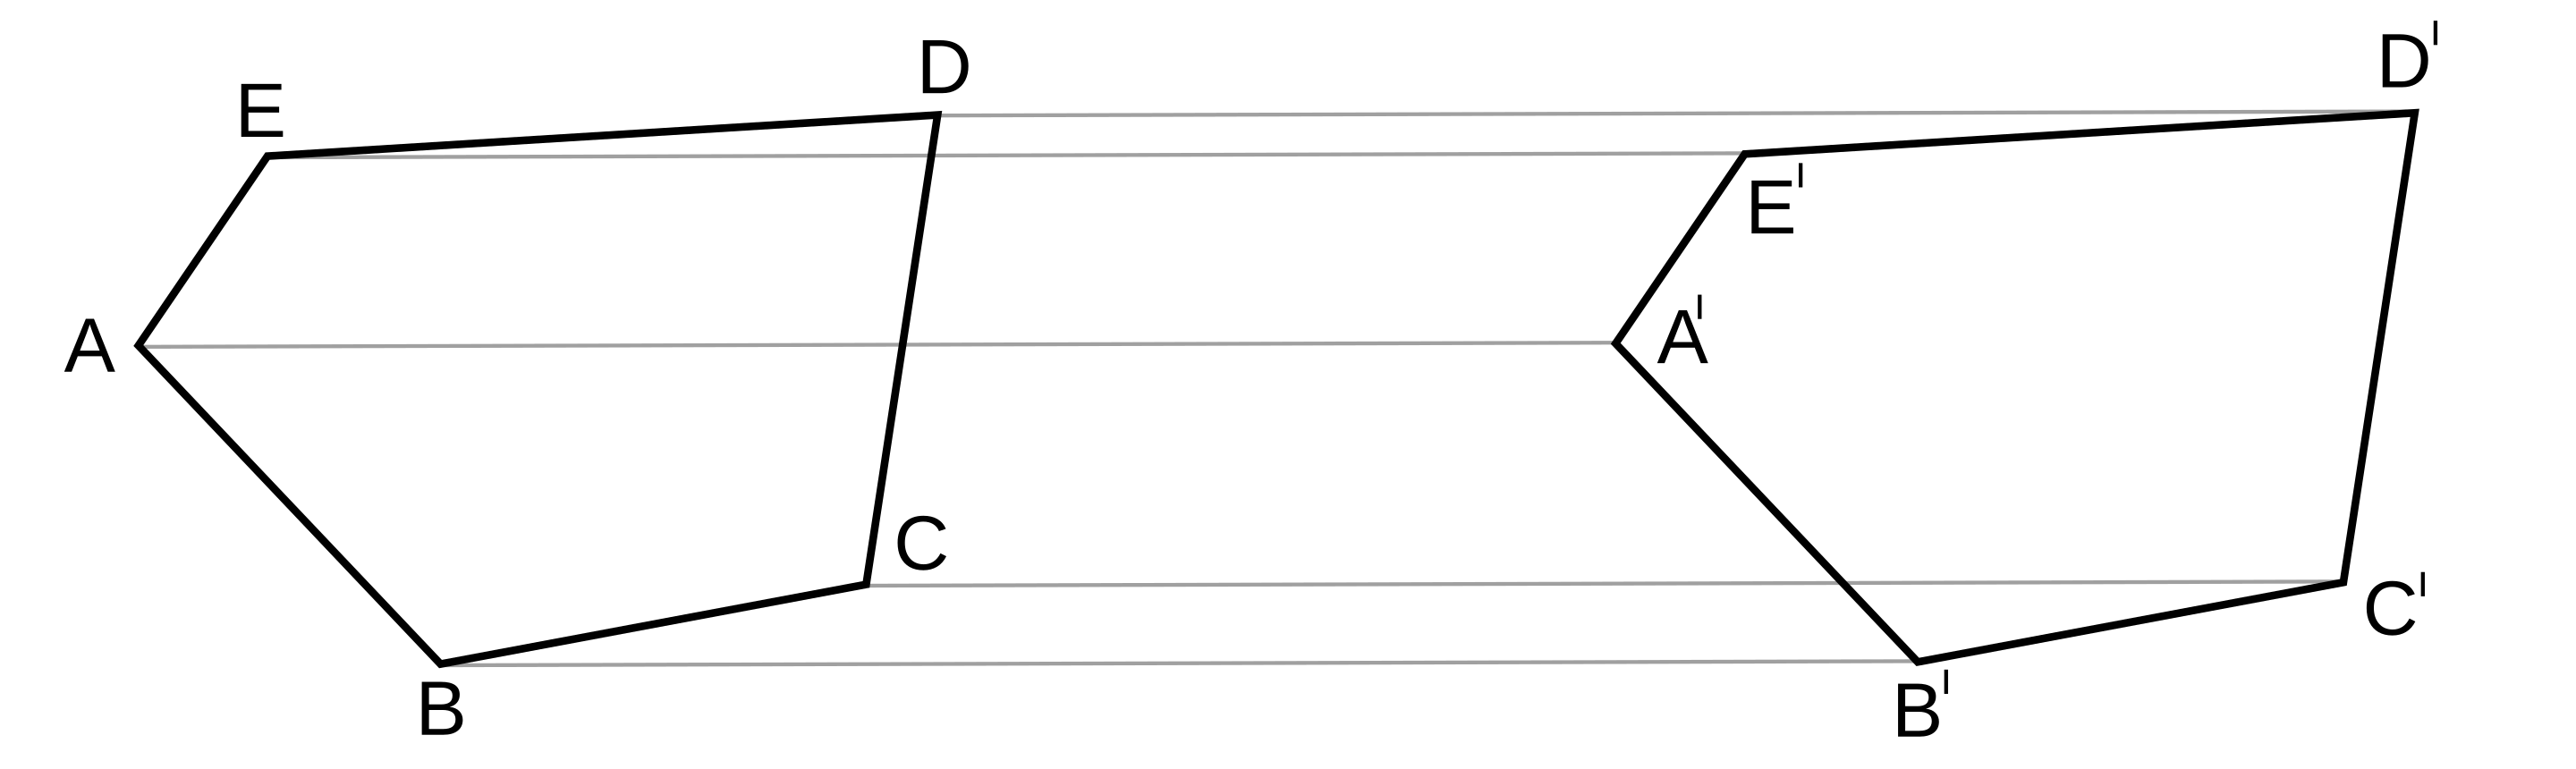
\includegraphics[width=0.5\linewidth]{img/19_posunuti.png}
                \caption{Posunutí pětiúhelníku} 
                \label{fig:enter-label}
            \end{figure}
            
        \subsubsection{Otočení (rotace) $O(S, \phi)$}
            Všechny body roviny jsou otočeny kolem středu otočení $S$ stejným směrem o úhel $\phi$.\\
            \begin{itemize}
                \item Bodu $S$ přiřazuje týž bod: $S'=S$ \\
                \item Každému bodu $X \neq S$ přiřazuje bod $X'$ tak, že $\left| XS \right| = \left| X'S \right|$ a orientovaný úhel $\measuredangle XSX'$ má velikost $\phi$.\\
            \end{itemize}
            Střed $S$ je samodružný bod.\\
            Pro $\phi = 180^{\circ}+k \cdot 360^{\circ};k \in \mathbb{Z} $ (liché násobky $180^{\circ}$), se jedná o středovou souměrnost.\\
            Pro $\phi = k \cdot 360^{\circ};k \in \mathbb{Z} $ (násobky $360^{\circ}$), se jedná o identitu.

            \begin{figure}[H]
                \centering
                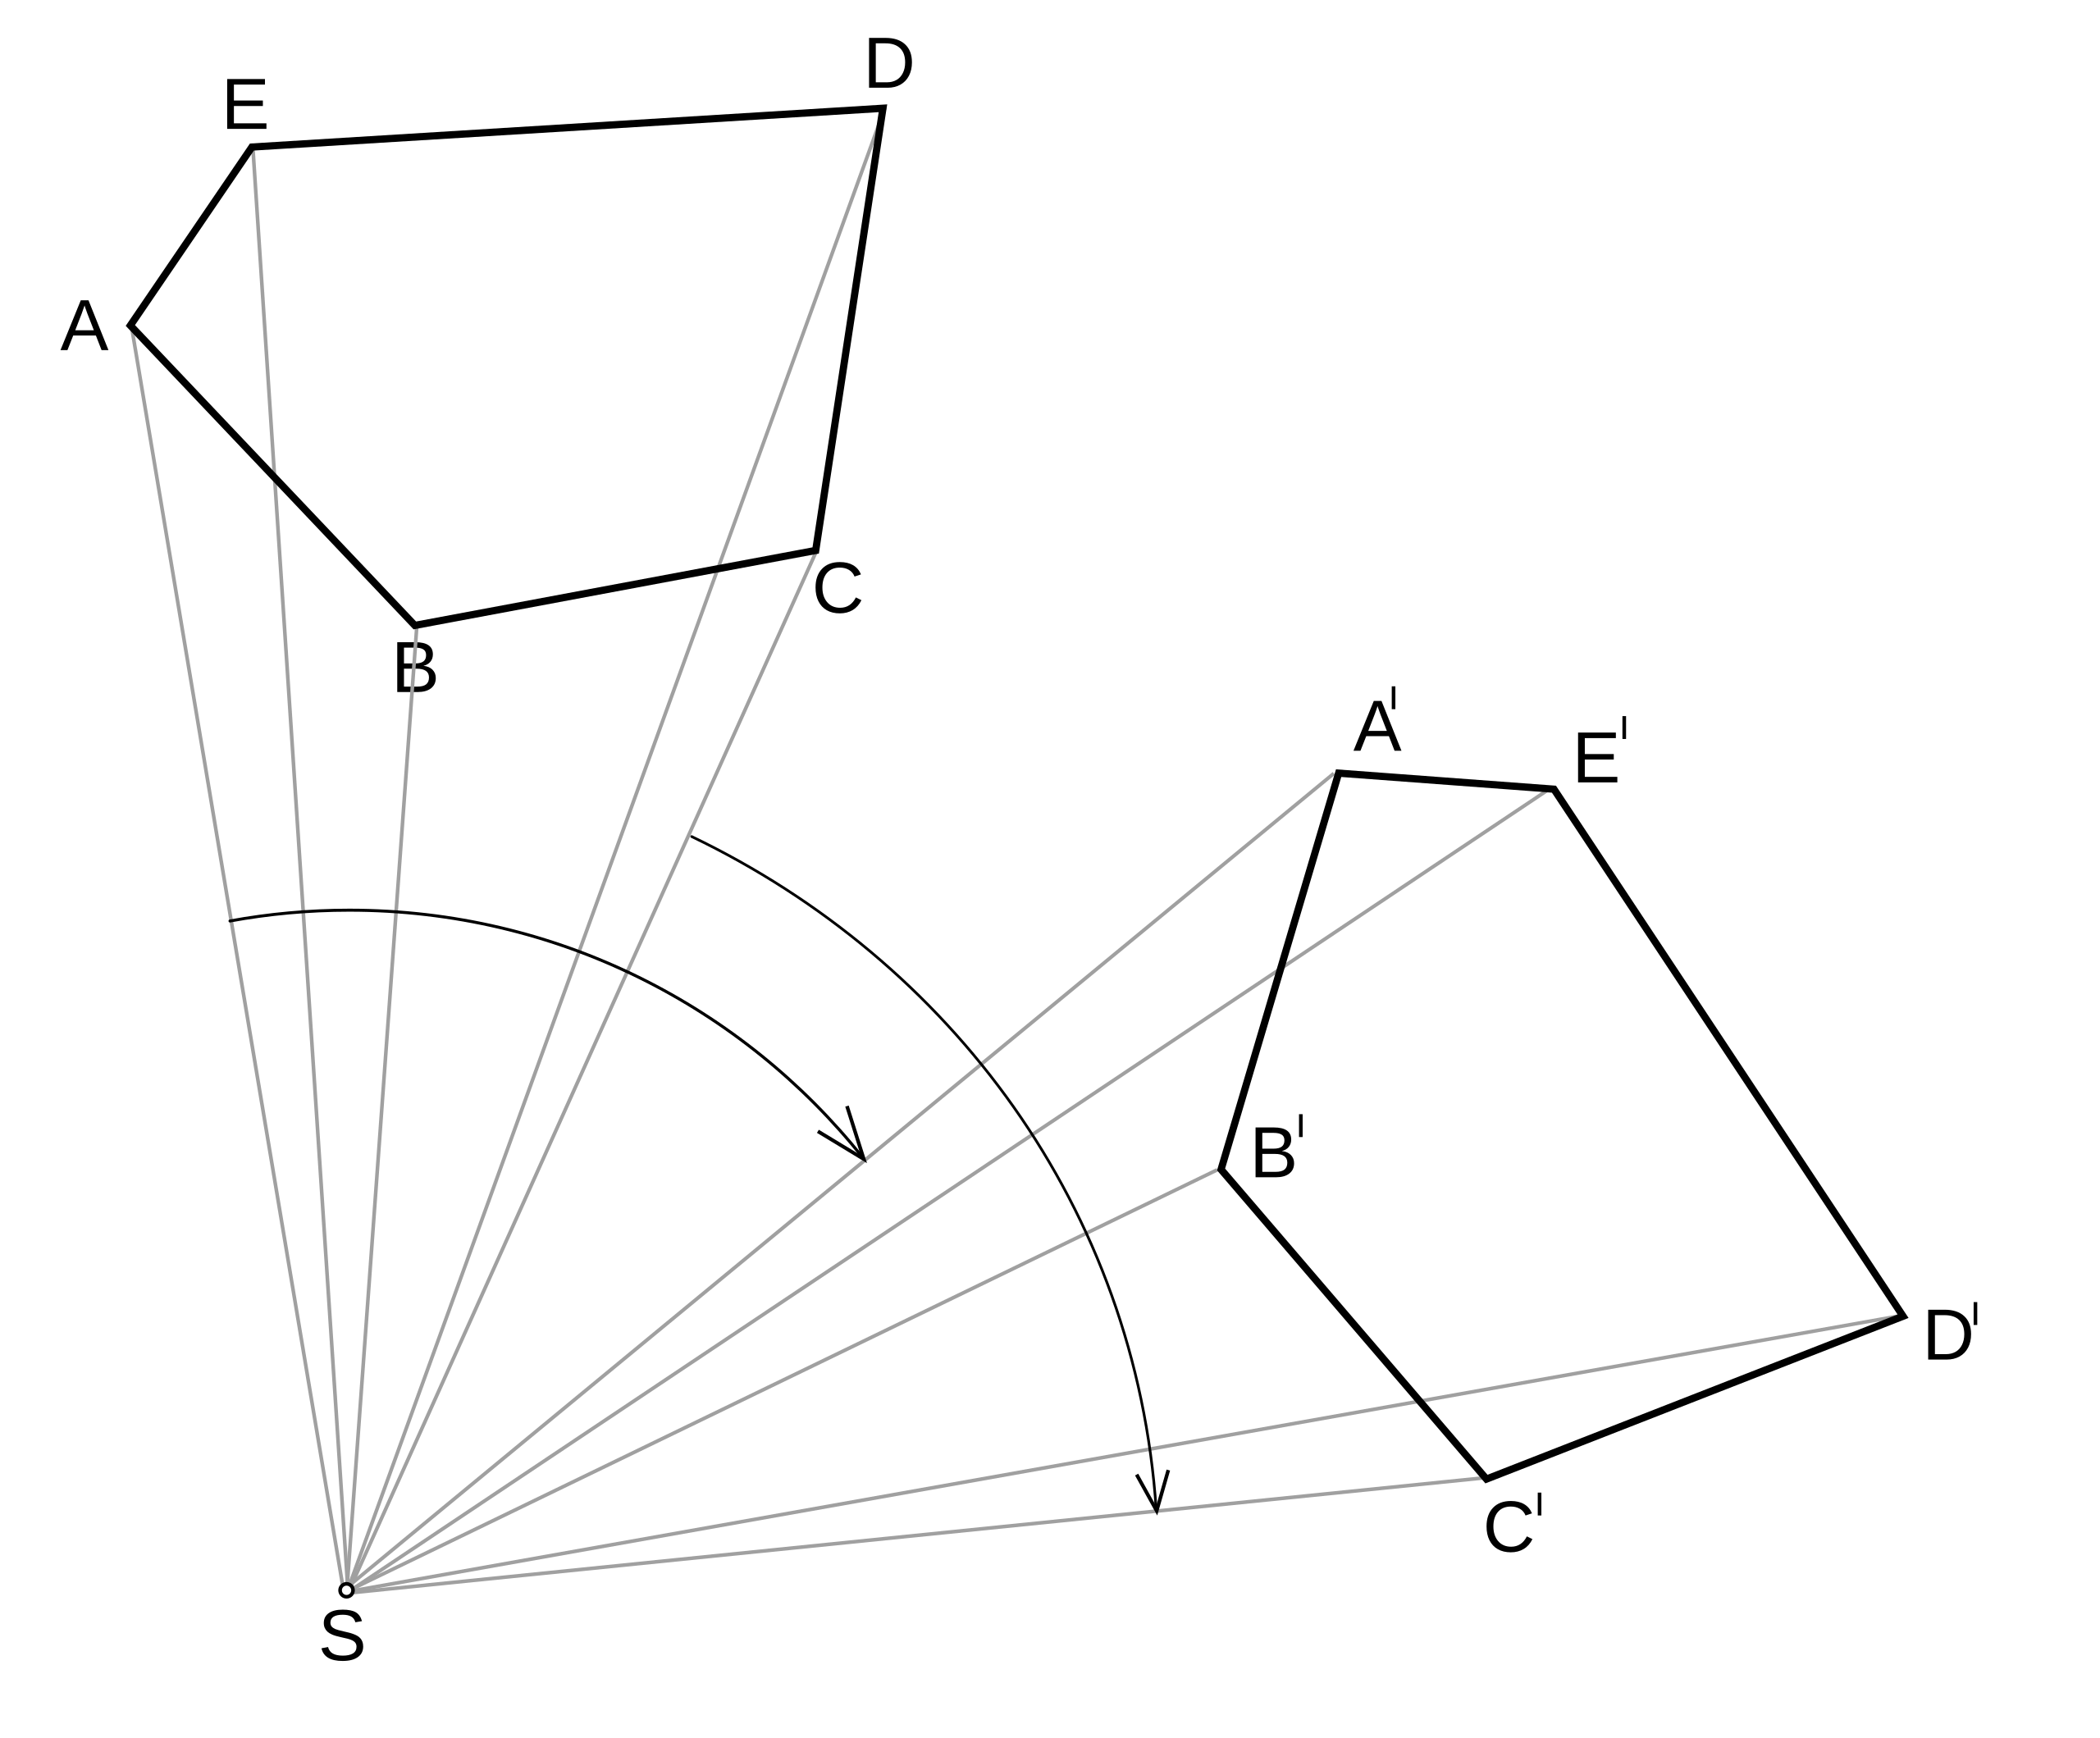
\includegraphics[width=0.5\linewidth]{img/19_otoceni.png}
                \caption{Otočení pětiúhelníku} 
                \label{fig:enter-label}
            \end{figure}
            
        \subsubsection{Středová souměrnost $S(S)$}
            Středová souměrnost je zvláštní případ otočení - otočení kolem středu o $180^{\circ}$.\\
            \begin{itemize}
                \item Středu souměrnosti $S$ přiřazuje týž bod: $S'=S$\\
                \item Bodu $X \neq S$ přiřazuje bod $X'$, který leží na polopřímce opačné k polopřímce $\mapsto SX$. Úsečka $XX'$ je bodem $S$ půlena.\\
            \end{itemize}
            Platí: $X' \in \; \mapsto XS \;\;\; \cap \;\;\; \left| XS \right| = \left| X'S \right| \;\;\; \cap \;\;\; X \neq X'$\\
            Střed $S$ je samodružný bod.

            \begin{figure}[H]
                \centering
                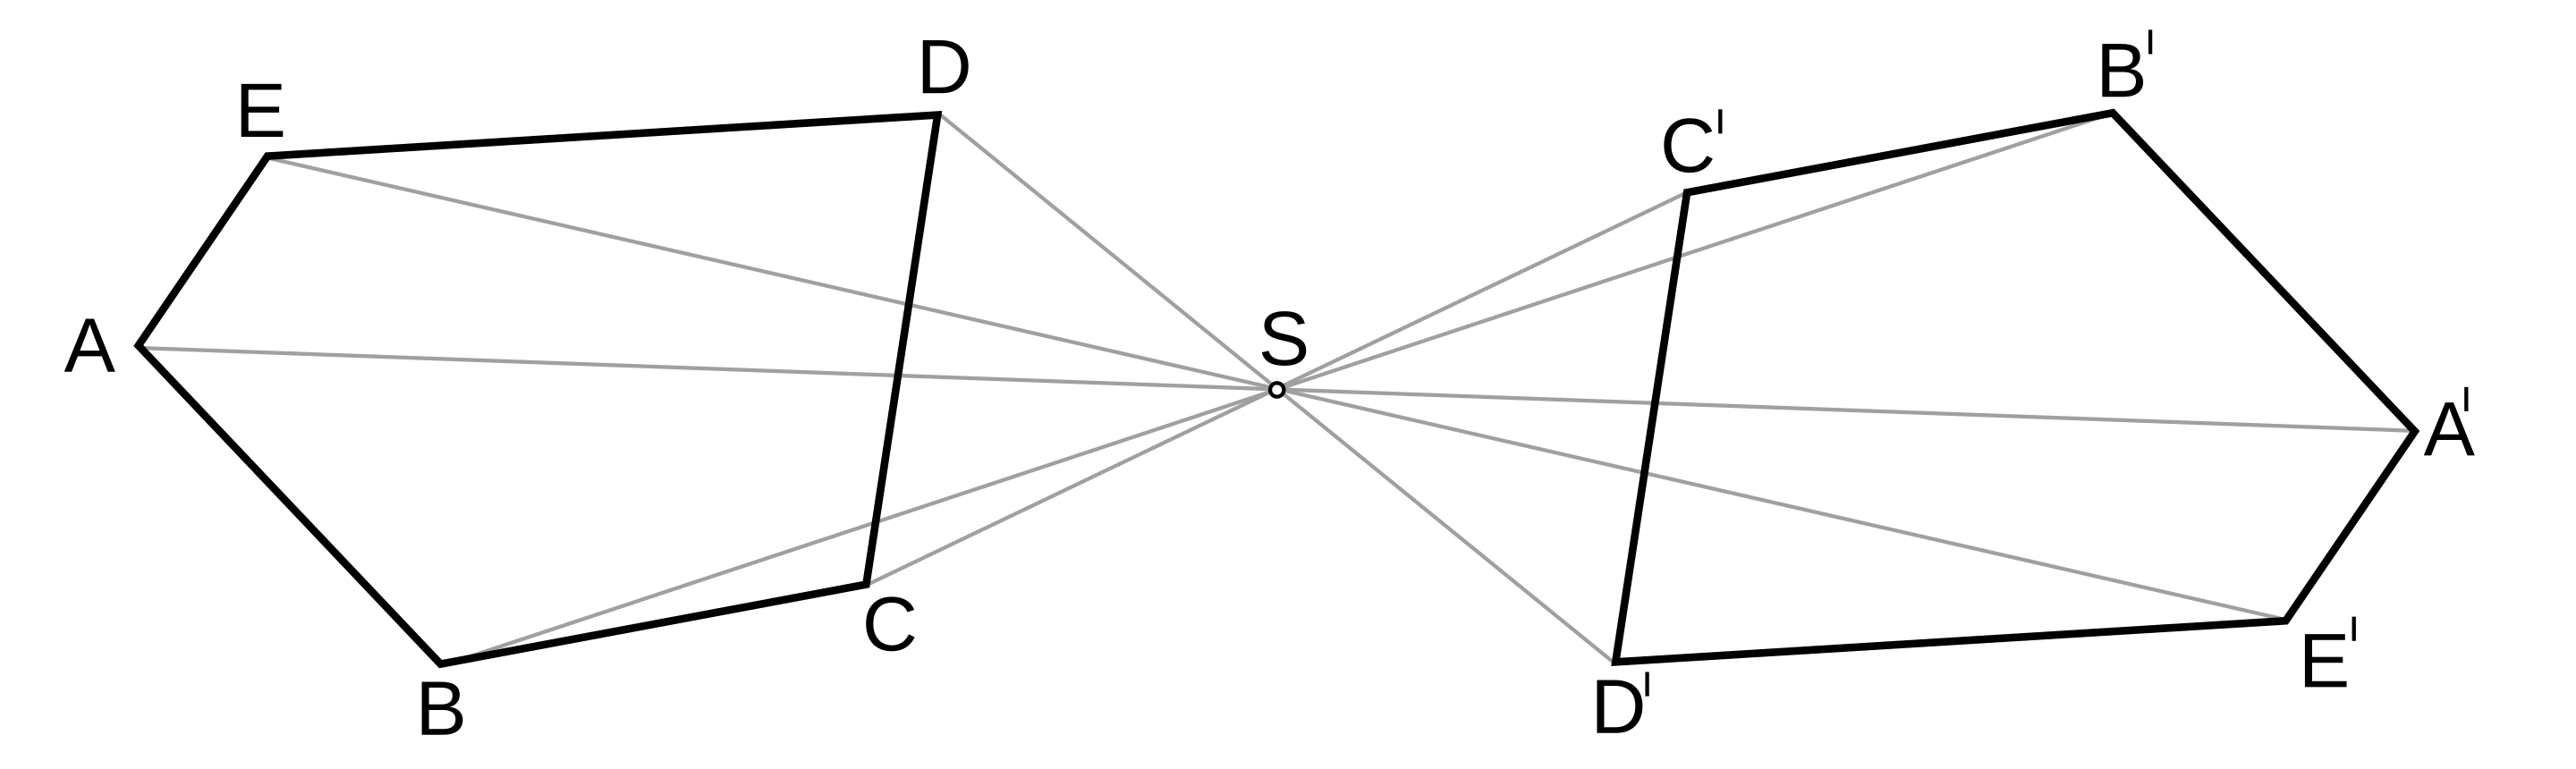
\includegraphics[width=0.5\linewidth]{img/19_stredova_soumernost.png}
                \caption{Zobrazení pětiúhelníku v středové souměrnosti} 
                \label{fig:enter-label}
            \end{figure}
            
        \subsubsection{Osová souměrnost(zrcadlení) $O(o)$}
            Osová souměrnost je shodné zobrazení, které je dané přímkou $o$ a zobrazovacím předpisem:\\
            \begin{itemize}
                \item Každému bodu $X \in o$ přiřazuje týž bod: $X'=X$
                \item Každému bodu $X \notin o$ přiřazuje bod $X'$, který leží na kolmici vedené bodem $X$ k ose $o$ tak, že úsečka $\leftrightarrow XX'$ je osou o půlena.
            \end{itemize}
            Platí: $X' \in \; \mapsto XS \;\;\; \cap \;\;\; \left| Xo \right| = \left| X'o \right| \;\;\; \cap \;\;\; X \neq X'$\\
            Všechny body osy $o$ jsou samodružné body - osa $o$ je samodružná přímka.\\
            Všechny přímky kolmé na osu $o$ jsou samodružné.

            \begin{figure}[H]
                \centering
                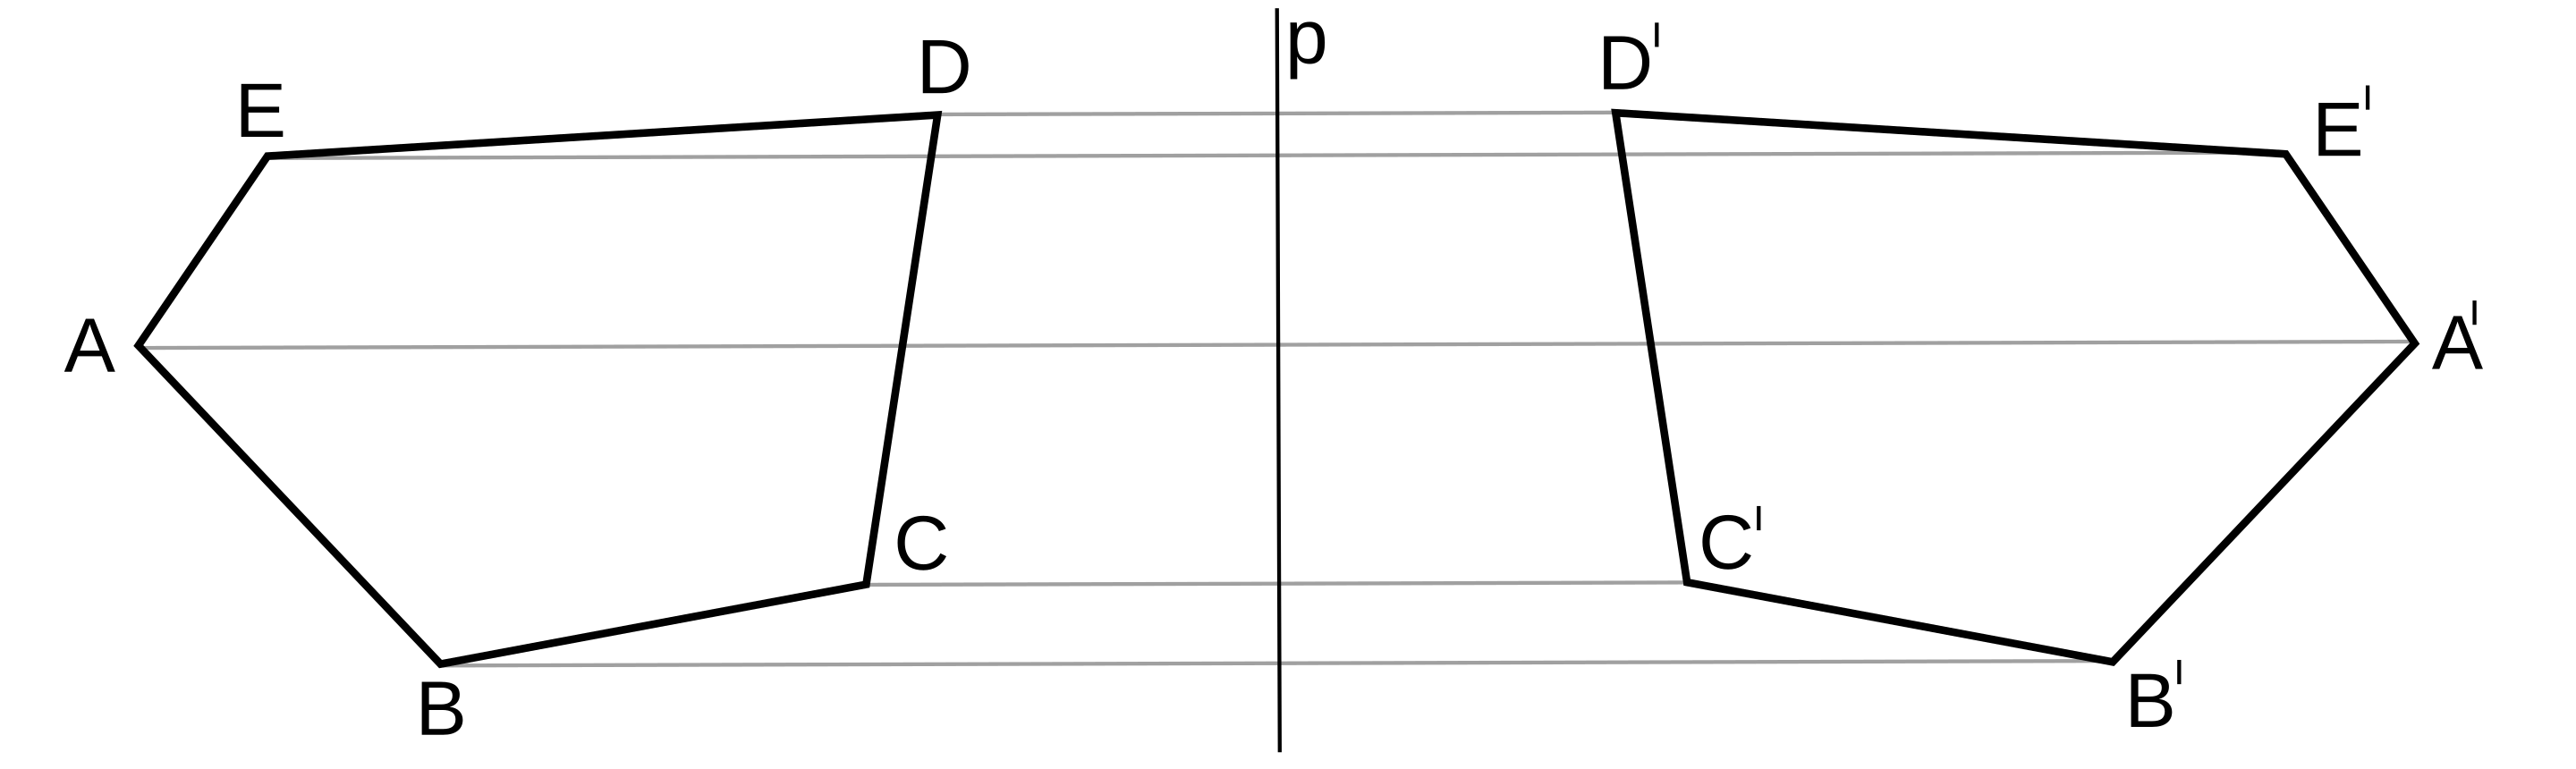
\includegraphics[width=0.5\linewidth]{img/19_osova_soumernost.png}
                \caption{Zobrazení pětiúhelníku v osové souměrnosti} 
                \label{fig:enter-label}
            \end{figure}
            
        \subsubsection{Totožnost (identita) $I()$}
            Zobrazení, které každý bod zobrazuje na sebe sama. Lze ji považovat za posunutí o úsečku nulové délky nebo za otočení o nulový úhel.\\
            Každý bod je samodružný.

            \begin{figure}[H]
                \centering
                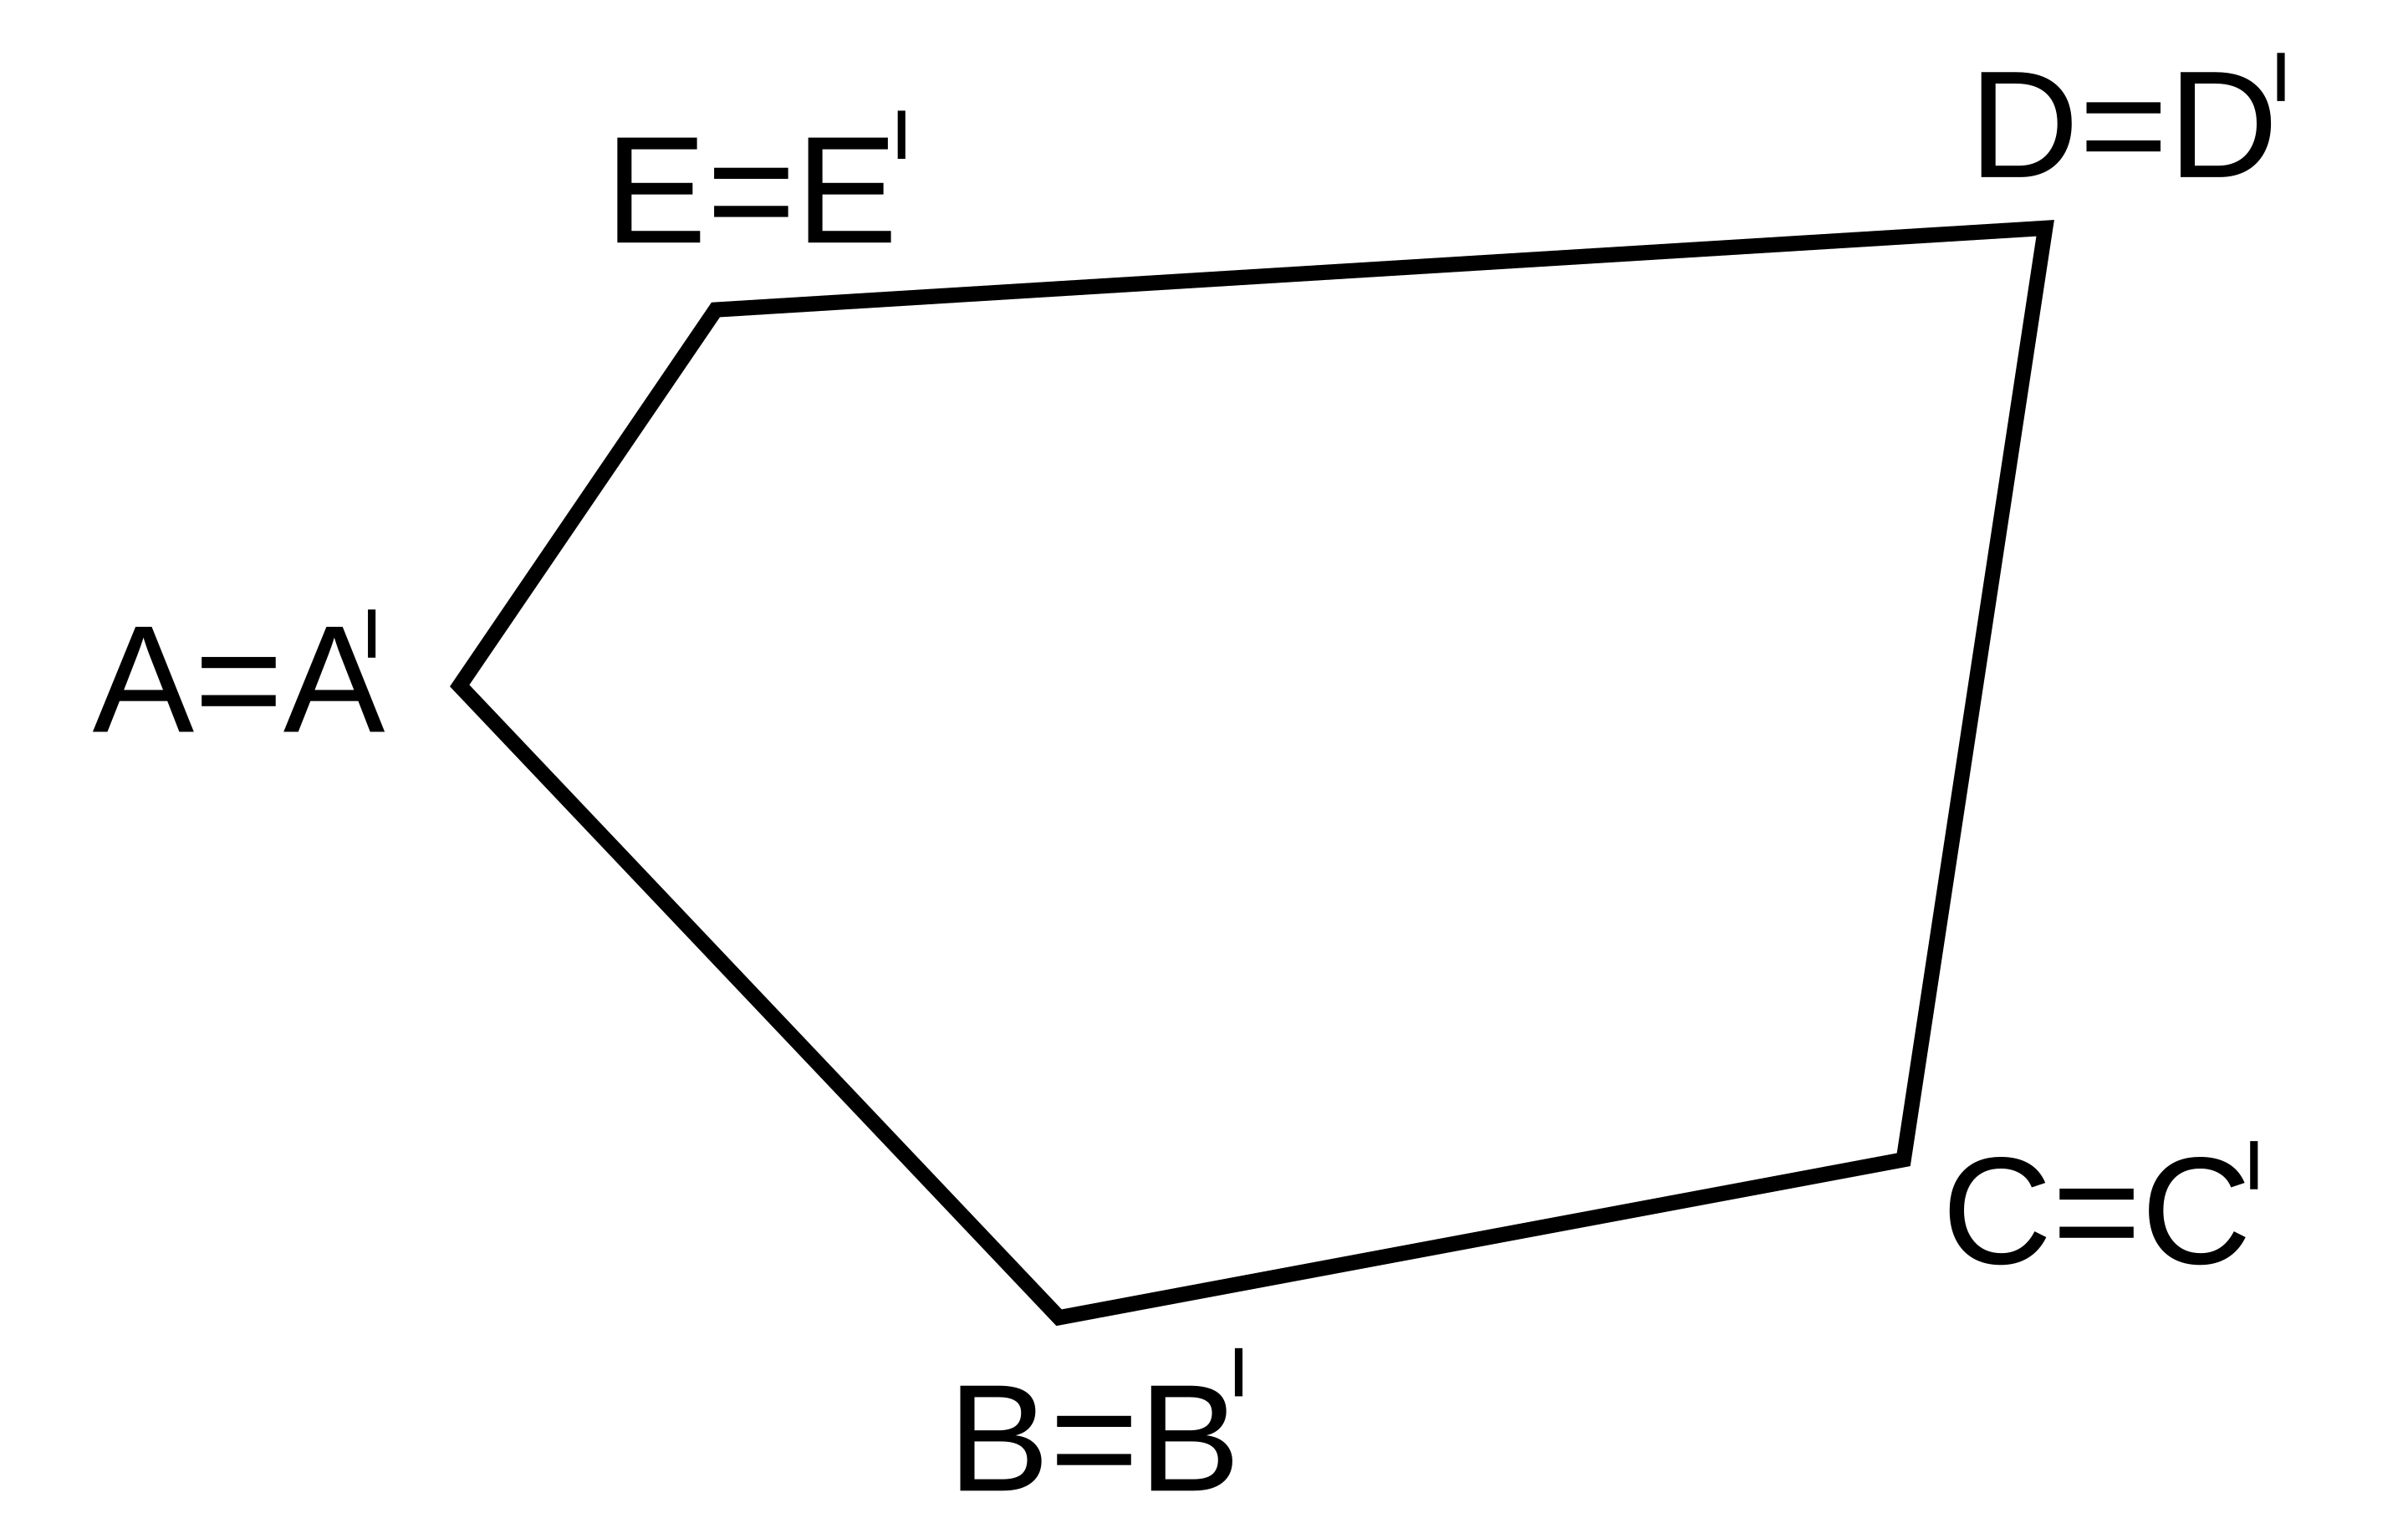
\includegraphics[width=0.5\linewidth]{img/19_identita.png}
                \caption{Geometrická identita} 
                \label{fig:enter-label}
            \end{figure}
            
    \subsection{Skládání shodných zobrazení}
        Shodné zobrazení shodného zobrazení je jen dalsí shodné zobrazení.
        \begin{itemize}
            \item Složením dvou posunutí je opět posunutí.
            \item Složením dvou středových souměrností je posunutí.
            \item Složením dvou otočení se stejným středem je opět otočení se stejným středem.
            \item Složením dvou osových souměrností se stejnou osou je identita.
            \item Složením dvou osových souměrností s různými rovnoběžnými osami je posunutí.
            \item Složením dvou osových souměrností s různoběžnými osami je otočení kolem průsečíku os, úhel $\phi$ je dvojnásobek úhlu, který osy svírají.
        \end{itemize}

    \subsection{Přímá a nepřímá shodnost}
        Vrcholy vzorového trojúhelníku jsou pojmenovány proti směru hodinových ručiček.\\
        Po posunutí, otočení, středové souměrnosti si trojúhelník \textbf{zachová orientaci}. Trojúhleník je \textbf{přímo shodný}.\\
        Naopak po osové souměrnosti se pořadí vrcholů otočí. Osová souměrnost \textbf{mění orientaci}. Trojúhleník je \textbf{nepřímo shodný}.\\
        Shodnost zachovávající orientaci se nazývá přímá neboli přemístění. Shodnost měnící orientaci se nazývá nepřímá.\\
        \begin{itemize}
            \item Složením přímých shodností je přímá shodnost.
            \item Složením sudého počtu nepřímých shodností je přímá shodnost.
            \item Složením lichého počtu nepřímých shodností je nepřímá shodnost.
        \end{itemize}
\title{ 15. Kuželosečky - kružnice, elipsa}
\author{Aneta Foralová}
\date{30.4.2025}

\maketitle

\section{Kružnice, elipsa}


\begin{figure}[H]
        \centering
        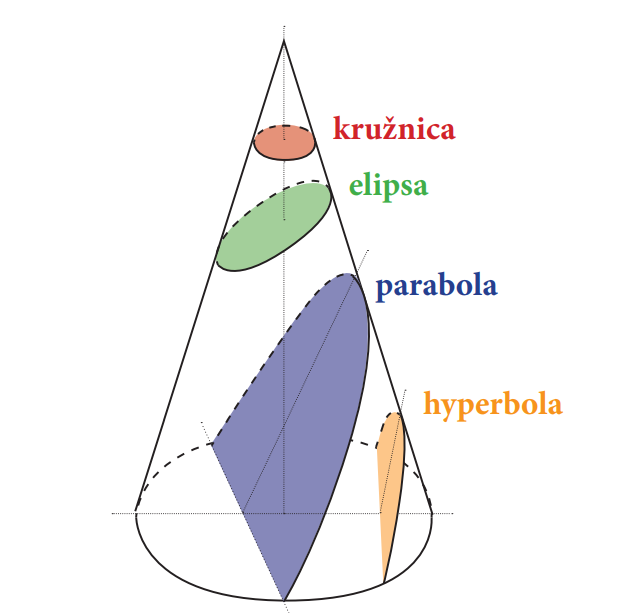
\includegraphics[width=0.3\linewidth]{img/14_kuzelosecky.png}
        \caption{Kuželosečky} 
        \label{fig:enter-label}
    \end{figure}    

\subsection{Definice}
    Pojem \textbf{KUŽELOSEČKY} vznikl jako název množin bodů v prostoru, které lze získat jako průniky roviny a kuželové plochy.\\
    
    Nechť je dán v rovině $E_2$ bod $S$ a číslo $r \in \mathbb{R}$, $r > 0$. \textbf{KRUŽNICE} je množina všech bodů v rovině, které leží ve stejné vzdálenosti, označované jako poloměr, od pevně daného bodu, zvaného střed.\\
    
    Nechť jsou dány v rovině $E_2$ dva různé body $F$ a $G$. \textbf{ELIPSA} je množina všech bodů v rovině, které mají stálý součet vzdáleností ($2a$) od dvou pevně daných bodů, tzv. ohnisek.\\

    Je-li střed elipsy bod $S[0;0]$ poté platí:\\
    Číslo  $e > 0$ se nazývá \textbf{excentricita elipsy} a platí: $e^2 = a^2 - b^2 , a > b$\\
    Body $A[a;0], B[-a;0]$ se nazývají \textbf{hlavní vrcholy elipsy}\\ $a>0$ se nazývá \textbf{hlavní poloosa elipsy}\\ Body $C[0;b], D[0;-b]$ se nazývají \textbf{vedlejší vrcholy elipsy}\\$b>0$ se nazývá \textbf{vedlejší poloosa elipsy}\\
    

    \begin{figure}[H]
        \centering
        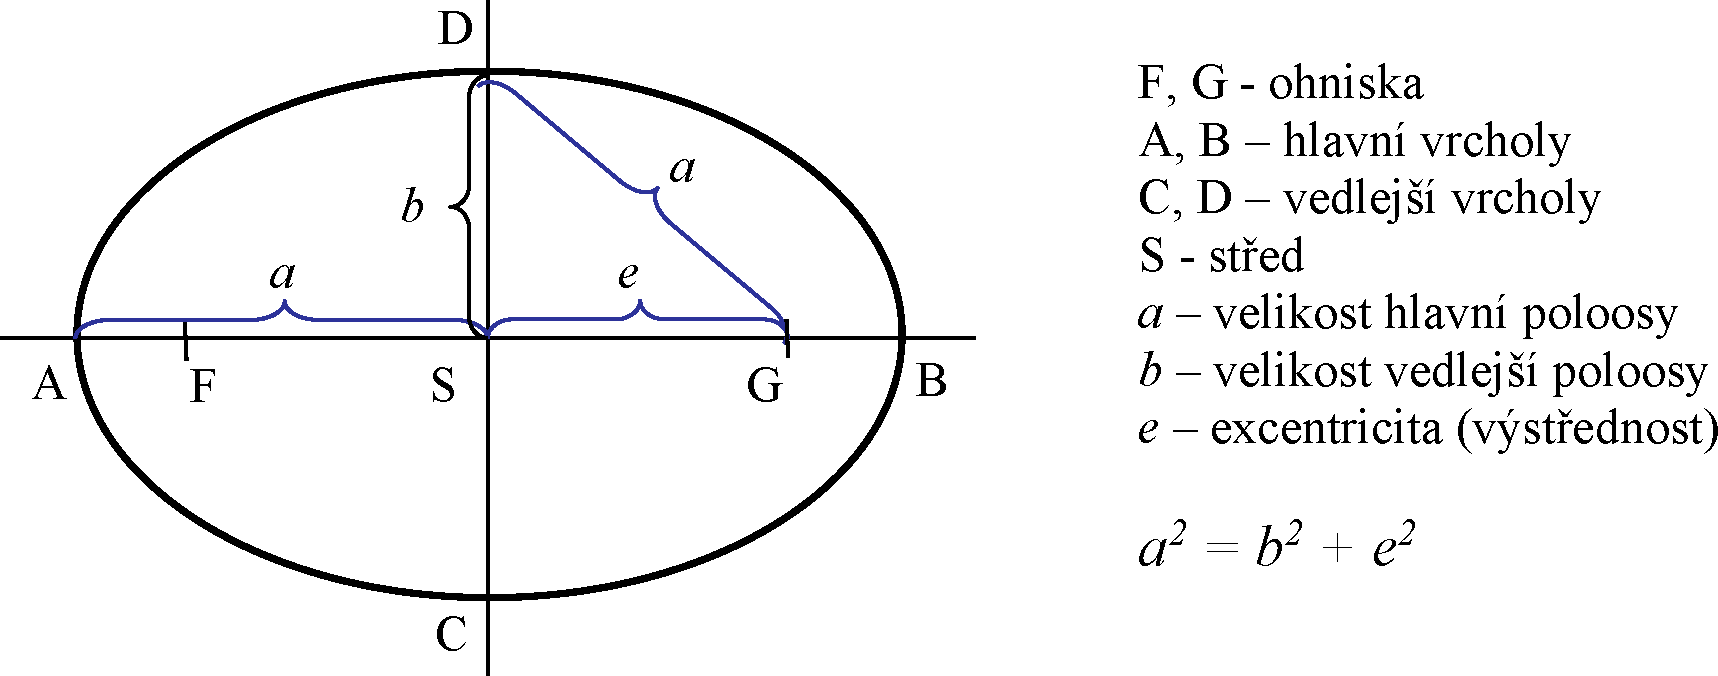
\includegraphics[width=0.6\linewidth]{img/14_elipsa1.png}
        \caption{Elipsa} 
        \label{fig:enter-label}
    \end{figure}    

\subsection {Středové a obecné rovnice}
    Obecnou rovnici kuželosečky získáme ze středové rovnice provedením operací ve středové rovnici a zavedením nových konstant\\
    Středovou rovnici kuželosečky získáme z obecné rovnice doplněním na čtverec
\subsubsection{Kružnice}
    Je-li S[0;0] středová rovnice kružnice je: 
    $$
    x^2 + y^2 = r^2
    $$
    A je-li S[$m;n$] a $r>0$, je středová rovnice kružnice 
    $$
    (x-m)^2 + (y-n)^2 = r^2
    $$
    Obecná rce kružnice je 
    $$
    x^2 + y^2 - 2mx - 2ny+q=0,
    $$
    kde $p=m^2 + n^2-r^2$\\
    \vspace{1em} 
    
    \begin{figure}[H]
        \centering
        \includegraphics[width=0.3\linewidth]{img/14_kružnice.png}
        \caption{Kružnice} 
        \label{fig:enter-label}
    \end{figure}

\subsubsection{Elipsa}
    Jeli S[0;0] a elipsa je umístěna horizontálně tedy A[$a$;0] a B[$-a$;0] pak středová rovnice elipsy je  
    $$
    \frac{x^2}{a^2} + \frac{y^2}{b^2}=1
    $$\\ 
    \vspace{1em}
    
    \begin{figure}[H]
        \centering
        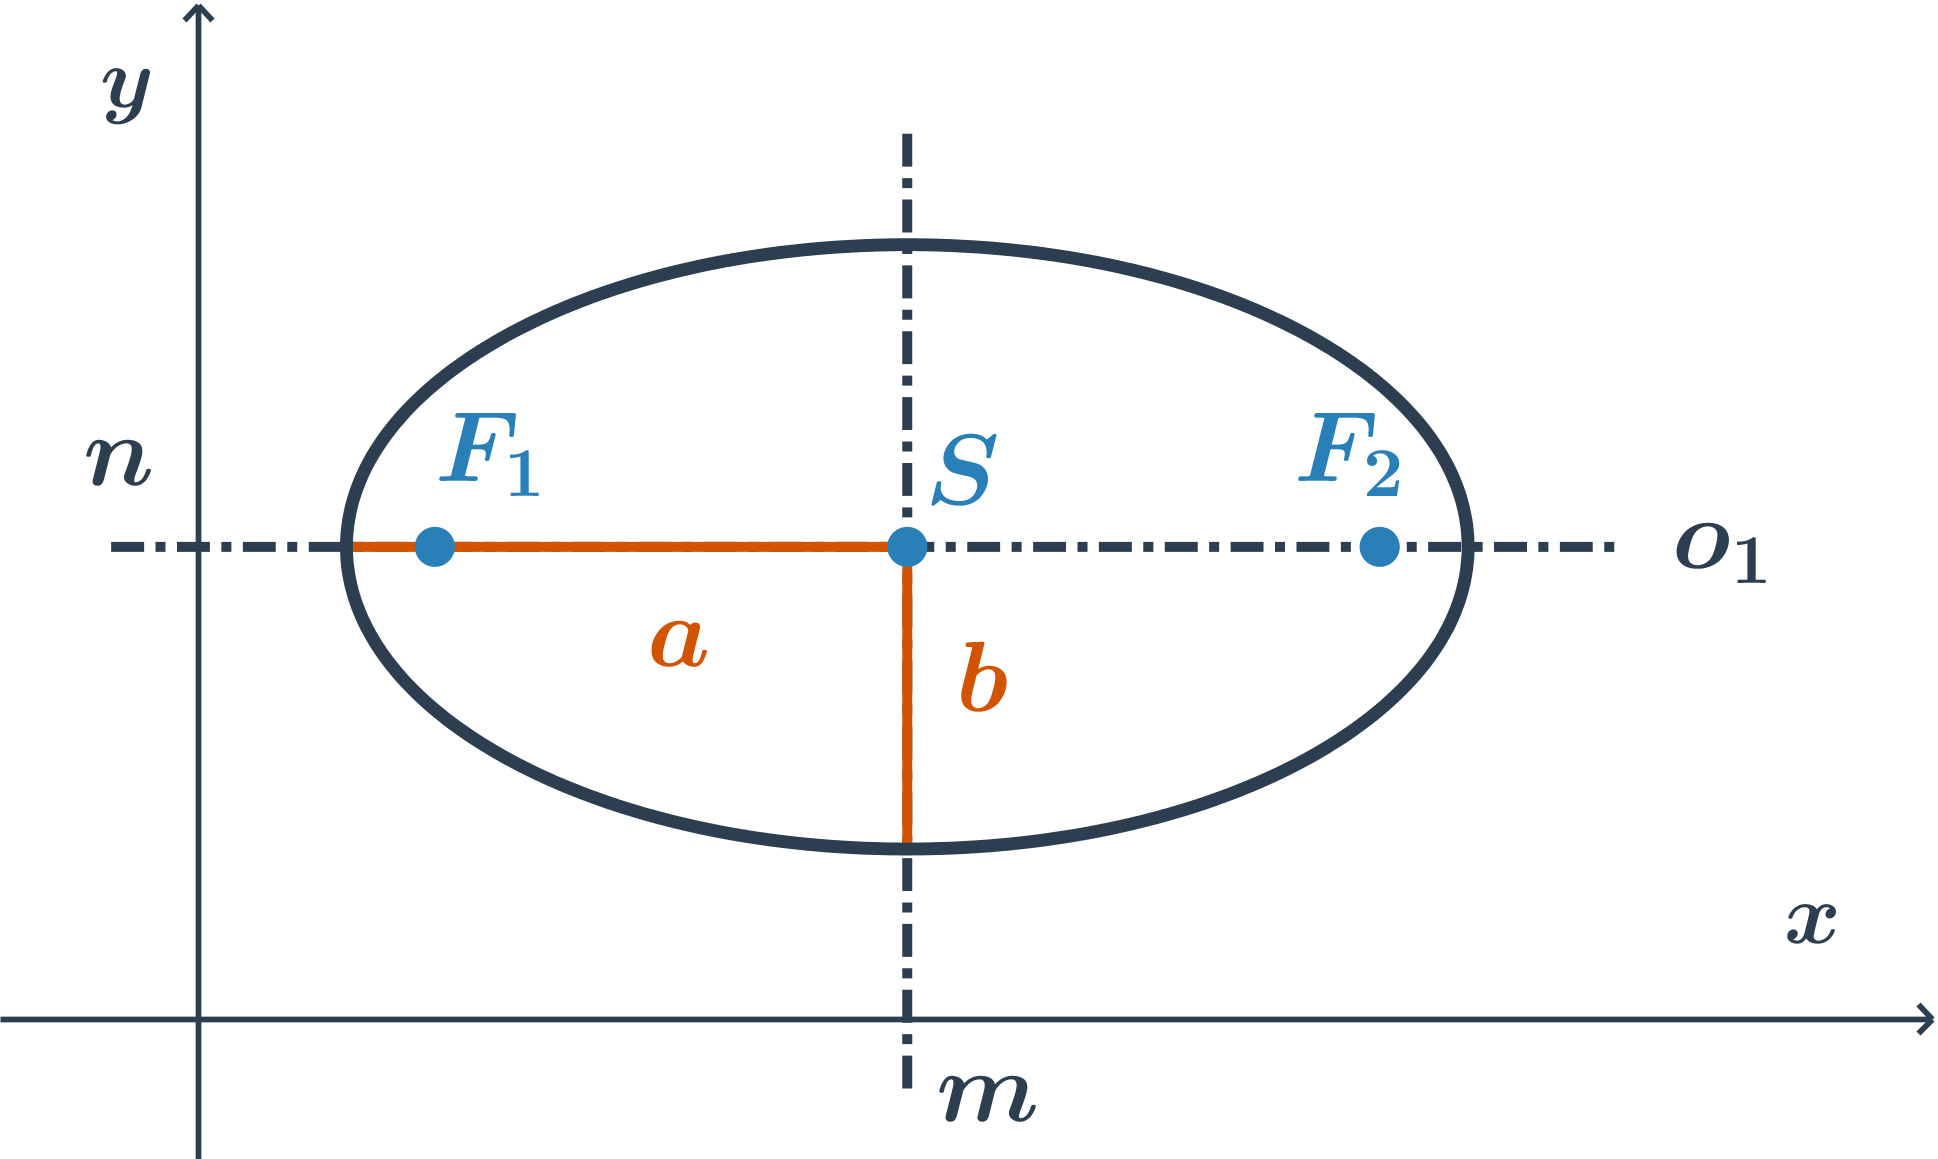
\includegraphics[width=0.5\linewidth]{img/14_elipsa3.png}
        \caption{Elipsa s hlavní poloosou x} 
        \label{fig:enter-label}
    \end{figure}
    
  
    \vspace{1em}
    Jeli S[0;0] a elipsa je umístěna vertikálně tedy A[0;$a$] a D[$b$;0], $a > b$ pak středová rovnice elipsy je  
    $$
    \frac{x^2}{b^2} + \frac{y^2}{a^2}=1
    $$\\
    \vspace{1em} 
    
    \begin{figure}[H]
        \centering
        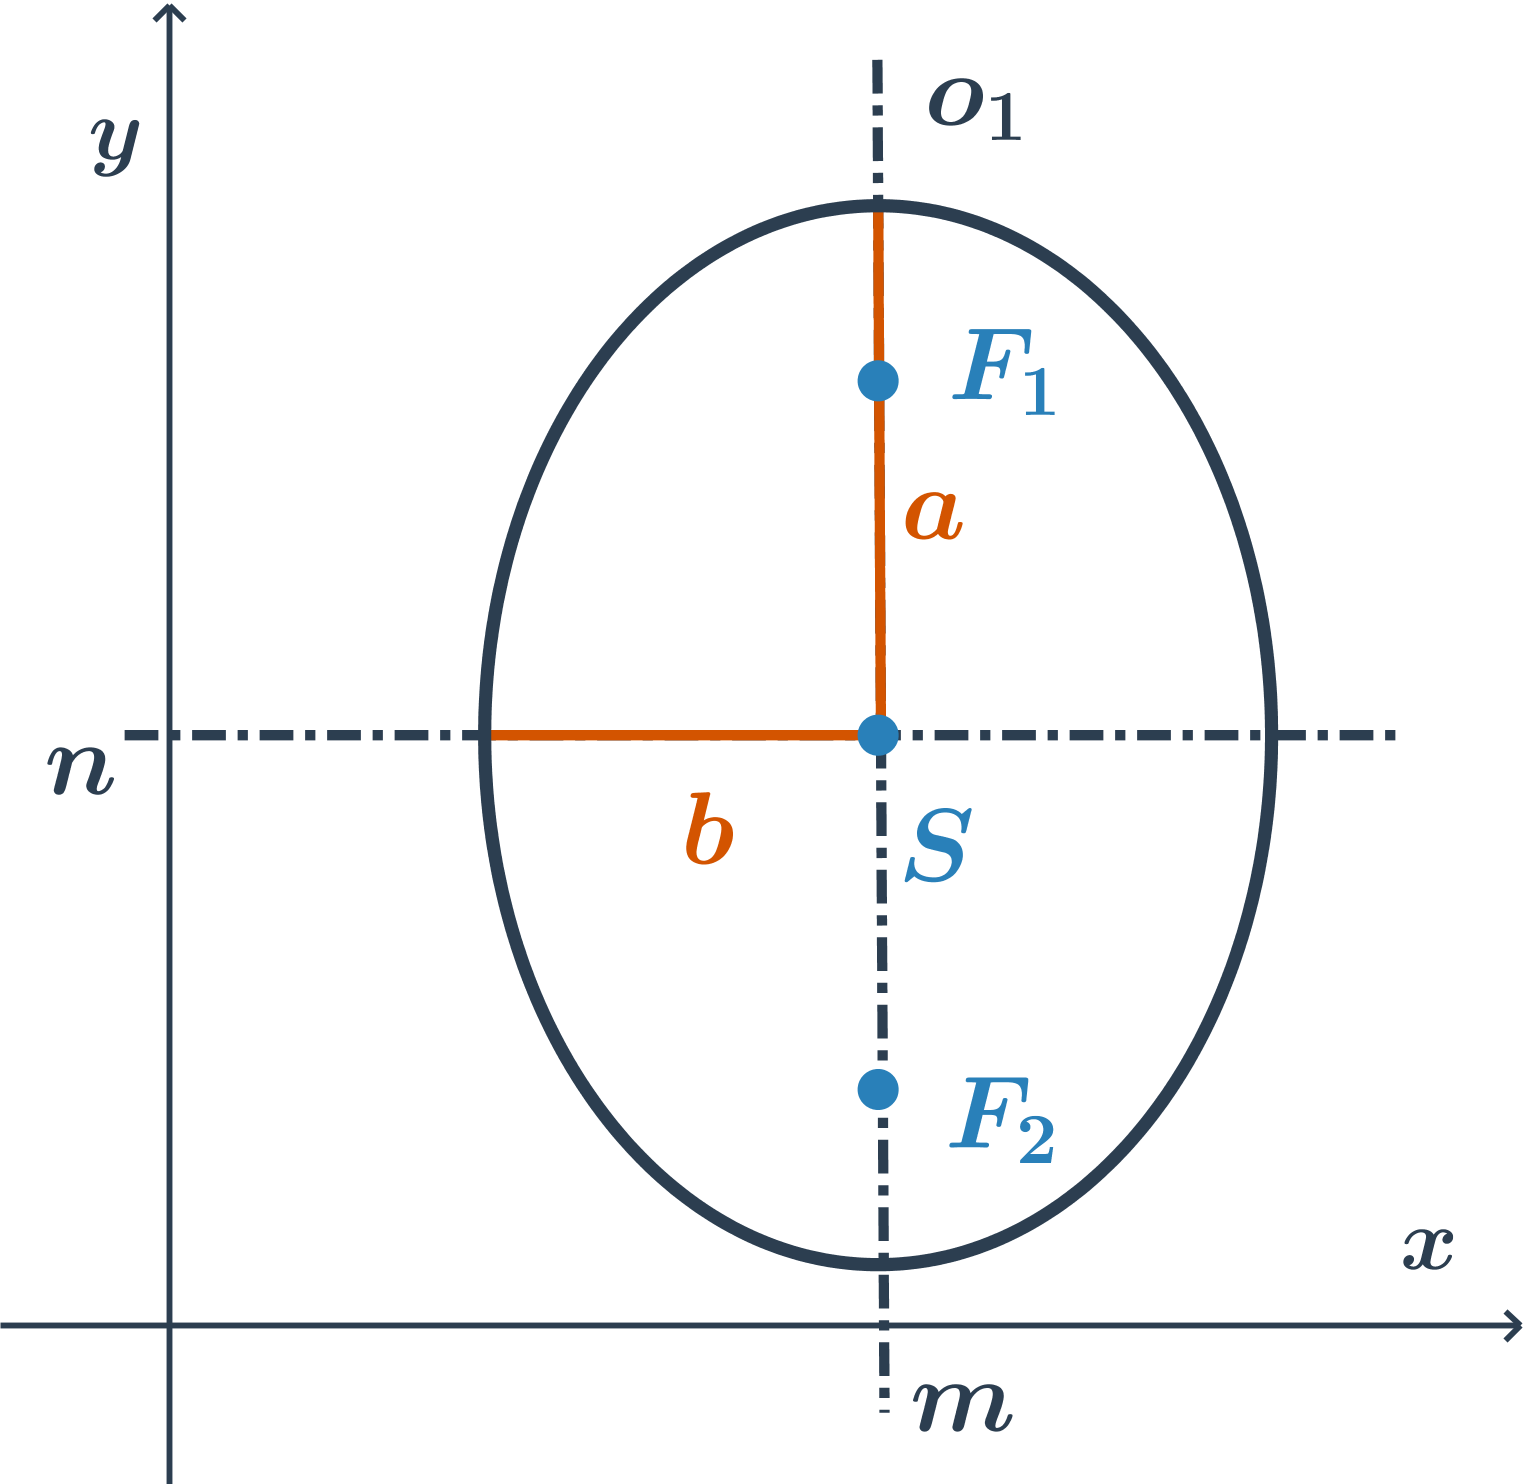
\includegraphics[width=0.3\linewidth]{img/14_elipsa 2.png}
        \caption{Elipsa s hlavní poloosou y} 
        \label{fig:enter-label}
    \end{figure}
    
    \vspace{1em}
    Je-li $S[m;n], a>0 $ , $ b>0 $ , $ a>b$ je středová rovnice elipsy: 
    $$
    \frac{(x-m)^2}{a^2} + \frac{(y-n)^2}{b^2}=1
    $$ 
    Obecná rce elipsy je: $px^2+qy^2+2rx+2sy+t=0$, kde $pq>0$
\subsection{Vzájemná poloha kuželosečky a bodu}
    Nechť je dána obecná rovnice kuželosečky a bod $A[x_A,y_A]$. Označíme si levou stranu obecné rovnice kuželosečky $f(x,y)$ pro každý bod kuželosečky a dosadíme souřadnice bodu $A[x_A,y_A]$ a pro jednotlivé kuželosečky platí: \begin{itemize}
        \item $A$ je bodem kuželosečky právě tehdy když $f(x_A,y_a)=0$
        \item $A$ je vnějším bodem kuželosečky právě když $f(x_A,y_a)>0$
        \item $A$ je vnitřním bodem kuželosečky právě když $f(x_A,y_a)<0$
    \end{itemize}
\subsection{Vzájemná poloha kuželosečky a přímky}
    Vzájemnou polohu kuželosečky a přímky určujeme tak, že hledáme jejich společné body. Analyticky to znamená, že hledáme řešení soustavy lineární rce (přímka) a kvadratické rce (kuželosečka) o dvou neznámých. To nakonec vede k řešení kvadratické rce o jendé neznáme. Ta může mít: \begin{itemize}
        \item Pro $D>0$ - dva společné body tj. sečna
        \item Pro $D=0$ - jedno řešení tj. tečna
        \item Pro $D<0$ - žádné řešení tj. vnější přímka
    \end{itemize}
\subsection{Vzájemná poloha kuželoseček}
    Vzájemná poloha kuželoseček se zkoumá opět tak, že se hledají společné body, analyticky to znamená, že se řeší soustava dvou kvadratických rovnic o dvou neznámých

\title{ 16. Kuželosečky - parabola, hyperbola}
\author{Aneta Foralová}
\date{1.5.2025}

\maketitle

\section{Parabola, hyperbola}


\begin{figure}[H]
        \centering
        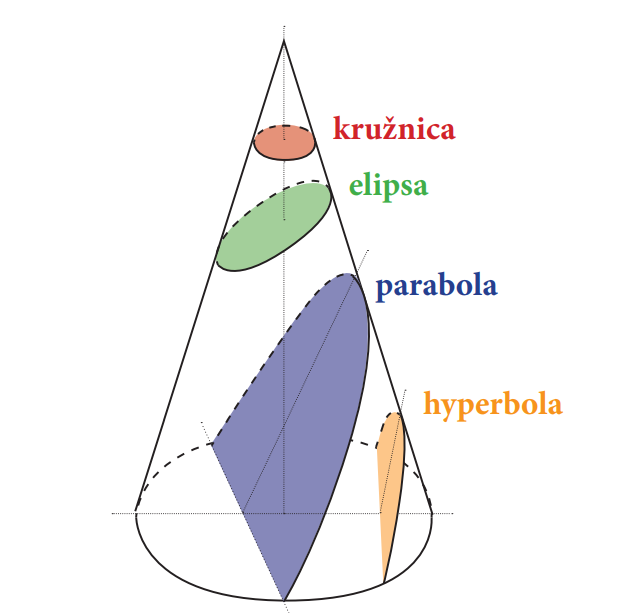
\includegraphics[width=0.3\linewidth]{img/14_kuzelosecky.png}
        \caption{Kuželosečky} 
        \label{fig:enter-label}
    \end{figure}   
    

\subsection{Definice}
    Pojem \textbf{KUŽELOSEČKY} vznikl jako název množin bodů v prostoru, které lze získat jako průniky roviny a kuželové plochy.\\
    
    Nechť je dána v rovině $E_2$ přímka $d$ a bod $F$, $F$ $\notin d$.\textbf{PARABOLA} je množina všech bodů $X$ roviny $E_2$, které mají stejnou vzdálenost od bodu $F$ i od přímky $d$\\
    
    Nechť jsou dány v rovině $E_2$ dva různé body $F$ a $G$. \textbf{HYPERBOLA} je množina všech bodů $X$ v rovině $E_2$, které mají od bodů $F$ a $G$ konstantní rozdíl vzdálenosti\\
    
    Přímka $d$ se nazývá \textbf{řídící přímka} paraboly, $V$ je \textbf{vrchol} paraboly a číslo $p$ nazýváme \textbf{parametr} a body $F$ a $G$ jsou jak u elipsy \textbf{ohniska} (U paraboly pouze 1)\\
    
    Číslo $e$ se nazývá \textbf{excentricita }hyperboly a platí $e^2=a^2 + b^2$, \textbf{Asymptoty} hyperboly jsou přímky, ke kterým se ramena hyperboly blíží, ale nikdy se jich nedotknou, určují její směr a mají tvar: $a_1: y=\frac{b/a}{a/b}x,a_2: y=-\frac{b/a}{a/b}x$
    
    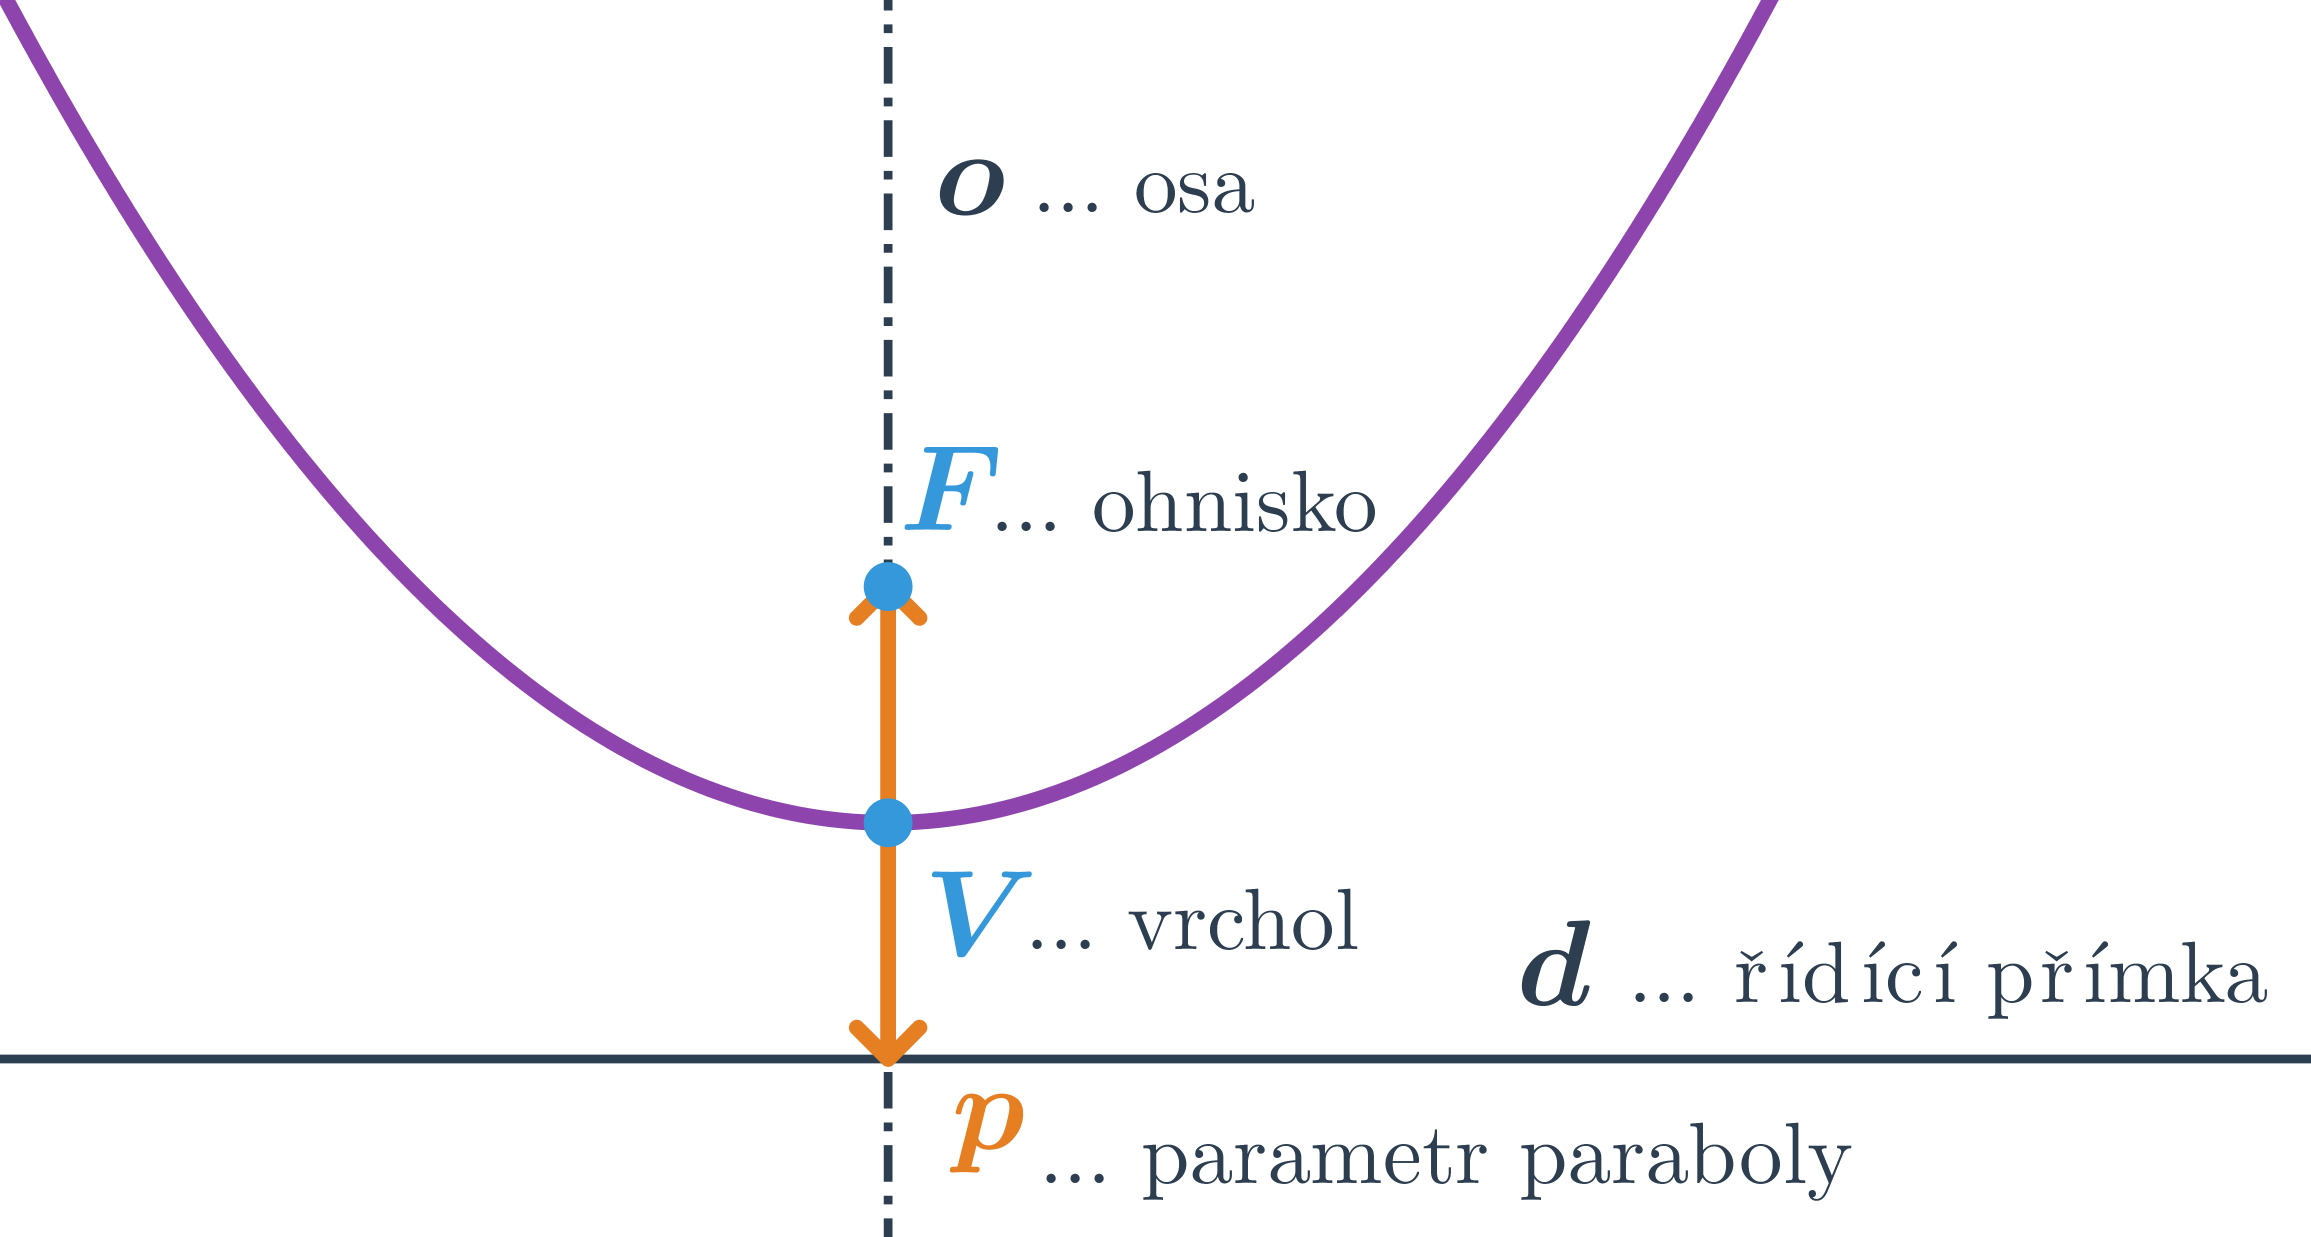
\includegraphics[width=0.45\linewidth]{img/14_parabola1.png} 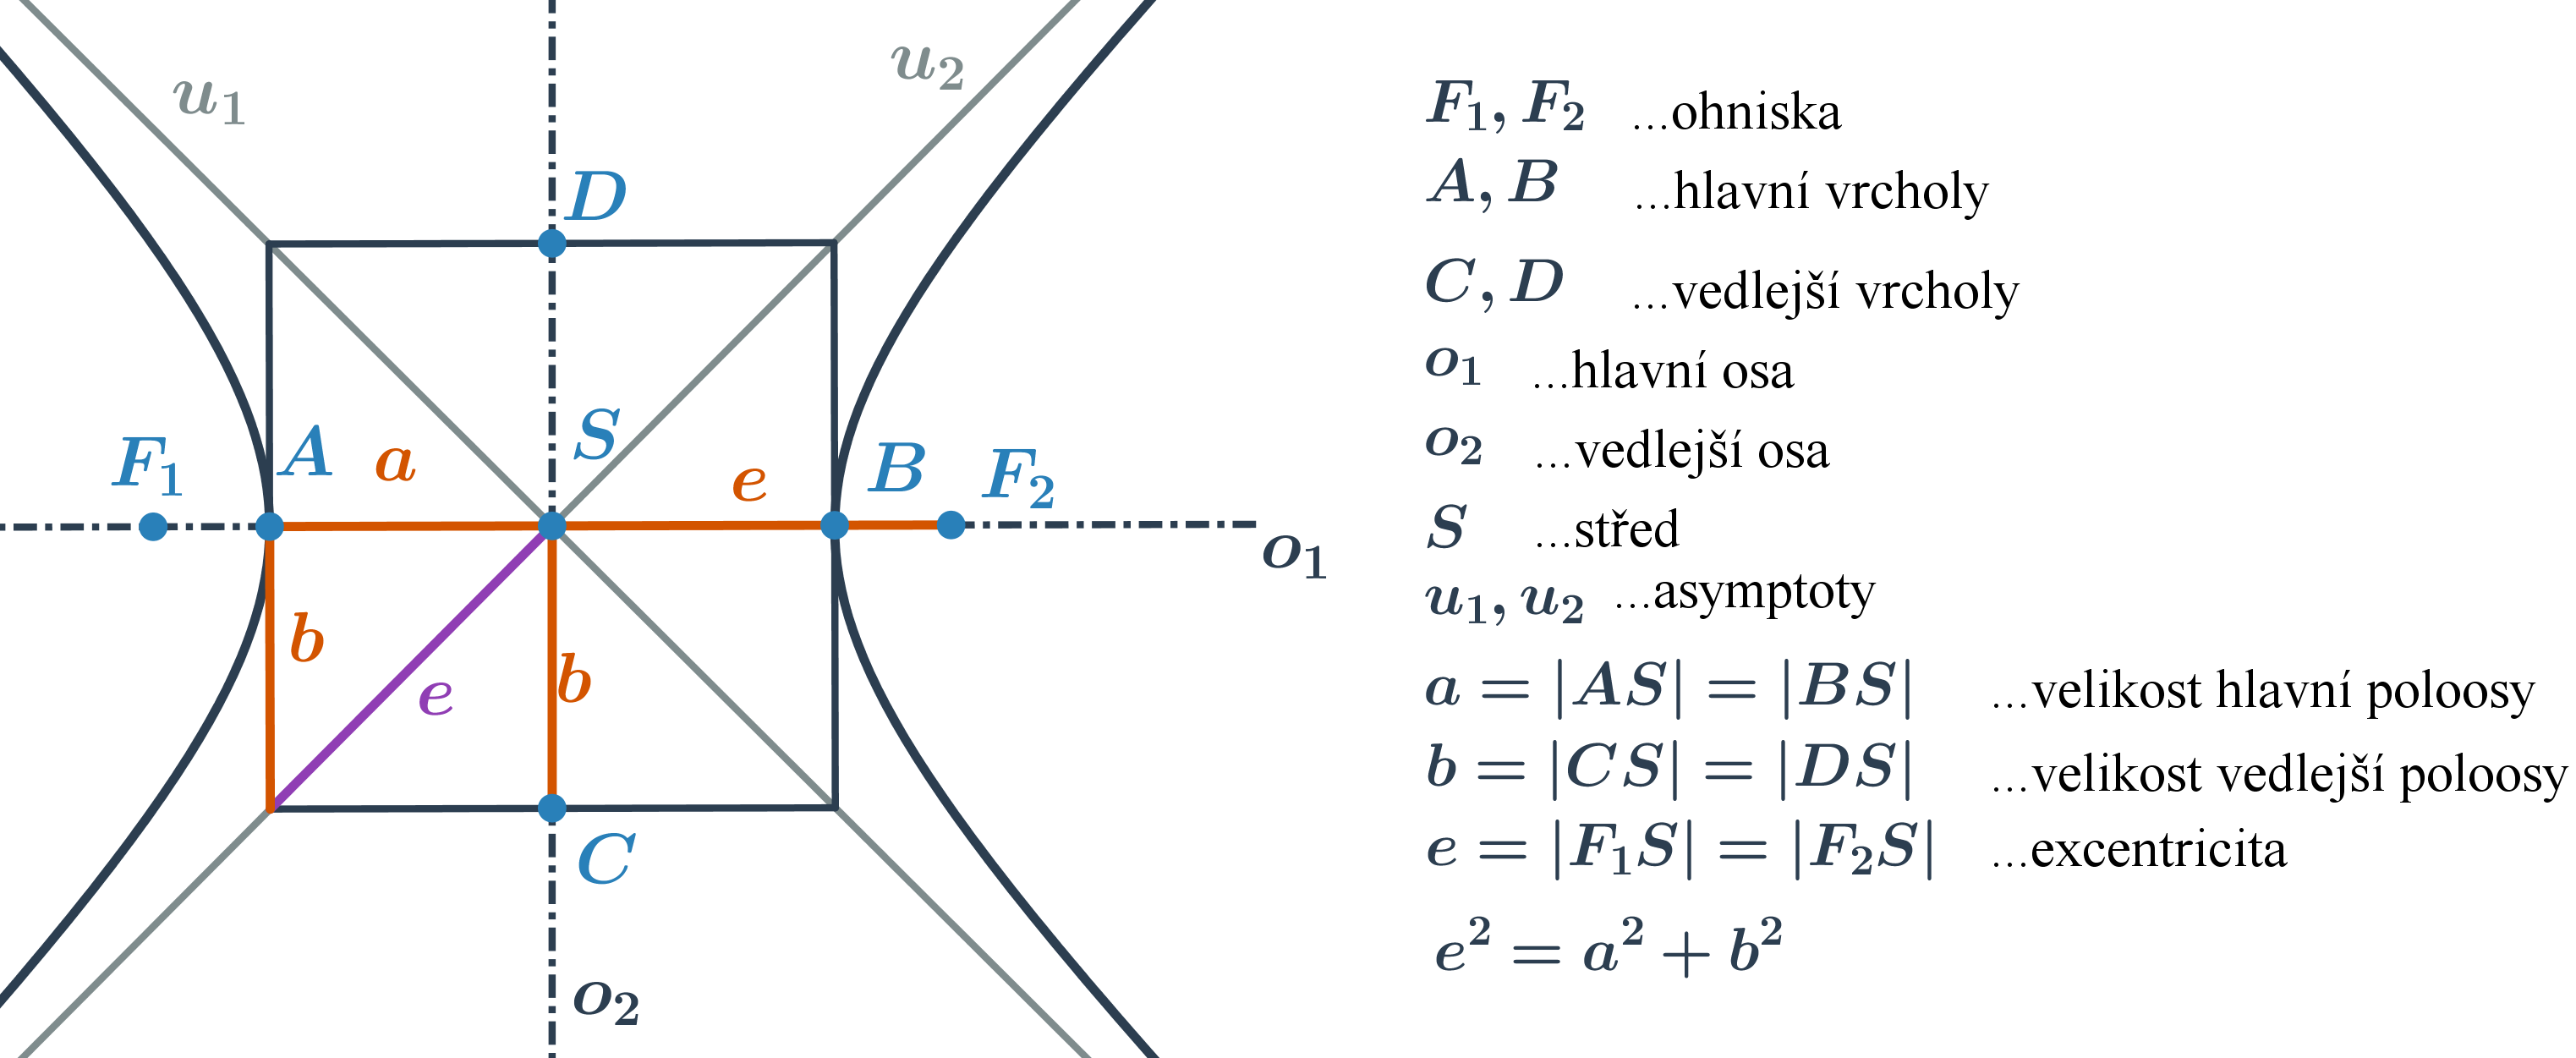
\includegraphics[width=0.7\linewidth]{img/14_hyperbola1.png}
\subsection {Středová, vrcholová a obecné rovnice}
    Obecnou rovnici kuželosečky získáme ze středové rovnice provedením operací ve středové rovnici a zavedením nových konstant\\
    Středovou rovnici kuželosečky získáme z obecné rovnice doplněním na čtverec
\subsubsection{Parabola}
    Obecná rce paraboly je: $y^2 + 2rx +2sy+t=0$ \\ 
 
    Je-li V[0;0]$2p>0$, $d= -\frac{p}{2}$ a $F[\frac{p}{2};0]$ vrcholová rovnice paraboly je: $y^2=2px$ \\
    Je-li V[0;0]$2p>0$, $d= \frac{p}{2}$ a $F[-\frac{p}{2};0]$ vrcholová rovnice paraboly je: $y^2=-2px$ \\
    Je-li V[0;0]$2p>0$, $d= -\frac{p}{2}$ a $F[0;\frac{p}{2}]$ vrcholová rovnice paraboly je: $x^2=2py$ \\
    Je-li V[0;0]$2p>0$, $d= -\frac{p}{2}$ a $F[0;-\frac{p}{2}]$ vrcholová rovnice paraboly je: $x^2=-2py$ \\

    Je-li V$[m,n]$, polopč. $VF$ a kladná poloosa x souhlasně orientované, a je omezené zleva je vrcholová rce. paraboly $(y-n)^2=2p(x-m)$\\
    Je-li V$[m,n]$, polopč. $VF$ a kladná poloosa x nesouhlasně orientované, a je omezená zprava je vrcholová rce. paraboly $(y-n)^2=-2p(x-m)$\\
    Je-li V$[m,n]$, polopč. $VF$ a kladná poloosa y souhlasně orientované, a je omezená zespoda je vrcholová rce. paraboly $(x-m)^2=2p(y-n)$\\
    Je-li V$[m,n]$, polopč. $VF$ a kladná poloosa y souhlasně orientované, a je omezená shora je vrcholová rce. paraboly $(x-m)^2=-2p(y-n)$\\
    Obecná rce paraboly je: $y^2 + 2rx +2sy+t=0$ \\
   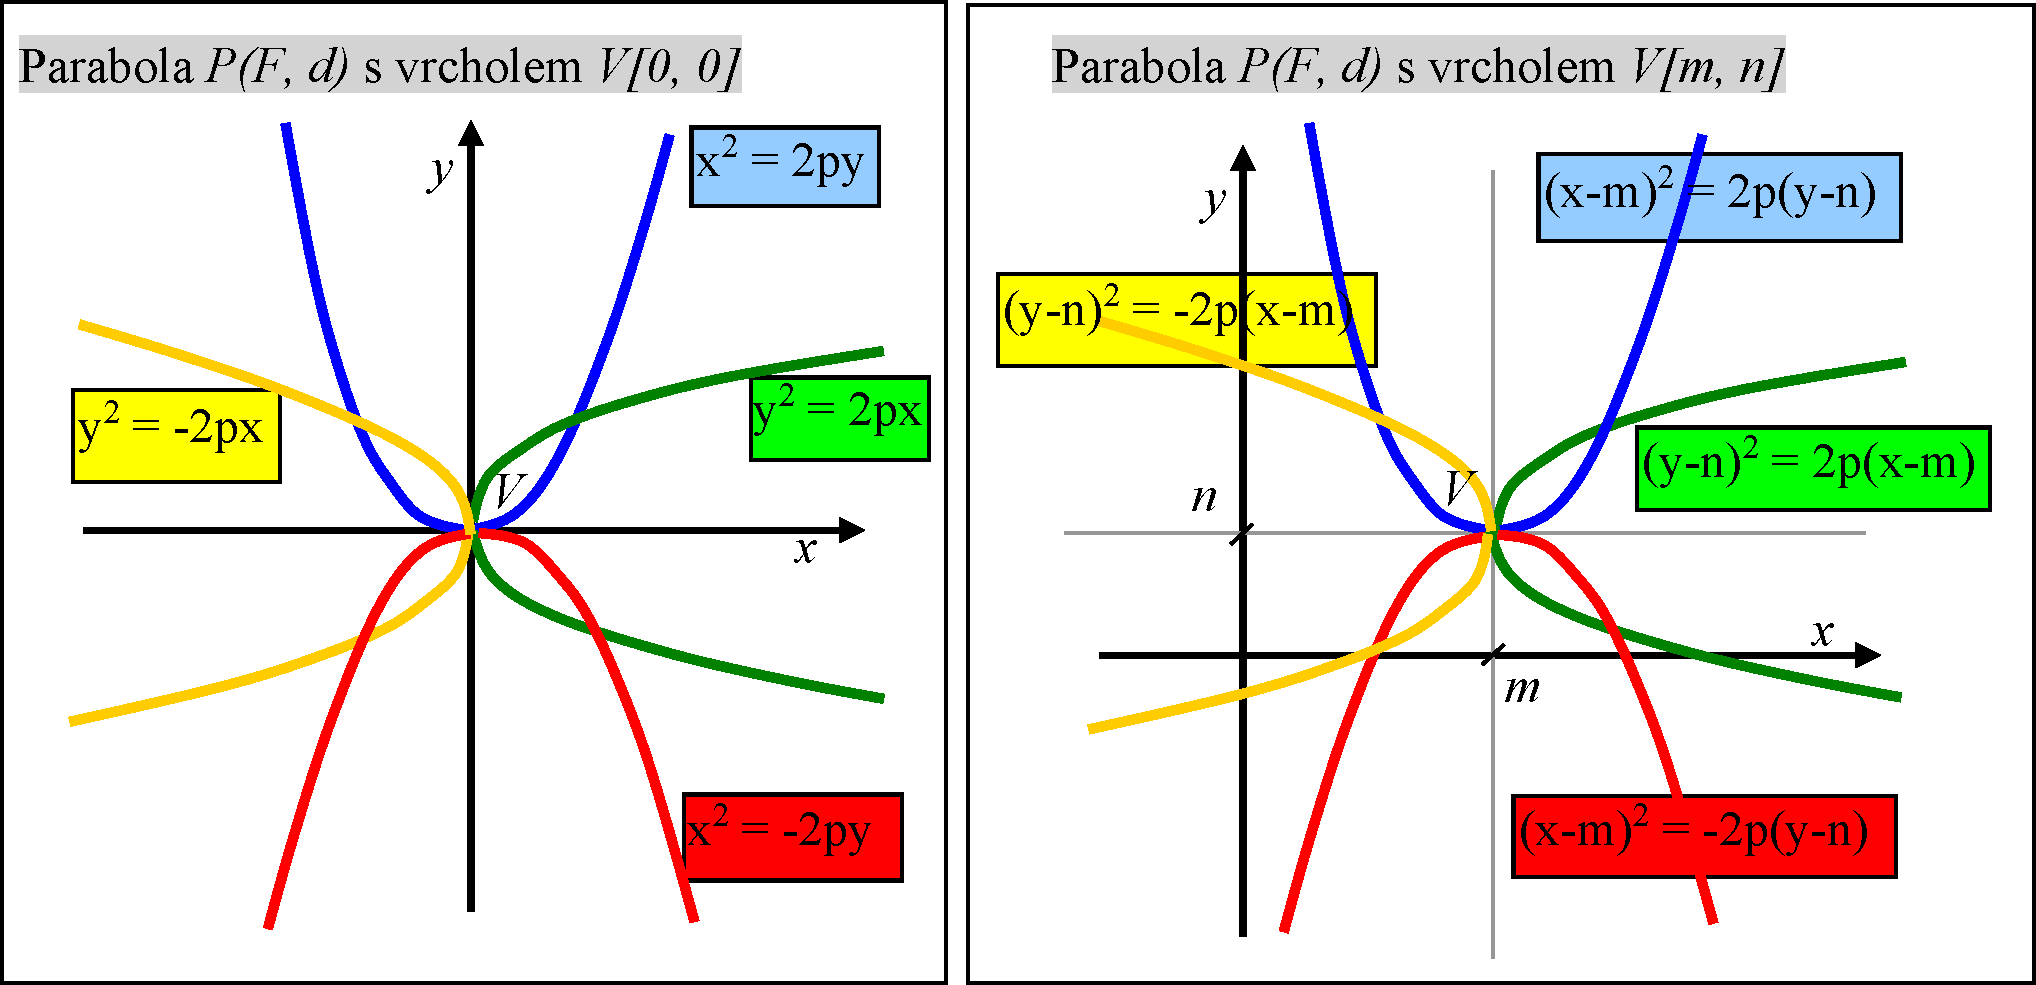
\includegraphics[width=0.8\linewidth]{img/14_parabola2.png}

\subsubsection{Hyperbola}
    Obecná rce hyperboly je: $px^2+qy^2+2rx+2sy+t=0$, kde $pq<0$ (jedno je záporné) 

    Jeli S[0;0] a hyperbola je umístěna horizontálně, je F[$-e$;0] a G[$e$;0],$a$ je hlavní poloosa a $b$ je vedlejší poloosa pak středová rovnice hyperboly je  $\frac{x^2}{a^2} - \frac{y^2}{b^2}=1$\\ 
    Jeli S[0;0] a hyperbola je umístěna vertikálně, je F[0, $e$] a G[0, $-e$] $a$ je hlavní poloosa a $b$ je vedlejší poloosa pak středová rovnice hyperboly je  $-\frac{x^2}{a^2} + \frac{y^2}{b^2}=1$\\
   
    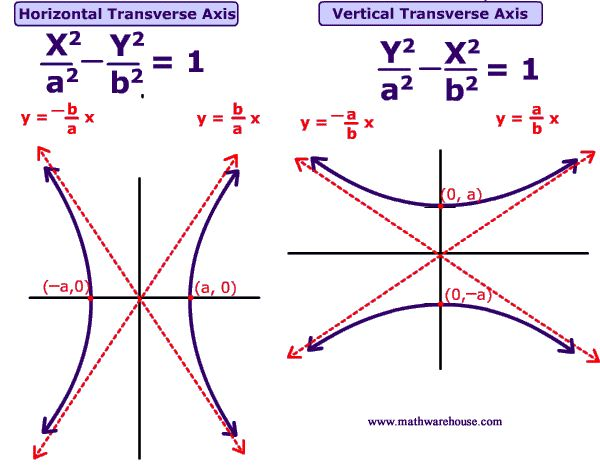
\includegraphics[width=0.5\linewidth]{img/14_hyperbola2.jpg}\\
    
    \vspace{1em}
    Je-li $S[m;n]$ a hlavní osa $o$ rovnoběžná s osou x je středová rovnice hyperboly: $\frac{(x-m)^2}{a^2} - \frac{(y-n)^2}{b^2}=1$, asymptoty mají tvar $a_1,2: (y-n)=\pm \frac{b}{a}(x-m)$
    Je-li $S[m;n]$ a hlavní osa $o$ rovnoběžná s osou y je středová rovnice hyperboly: $-\frac{(x-m)^2}{a^2} + \frac{(y-n)^2}{b^2}=1$, asymptoty mají tvar $a_1,2: (y-n)=\pm \frac{a}{b}(x-m)$
    
\subsection{Vzájemná poloha kuželosečky a bodu}
    Nechť je dána obecná rovnice kuželosečky a bod $A[x_A,y_A]$. Označíme si levou stranu obecné rovnice kuželosečky $f(x,y)$ pro každý bod kuželosečky a dosadíme souřadnice bodu $A[x_A,y_A]$ a pro jednotlivé kuželosečky platí: \begin{itemize}
        \item $A$ je bodem kuželosečky právě tehdy když $f(x_A,y_a)=0$
        \item $A$ je vnějším bodem kuželosečky právě když $f(x_A,y_a)>0$
        \item $A$ je vnitřním bodem kuželosečky právě když $f(x_A,y_a)<0$
    \end{itemize}
\subsection{Vzájemná poloha kuželosečky a přímky}
    Vzájemnou polohu kuželosečky a přímky určujeme tak, že hledáme jejich společné body. Analyticky to znamená, že hledáme řešení soustavy lineární rce (přímka) a kvadratické rce (kuželosečka) o dvou neznámých. To nakonec vede k řešení kvadratické rce o jendé neznáme. Ta může mít: \begin{itemize}
        \item Pro $D>0$ - dva společné body tj. sečna
        \item Pro $D=0$ - jedno řešení tj. tečna nebo i sečna (u paraboly, pokud přímka je rovnoběžná s osou)!
        \item Pro $D<0$ - žádné řešení tj. vnější přímka
    \end{itemize}
\subsection{Vzájemná poloha kuželoseček}
    Vzájemná poloha kuželoseček se zkoumá opět tak, že se hledají společné body, analyticky to znamená, že se řeší soustava dvou kvadratických rovnic o dvou neznámých
\title{17. Objemy a povrchy těles, řezy těles rovinou}

\author{Jan Peroutka}
\maketitle

\section{Objemy a povrchy těles, řezy těles rovinou}

\subsection{Obecně k tělesům}
Tělesa jsou trojrozměrné geometrické útvary, jejichž objem a povrch se dá vyjádřit pomocí matematických vzorců. Dále je lze zobrazit a analyzovat pomocí řezů rovinou.

\subsection{Hranol}
\begin{itemize}
    \item Objem: $V = S_p \cdot v$, kde $S_p$ je obsah podstavy a $v$ výška.
    \item Povrch: $S = 2 \cdot S_p + S_{pl}$, kde $S_{pl}$ je obsah pláště (součet obsahů stěn mezi podstavami).
\end{itemize}
\textbf{Řezy hranolem:} mohou být rovnoběžné s podstavou (vypadá jako podstava), nebo kolmé na podstavu (obdélníky nebo pravoúhlé tvary).

\subsection{Válec}
\begin{itemize}
    \item Objem: $V = \pi r^2 v$
    \item Povrch: $S = 2\pi r^2 + 2\pi r v$
\end{itemize}
\textbf{Řezy válcem:}
\begin{itemize}
    \item Řez rovinou rovnoběžnou s osou: obdélník
    \item Řez kolmý na osu: kruh
\end{itemize}

\subsection{Kužel}
\begin{itemize}
    \item Objem: $V = \frac{1}{3} \pi r^2 v$
    \item Povrch: $S = \pi r^2 + \pi r s$, kde $s$ je délka strany (tvořící).
\end{itemize}
\textbf{Řezy kuželem:}
\begin{itemize}
    \item Kolmý řez osou: rovnoramenný trojúhelník
    \item Rovnoběžný s podstavou: kruh menšího poloměru
\end{itemize}

\subsection{Koule}
\begin{itemize}
    \item Objem: $V = \frac{4}{3} \pi r^3$
    \item Povrch: $S = 4\pi r^2$
\end{itemize}
\textbf{Řezy koulí:} libovolný rovinný řez koulí je kruh. Největší řez (středový) je kruh s poloměrem $r$.

\subsection{Poznámka k řezům}
Řezy těles nám pomáhají pochopit jejich vnitřní strukturu. Často se využívají např. v technických výkresech, deskriptivní geometrii nebo fyzice.

\subsubsection*{Konstrukční pravidla pro rýsování řezu hranolem}

\begin{enumerate}
    \item \textbf{Dva body leží na stejné stěně} $\Rightarrow$ \emph{spojujeme je přímou úsečkou.}  
    Pokud zadané body leží na téže stěně tělesa, můžeme je přímo spojit úsečkou. Tato úsečka pak tvoří část řezu.

    \item \textbf{Tři body, z nichž dva leží na jedné stěně a třetí na protější} $\Rightarrow$ \emph{určíme směr a vedeme rovnoběžku.}  
    Například body $A$ a $B$ leží na přední stěně, bod $C$ na zadní: spojíme $A$ a $B$, čímž určíme směr, a tímto směrem vedeme rovnoběžku přes bod $C$.

    \item \textbf{Dva body leží ve dvou různých stěnách, třetí leží ve třetí stěně} $\Rightarrow$ \emph{určíme průsečík pomocí roviny.}  
    Pokud body $L,J$ a $K$ leží ve dvou různých stěnách (např. přední a boční), určíme rovinu jejich spojením. Tato rovina protne třetí stěnu (např. pravou) – najdeme průsečík této roviny s hranou dané stěny (např. $BF$) a tím získáme další bod (např. $M$). Pokud třetí bod (např. $K$) už leží v této rovině, lze ho rovnou použít a spojit s ostatními.

    \begin{figure}
        \centering
        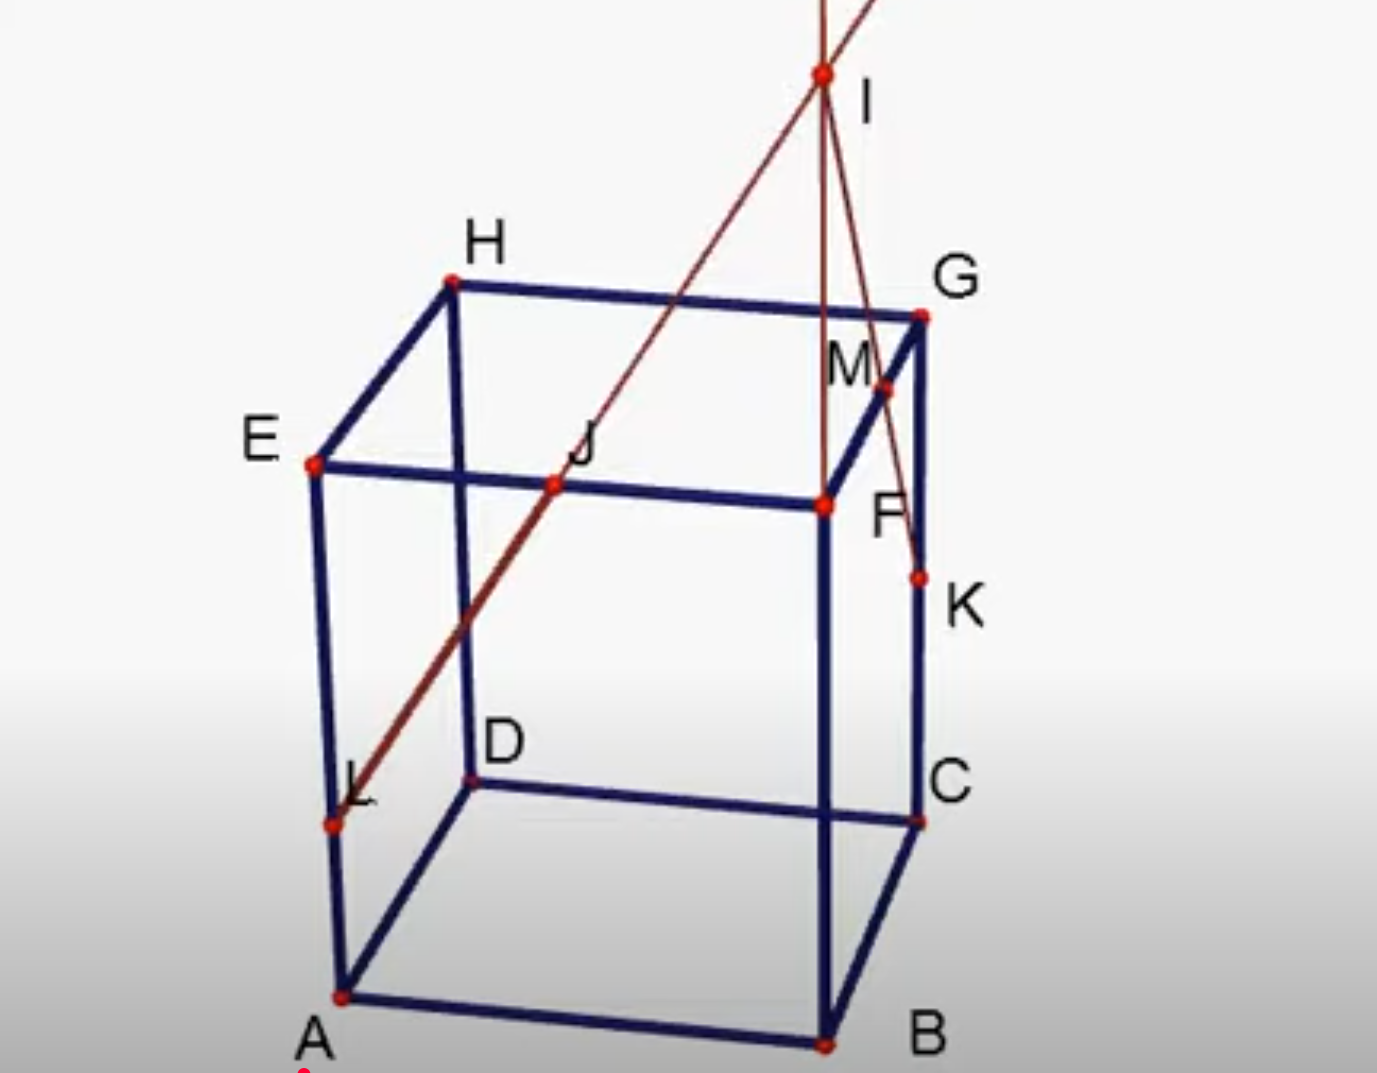
\includegraphics[width=0.5\linewidth]{img/16_objemy_rez.png}
        \caption{3. pravidlo v akci}
    \end{figure}

    \item \textbf{Řezová čára je vždy spojitá a tvořená úsečkami.}  
    Musí ležet v jednotlivých stěnách tělesa a nesmí se „lámat“ uvnitř jedné stěny.

    \item \textbf{Řez vždy začíná a končí na hraně tělesa.}  
    Žádná část řezu nesmí ležet mimo stěnu nebo končit „ve vzduchu“.

    \item \textbf{Rovina řezu nemůže částečně ležet v hraně – buď celá, nebo vůbec.}  
    Pokud rovina řezu prochází hranou, musí celá ležet v rovině této stěny.
\end{enumerate}

\title{18. Tečny k funkcím a kuželosečkám}
\author{Jakub Švagr}
\date{2.5.2025}

\maketitle

\section{Tečna}
Tečna je přímka, která má k dané funkci nebo kuželosečce v určitém bodě stejný směrový vektor (směrnici), jako ta funkce nebo kuželosečka. Tečna leží vně (venku) funkce, až na jeden společný bod, který sdílí s funkcí.

\subsection{Normála}
Normála je přímka kolmá na tečnu, která prochází bodem dotyku. Rovnice normály se získá z rovnice tečny změnou směrnice na její zápornou převrácenou hodnotu.
\[
Ax + By + C = 0
\]

\begin{itemize}
  \item \( A, B, C \) jsou reálné konstanty
  \item pokud \( B \neq 0 \), můžeme tvar převést do směrnicového
  \item směrnice přímky je potom \( k = -\frac{A}{B} \)
\end{itemize}

\subsection{Směrnice}
Směrnice přímky je tangens úhlu, který daná přímka svírá s kladnou poloosou x.
\[
y = kx + q
\]
\begin{itemize}
  \item \( k \) je směrnice přímky – určuje její sklon přímky,
  \item \( q \) je absolutní člen – určuje průsečík přímky s osou \( y \)
\end{itemize}

\subsection{Jak na to?}

\subsubsection{Tečna k funkci}
U funkcí hledáme tečnu pomocí derivace. Derivace funkce v bodě udává hodnotu směrnice tečny.
\begin{enumerate}
\item Máme funkci \( f(x) = \frac{2x + 1}{x^2} \), chceme najít rovnici tečny v bodě \( T[-2; ?] \).

\item Nejdříve spočítáme funkční hodnotu tím, že za x dosadíme -2:

\[
f(-2) = \frac{2 \cdot (-2) + 1}{(-2)^2} = \frac{-4 + 1}{4} = \frac{-3}{4}
\]

Bod dotyku je tedy \( T[-2; -\frac{3}{4}] \).

\item Nyní funkci zderivujeme, tím získáme:

\[
f'(x) = \frac{2x^2-(2x+1)2x}{x^4}= \frac{2x(x-(2x+1))}{x^4}= \frac{2(-x-1)}{x^3}= \frac{-2(1+x)}{x^3}
\]

\item Dosadíme \( x = -2 \) do zderivované funkce:

\[
f'(x) = -\frac{2([-2]+1)}{(-2)^3} = -\frac{-2}{-8} = -\frac{1}{4}
\]

\item Tečna má tedy směrnici \( -\frac{1}{4} \), bodem \( T[-2; -\frac{3}{4}] \) vede tečna s rovnicí:
\[
y = -\frac{1}{4}x +c 
\]
dosadíme za souřadnice x a y
\[
-\frac{3}{4} = -\frac{1}{4}(-2) +c 
\]
\[
-\frac{3}{4} = \frac{1}{2} +c 
\]\[
-\frac{5}{4} =c 
\]
dosadíme vypočítané $c$ do rovnice a máme rovnici tečny funkce v daném bodě
\[
y = -\frac{x}{4} - \frac{5}{4} 
\]
\end{enumerate}
    \begin{figure}[h]
        \centering
        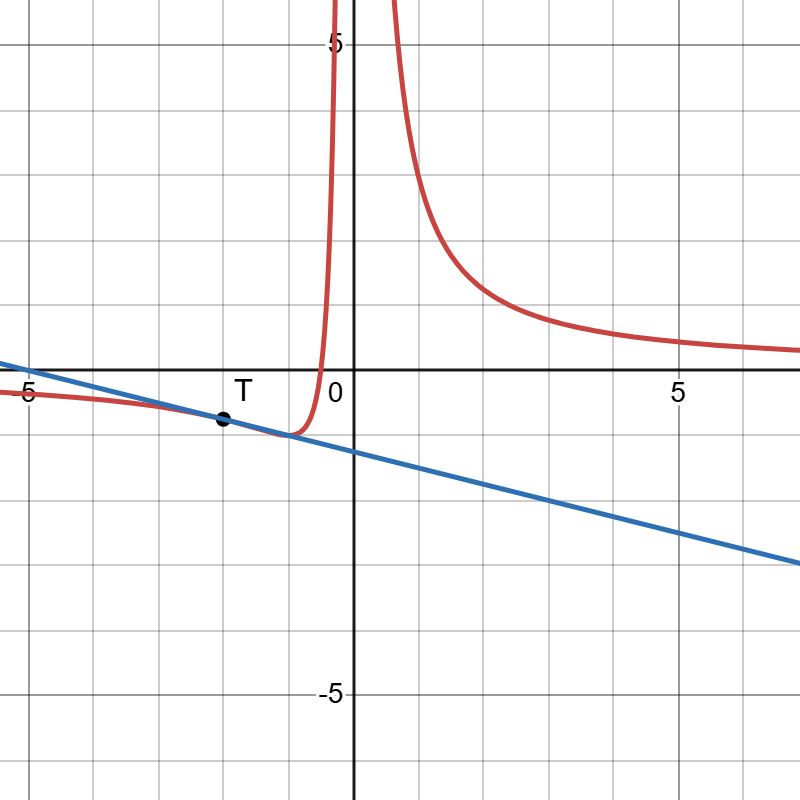
\includegraphics[width=0.5\linewidth]{img/17_Tecna_k_funkci.png}
        \caption{Tečna k funkci \(f(x) = \frac{2x + 1}{x^2}\)}
        \label{fig:enter-label}
    \end{figure}
\subsubsection{Tečna ke kuželosečce}
U kuželoseček hledáme tečnu pomocí soustavy rovnic a diskriminantu. Pokud dosadíme rovnici přímky do rovnice kuželosečky, vznikne kvadratická rovnice. Tečna nastane tehdy, pokud má tato rovnice právě jedno řešení, tedy diskriminant je roven nule (neplatí pro parabolu, kdy sečna může mít jeden společný bod s kuželosečkou, pokud je rovnoběžná s osou).

\begin{enumerate}
\item Máme rovnici paraboly a přímku p, počítá se to jako soustava rovnic:
\[
P: y^2 - 16x - 4y - 12 = 0
\]
\[
p: x - y + c = 0
\]
\item Vyjádřeme si to, co pro nás bude lehčí, v tomto případě je to celkem jedno, ale zvolil jsem \(x\).
\[x = y - c\]

\item Dosadíme \( x \) z přímky do rovnice kuželosečky:

\[
y^2 - 16(y - c) - 4y - 12 = 0
\]
\[
y^2 - 16y + 16c - 4y -12 = 0
\]
\[
y^2 - 20y + 16c - 12 = 0
\]

\item Aby to byla tečna, kvadratická rovnice musí mít právě jedno řešení, tedy diskriminant \( D \) musí být roven nule:

\[
D = (-20)^2 - 4 \cdot 1 \cdot (16c - 12) = 400 - 64c + 48 = 448 - 64c
\]

\[
448 - 64c = 0 
\]
\[
c = \frac{448}{64} = 7
\]

\item Hodnota \( c = 7 \), naše tečna je tedy \( x - y + 7 = 0 \).
\end{enumerate}
\begin{figure}[h]
    \centering
    \includegraphics[width=0.3\linewidth]{img/17_Tecna_k_parabole.png}
    \caption{Tečna k parabole \(P: y^2 - 16x - 4y - 12 = 0\)}
    \label{fig:enter-label}
\end{figure}
\textbf{POZOR!} U paraboly nestačí, aby diskriminant byl nulový, protože se může stát, že přímka s kuželosečkou má právě jeden společný bod, ale není tečnou, ale sečnou. Toto se stane pokud je naše přímka kolmá na řídící přímku paraboly.
\subsubsection{Tečna u kuželoseček pokud máme bod doteku}
Existuje i jiná cesta, jak získat tečnu ke kuželosečce, a to pomocí vzorečků, zde je tabulka:
\begin{table}[h]
    \centering
    \begin{tabular}{|c|c|c|}
        \hline
        \textbf{Kuželosečka} & \textbf{Středová rovnice kuželosečky} & \textbf{Rovnice tečny v bodě $[x_0, y_0]$} \\ \hline
        Kružnice & $(x - m)^2 + (y - n)^2 = r^2$ & $(x_0 - m)(x - m) + (y_0 - n)(y - n) = r^2$ \\ \hline
        Elipsa & $\frac{(x - m)^2}{a^2} + \frac{(y - n)^2}{b^2} = 1$ & $\frac{(x_0 - m)(x - m)}{a^2} + \frac{(y_0 - n)(y - n)}{b^2} = 1$ \\ \hline
        Parabola & $(x - m)^2 = 2p(y - n)$ & $((y_0 - n)(y - n)=2p[(x - m)+(x_0 - m)])$ \\ \hline
        Hyperbola & $\frac{(x - m)^2}{a^2} - \frac{(y - n)^2}{b^2} = 1$ & $\frac{(x_0 - m)(x - m)}{a^2} - \frac{(y_0 - n)(y - n)}{b^2} = 1$ \\ \hline
    \end{tabular}
    \caption{Přehled rovnic kuželoseček a jejich tečen}
    \label{tab:kuželosečky}
\end{table}
\begin{enumerate}
\item Zde stačí pouze do rovnice dát souřadnice bodu doteku. Vezměme si rovnici paraboly. Toto je, mimochodem, ta stejná parabola, přepsaná v do středového útvaru.
\[
(y - 2)^2=16(x+1)
\]

\item Určeme si souřadnice středu a parametr, pro přehlednost:
\[
(y - 2)^2 = 16(x+1), 
m=-1,\;n=2,\;2p=16\;\Longrightarrow\;p=8
\]
\item Vezměme si rovnici z tabulky:
\[
(y_0 - n)(y - n) = p\bigl[(x-m)+(x_0-m)\bigr]
\]
\item Dosadíme do ní naše hodnoty:
\[
(10-2)(y-2) = 8\bigl[(x+1)+(3+1)\bigr]
\]
\item Pak to upravíme a dostaneme toto:
\[
8(y-2) = 8(x+5)
\]
\[
y-2 = x+5
\]
\[
x - y + 7 = 0
\]
\end{enumerate}
\title{19. Průběh funkce}
\author{Jakub Sláma}
\date{26.4.2025}

\maketitle

\section{Průběh funkce}
Vyšetřování průběhu funkce má několik kroků, následuje jejich seznam a popis:
\begin{enumerate}
    \item 
        \begin{itemize}
            \item Definiční obor 
            \item sudost nebo lichost
            \item periodičnost
        \end{itemize}
    \item
        \begin{itemize}
            \item jednostranné limity v bodech, kde není funkce definována
            \item limity v nevlastních bodech
        \end{itemize}
    \item
        \begin{itemize}
            \item průsečíky s osami x a y
            \item znaménka funkčních hodnot
        \end{itemize}
    \item
        \begin{itemize}
            \item první derivace, první derivace rovna 0, kde není definována
            \item intervaly monotónnosti, stacionární body
        \end{itemize}
    \item
        \begin{itemize}
            \item druhá derivace, druhá derivace rovna 0, kde není definována
            \item intervaly konvexnosti (nad tečnou) a konkávnosti (pod tečnou), extrémy, inflexní body
        \end{itemize}
    \item
        \begin{itemize}
            \item asymptoty bez směrnice $x=a$
            \item asymptoty se směrnicí $y=ax+b$
        \end{itemize}
    \item
        \begin{itemize}
            \item graf funkce
            \item obor hodnot
        \end{itemize}
\end{enumerate}

Vyšetřujeme funkci: 
$$
    f: y=\frac{x}{x^2+1}
$$
\subsection{Definiční obor, sudost nebo lichost, periodičnost}
\subsubsection{Obor hodnot}
Obor hodnot získáme zjištěním hodnot, které mohou být dosazeny za $x$.
V našem případě $D(f) \in R$
\subsubsection{Zjištění sudosti}
Funkce $f(x)$ je sudá, pokud platí:
$$
    f(-x)=f(x)
$$
(pokud se skládá z sudých funkcí a konstant) \\
Typickými sudími funkcemi je funkce kvadratická, nebo kubická.
\subsubsection{Zjištění lichosti}
Funkce $f(x)$ je lichá, pokud platí:
$$
    f(-x)=-f(x)
$$
(pokud se skládá z lichých funkcí a konstant)\\
\subsubsection{Periodičnost}
Funkce je periodická za předpokladu, že její průběh periodicky opakuje. Zástupci jsou například: $\sin(x); \cos(x); \tan(x); \cot(x)$
\subsubsection{Výpočet}
v našem případě:
$$
    f(-x)=\frac{-x}{(-x)^2+1}
$$

$$
    -\frac{x}{x^2+1}=\frac{-x}{(-x)^2+1}
$$
$$
    f(-x)=-f(x)
$$
při porovnání funkce po úpravách zjistíme, že je funkce lichá
\subsection{Limity vlastní a nevlastní}
Je nutno spočítat limity ve všech krajních bodech těch intervalů, které tvoří
definiční obor funkce $f$, pokud v nich tato funkce není přímo definovaná. Tj. jde většinou o jednostranné limity. Speciálně půjde často o limity v $+\infty; -\infty$
\\ \\
Např. v intervalech $(-\infty; 0)(0; \infty)$ rovnice $y=\frac{1}{x}$
$$
    \lim_{x\rightarrow0}{\frac{1}{x}}=0
$$
+ limity jdoucí do +, - nekonečna
\subsubsection{Jednostranné limity v bodech, kde není funkce definována}
Jednostranná limita je v infinitezimálním počtu libovolná z limit funkce $f(x)$ reálné proměnné $x$, u nichž se $x$ přibližuje k zadanému bodu buď zleva nebo zprava
\subsubsection{Limity v nevlastních bodech}
Limity v nevlastních bodech se týkají situací, kdy proměnná 
$x$ směřuje k nekonečnu nebo minus nekonečnu.
\subsubsection{Výpočet}
u této funkce $D(f) \in \mathbb{R}$, tudíž počítáme pouze limity jdoucí do +, - nekonečna  

$$
    \lim_{x\rightarrow\infty}{\frac{x}{x^2+1}}=0
$$
$$
    \lim_{x\rightarrow-\infty}{\frac{x}{x^2+1}}=0
$$

Tato funkce se blíží z obou stran k nule .
\subsection{Průsečíky s osami $x$ a $y$, znaménka funkčních hodnot}
\subsubsection{Průsečíky s osami $x$ a $y$}
Průsečíky s osami hodnot získáme dosazením 0 nejprve za $x$ souřadnici, poté za $y$
\subsubsection{Znaménka funkčních hodnot}
Za pomocí nulových bodů si vytvoříme tabulku, ve které zjistíme v kterých intervalech je funkce kladná a v kterých je záporná
\subsubsection{Výpočet}
1. výpočet průsečíku s osou $x$ ($y=0$)
$$
    0=\frac{x}{x^2+1}
$$
$$
    0=x
$$
souřadnice průsečíku funkce s osou x je $X[0;0]$ \\
2. výpočet průsečíku s osou $y$ ($x=0$)
$$
    y=\frac{0}{0^2+1}
$$
$$
    y=0
$$
souřadnice průsečíku funkce s osou y je $Y[0;0]$

$$
\begin{array}{|c|c|c|c|}
\hline
\textbf  & (-\infty;0\rangle & (0; \infty) \\
\hline
x     & - & + \\
x^2+1 & + & + \\
\hline
 & - & + \\
\hline
\end{array}
$$
Funkce v intervalu nabývá záporné hodnoty $(-\infty;0\rangle$ a v intervalu $(0; \infty)$ nabývá kladné hodnoty.

\subsection{První derivace, první derivace rovna 0, kde není definována, intervaly monotónnosti, stacionární body}
\subsubsection{První derivace, první derivace rovna 0, kde není definována}
První derivací zjistíme v kterých intervalech je funkce rostoucí, nebo klesající\\ \\
Pokud položíme první derivaci funkce rovnou nule body podezřelé z lokálních minim a maxim. \\ \\
Derivace také nemusí být definovaná, pokud má v nějakém bodě: \\
1. Nevlastní limitu (např. asymptotu) \\ 
2. Ostrý zlom (např. absolutní hodnota $y=|x|$ v bodě $x=0$)

\subsubsection{Intervaly monotónnosti, stacionární body}
Interval monotónnosti je část definičního oboru funkce, kde funkce buď stále roste, nebo stále klesá\\ \\
Stacionární bod je bod na grafu funkce, kde je první derivace rovna nule: $f'(x) = 0$ Funkce v tomto bodě může mít extrém (maximum, minimum)

\subsubsection{Výpočet}
nejprve zderivujeme výraz
$$
    f: y=\frac{x}{x^2+1} 
$$\\
$$
    y'=\frac{1(x^2+1)-x(2x)}{(x^2+1)^2}= \frac{x^2+1-2x^2}{(x^2+1)^2}=\frac{-x^2+1}{(x^2+1)^2}
$$\\
Následně výraz dáme roven 0, tímto zjistíme stacionární body
$$
    \frac{-x^2+1}{(x^2+1)^2} = 0
$$
Jsou dva $[1;0];[-1;0]$, následně zjistíme v kterých intervalech je funkce rostoucí a v kterých klesající:
$$
\begin{array}{|c|c|c|c|}
\hline
\textbf  & (-\infty;-1\rangle&(-1;1) & \langle 1; \infty) \\
\hline
-x^2+1  &   -  & + & - \\
(x^2+1)^2  & + & + & +\\
\hline
 & - & + & - \\
\hline
\end{array}
$$
Z tohoto vylívá, že funkce je klesající v intervalech $(-\infty;-1\rangle \cup \langle 1; \infty)$ klesající a v intervalu $(-1;1)$ rostoucí. \\ \\
Musíme dosadit body monotónnosti do původní rovnice, aby jsme získali souřadnice minim a maxim.
$$
    f: y=\frac{x}{x^2+1} 
$$\\
pro $x = 1$
$$
    f: y=\frac{1}{1^2+1} =\frac{1}{2}
$$
Souřadnice maxima je $[1;\frac{1}{2}]$
pro $x = -1$
$$
    f: y=\frac{-1}{(-1)^2+1} =-\frac{1}{2}
$$
Souřadnice minima je $[1;-\frac{1}{2}]$

Minimum je mezi klesajícím a rostoucím intervalem. \\
Maximum je mezi rostoucím a klesajícím.

\subsection{Druhá derivace, druhá derivace rovna 0, kde není definována, intervaly konvexnosti (nad tečnou) a konkávnosti (pod tečnou), inflexní body}

\subsubsection{Druhá derivace, druhá derivace rovna 0, kde není definována,}
Pomocí druhé derivace zjistíme tvar křivky (konkávnost, konvexnost) za pomocí intervalů (v kladných je funkce konvexní (nad tečnou $\cup$), v záporných je konkávní (pod tečnou $\cap$))  \\
Druhou derivaci funkce pokládáme nule, aby jsme zjistily inflexní body (body, ve kterých se mění zakřivení grafu funkce) \\
druhá derivace není definována, pokud:
\begin{itemize}
    \item Funkce není dostatečně hladká – není spojitá nebo není dostatečně "plynulá"
    \item První derivace není spojitá – například má ostrý zlom.
    \item Výpočty vedou k dělení nulou – druhá derivace obsahuje problémové místo (asymptoty).
    \item Funkce sama není definovaná – např. odmocnina ze záporného čísla, dělení nulou apod.
\end{itemize}

\subsubsection{Intervaly konvexnosti (nad tečnou) a konkávnosti (pod tečnou), inflexní body}
Konkávnost a konvexnost určují tvar křivky v intervalech. \\
V kladných intervalech je funkce konvexní (nad tečnou $\cup$),\\ 
V záporných intervalech je konkávní (pod tečnou $\cap$) \\ \\
inflexní body- Inflexní body jsou body, kde se mění zakřivení grafu (nulové body druhé derivace)

\subsubsection{Výpočet}
Vypočítáme si druhou derivaci funkce:
$$
    y'=\frac{-x^2+1}{(x^2+1)^2}
$$\\
$$
    y''=\frac{-2x\cdot(x^2+1)^2-(-x^2+1)\cdot2(x^2+1)(2x)}{(x^2+1)^4}=
$$\\
$$
    =\frac{[-2x(x^2+1)][(x^2+1)+2(-x^2+1)]}{(x^2+1)^4}=
$$\\
$$
    =\frac{-2x(x^2+1-2x^2+2)}{(x^2+1)^3}=
$$\\
$$
    =\frac{2x(x^2-3)}{(x^2+1)^3}
$$
Položíme druhou derivaci rovnou nule a zjistíme inflexní body:
$$
    \frac{2x(x^2-3)}{(x^2+1)^3}=0
$$
Nulové body jsou: $-\sqrt{3};0,\sqrt{3} $, vytvoříme tabulku:

$$
\begin{array}{|c|c|c|c|c|}
\hline
\textbf  & (-\infty;-\sqrt{3}\rangle&(-\sqrt{3};0) & \langle 0; \sqrt{3}) & \langle \sqrt{3}; \infty) \\
\hline
x^2-3      &   +  & - & - &+\\
2x         &   -  & - & + &+\\
(x^2+1)^3  &   +  & + & + & +\\
\hline
 & - & + & - &+\\
 & \text{konkávní} & \text{konvexní} & \text{konkávní} & \text{konvexní}\\
 & \frac{}{\cap} & \frac{}{\cup} & \frac{}{\cap} & \frac{}{\cup}\\
 &  &  &  &\\
\hline
\end{array}
$$
Díky ní zjistíme tvar grafu funkce v intervalech. \\ 
vypočítáme si souřadnice inflexních bodů dosazením do původní rovnice:\\
$x=-\sqrt{3}$
$$
    f: y=\frac{-\sqrt{3}}{(-\sqrt{3})^2+1} =-\frac{\sqrt{3}}{4}
$$\\
$x=0$
$$
    f: y=\frac{0}{(0)^2+1} = 0
$$
$x=-\sqrt{3}$
$$
    f: y=\frac{\sqrt{3}}{(\sqrt{3})^2+1} =\frac{\sqrt{3}}{4}
$$\\

Inflexní body mají souřadnice: $[-\sqrt{3};-\frac{\sqrt{3}}{4}];[0;0];[-\sqrt{3};\frac{\sqrt{3}}{4}]$
\subsection{Asymptoty bez směrnice $x=a$, asymptoty se směrnicí $y=ax+b$}
Asymptota je rovnice přímky ke které se funkce blíží, ale nikdy ji neprotne. Dělíme je na asymptoty se směrnicí a bez směrnice.
\subsubsection{Asymptoty bez směrnice $x=a$}
Asymptota bez směrnice vzniká v bodech, které jsou vyjmuty z $D(f)$, nebo $H(f)$. Jejich předpisem je $x=a$, nebo $y=a$, kde $a \in R$
lze vypočítat, jako 
$$
    \lim_{x\to a^+} f(x)
$$nebo 
$$
    \lim_{x\to a^-} f(x)
$$ \\
Příklad:
$$
    f(x)=\frac{1}{x-2}
$$
funkce není definována v bodě $x=2$
limyty:
$$
    \lim_{x\to 2^-}\frac{1}{x-2}=-\infty
$$
$$
    \lim_{x\to 2^+}\frac{1}{x-2}=+\infty
$$
Takže $x=2$ je svislá asymptota


\subsubsection{Asymptoty se směrnicí $y=ax+b$}

\subsection{Graf funkce, obor hodnot, výsledek příkladu}
Graf funkce sestrojíme vynesením minim, maxim, inflexních bodů a jejich následným propojením pomocí konkávních a konvexních křivek v příslušných intervalech.

\begin{figure}[H]
        \centering
        \includegraphics[width=0.8\linewidth]{img/18_graf_po_vysetreni.png}
        \caption{Graf vyšetření funkce} 
        \label{fig:enter-label}
    \end{figure}

Z grafu můžeme vyčíst, že $H(f)$ se pohybuje mezi minimem a maximem, tudíž $H(f) \in \langle -\frac{1}{2}; \frac{1}{2} \rangle$



\title{20. Analytická geometrie lineárních útvarů, vektorová algebra}
\author{Michaela Dudašková (Jakub Sláma)}
\date{1.5.2025}

\maketitle

\section{Analytická geometrie lineárních útvarů, vektorová algebra}
- Používáme kartézskou soustavu souřadnic \\
- Bod X má souřadnice $[a,b]$, souřadnice a leží na ose $x$ a souřadnice $b$ leží na ose $y$ je to uspořádaná dvojice hodnot.\\
\begin{figure}[H]
        \centering
        \includegraphics[width=0.4\linewidth]{img/20_kartezka_souradnice.png}
        \caption{Graf kartézské soustavy souřadnic} 
        \label{fig:enter-label}
    \end{figure}

\subsection{Body a vektory}
Pro body $A[x_a;y_a];B[x_b;y_b]$:\\ \\
\subsubsection{Střed úsečky:} 
$$
    S[\frac{x_a+x_b}{2};\frac{y_a+y_b}{2}]
$$ 
\subsubsection{Velikost úsečky:} 
$$
    |AB|=\sqrt{(x_b-x_a)^2+(y_b-y_a)^2}
$$
\subsubsection{Orientovaná úsečka:}
\begin{itemize}
    \item Kromě délky určuje i směr
    \item Určuje počátek a konec
    \item Opačně orientované úsečky mají opačné hodnoty
\end{itemize}
$$
    \overrightarrow{AB}=B-A=(x_b-x_a;y_b-y_a)
$$
$$
    \overrightarrow{BA}=A-B=(x_a-x_b;y_a-y_b)
$$
\subsubsection{Vektor}
\begin{itemize}
    \item Všechny orientované úsečky se stejným směrem a velikostí
    \item Označují se malým písmenem a šipkou
    \item Zobrazují posunutí (o kolik se bod posunul po ose $x$ a $y$)
    \item Kolmé vektory mají hodnoty prohozené a u jedné odlišné znaménko
\end{itemize}
$$
    \overrightarrow{u}=(a;b)
$$
$$
    \overrightarrow{u} \perp \overrightarrow{v}
$$
$$
    \overrightarrow{v}=(b;-a)
$$
\subsubsection{Operace s vektory}
\begin{itemize}
    \item Můžeme násobit vektor libovolným číslem, musíme ale násobit obě souřadnice
    \item Můžeme sčítat a odčítat vektory

$$
    \overrightarrow{u}+\overrightarrow{v}=(x_u+x_v;y_u+y_v)
$$
$$
    \overrightarrow{u}-\overrightarrow{v}=(x_u-x_v;y_u-y_v)
$$
    \item Můžeme vektory násobit – skalární součin
$$
    \overrightarrow{u} \cdot \overrightarrow{v}=(x_u\cdot x_v;y_u\cdot y_v)
$$
\end{itemize}
\subsubsection{Odchylka vektorů (odchylka dvou přímek)}
\begin{itemize}
    \item Odchylka dvou přímek je od $0^\circ$do $90^\circ$- u vektorů neplatí
    \item Odchylka u vektorů je od $0^\circ$ do $180^\circ$ \\
$$
    cos\alpha=\frac{\overrightarrow{u} \cdot \overrightarrow{v}}{|\overrightarrow{u}| \cdot |\overrightarrow{v}|}
$$
    \item Úhel $0^\circ$ svírají dva rovnoběžné a stejně orientované vektory
    \item Úhel $180^\circ$ svírají rovnoběžné a opačně orientované vektory
    \item Rovnoběžné vektory poznáme tak, že jeden je násobek toho druhého
    \item Úhel $90^\circ$ svírají kolmé vektory — skalární součin musí být roven nule
    \item Tzv. Nulový vektor $\overrightarrow{0}=(0;0)$
\end{itemize}

\subsection{Přímky}

\subsubsection{Parametrická rovnice přímky}

\begin{itemize}
    \item Směrový vektor $\overrightarrow{u}$ určuje směr, je rovnoběžný s přímkou
    \item Parametr, který náleží do množiny reálných čísel: $ t \in \mathbb{R} $
    \item Bod $ A $, který leží na přímce
\end{itemize}
$$
    x\in p:x=x_a+t \cdot \overrightarrow{u_x}
$$
$$
    y\in p:y=y_a+t \cdot \overrightarrow{u_y}; t \in \mathbb{R}
$$

\subsubsection{Obecná rovnice přímky}

\begin{itemize}
    \item Alespoň jedno z čísel $a$, $b$, $c$ musí být nenulové, aby rovnice určovala přímku.
    \item Normálový vektor – kolmý na přímku, má souřadnice $(a, b)$.
    \item Bod ležící na přímce má souřadnice $[x, y]$, které splňují rovnici.
$$
    ax+by+c=0
$$
    \item Čísla $a$, $b$, $c$ by měla být nesoudělná (tj. jejich největší společný dělitel je 1).
\end{itemize}

\subsubsection{Směrnicový tvar přímky}
\begin{itemize}
    \item Směrnice = tangens úhlu mezi přímkou a kladnou poloosou $x$.
    \item Přímka rovnoběžná s osou $y$ nemá směrnicový tvar!
    $y=kx+q$
    $k=tg\alpha$
\begin{figure}[H]
        \centering
        \includegraphics[width=0.2\linewidth]{img/20_kartezka_alfa.png}
        \caption{Graf směrnicové přímky} 
        \label{fig:enter-label}
    \end{figure}
\end{itemize}

\subsubsection{Polopřímky}

\begin{itemize}
    \item Stačí u parametrické rovnice přímky zadat interval, ze kterého budeme parametr vybírat.
$p:$
$$
    x=a_x+t\cdot u_x
$$
$$
    x=a_y+t\cdot u_y; t \in (z;r)
$$
Kdy $z$ označuje začátek intervalu a $r$ konec. Intervaly mohou být otevřené i zavřené.
\end{itemize}

\subsubsection*{Bod a přímka}

\begin{itemize}
    \item Pro zjištění, zda bod leží na přímce, dosadíme souřadnice bodu za $x$ a $y$ do rovnice přímky.
    \item Vzdálenost bodu od přímky lze spočítat pomocí speciálního vzorce.
\end{itemize}
$$
    p: ax+by+c=0
$$
$$
    M=[m;n]
$$
$$
    V_{M,p}=\frac{|a\cdot m+b \cdot n + c|}{\sqrt{a^2+b^2}}
$$

\subsubsection{Vzájemná poloha dvou přímek v rovině}
\begin{itemize}
    \item Vzájemnou polohu zjistíme pomocí soustavy rovnic.
    \item Možnosti:
    \begin{itemize}
        \item \textbf{Totožné} – jedna rovnice je násobkem druhé, výsledkem je nekonečně mnoho společných bodů.
        \item \textbf{Rovnoběžné} – soustava nemá řešení, přímky se nikdy neprotínají.
        \item \textbf{Různoběžné} – soustava má právě jedno řešení, přímky se protínají v jednom bodě.
    \end{itemize}
\end{itemize}

\title{21. Vztahy geometrických útvarů v rovině - podobnost a stejnolehlost}
\author{Jonáš Lavička}
\date{1.5.2025}

\maketitle

\section{Vztahy geometrických útvarů v rovině\\- podobnost a stejnolehlost}
    \subsection{Definice}
        Dva geometrické útvary nazýváme podobné, jestliže poměry délek všech dvojic odpovídajících si úseček těchto útvarů se rovnají témuž číslu - koeficientu podobnosti.\\
        Podobnost zachovává velikost úhlů a poměr délek.\\
        → Podobné útvary mají stejný tvar(bez ohledu na velikost)
        
    \subsection{Koeficient podobnosti}
        Koeficient podobnosti je poměr vzdálenosti dvou bodů daného geometrického útvaru a vzdálenosti. odpovídajících dvou bodů jiného geometrického útvaru.\\
        Rovinné útvary $O_{1}$ a $O_{2}$ jsou podobné, píšeme:  $O_{1} \sim O_{2}$\\
        Vyjádření poměru podobnosti: $k = \left| X'Y' \right|:\left| XY \right| = \frac{\left| X'Y' \right|}{\left| XY \right|}$ ; $\left| X'Y' \right| = k \cdot \left| XY \right|$

    \subsection{Zvětšení - zmenšení}
        \begin{align*}
            & k>1   && \Rightarrow \text{podobný útvar je zvětšený}\\
            & 0<k<1 && \Rightarrow \text{podobný útvar je zmenšený}\\
            & k=1   && \Rightarrow \text{útvar je shodný}
        \end{align*}

    \subsection{Podobnost trojúhelníka}
        Trojúhelníky $\bigtriangleup ABC$ a $\bigtriangleup DEF$ jsou si podobné (píšeme $\bigtriangleup ABC \sim \bigtriangleup DEF$), pokud vyhoví jedné z následujících vět:
        \subsubsection{Věta sss}
            Každé dva trojúhelníky, které mají sobě rovné poměry délek všech tří dvojic odpovídajících stran, jsou si podobné.\\
            \[k=\frac{\left| DE \right|}{\left| AB \right|}=\frac{\left| EF \right|}{\left| BC \right|}=\frac{\left| DF \right|}{\left| AC \right|} \;\;\; \equiv \;\;\; k=\frac{a}{d}=\frac{b}{e}=\frac{c}{f}\]

            \begin{figure}[H]
                \centering
                \includegraphics[width=0.5\linewidth]{img/23_trojuhelniky_sss.png}
                \caption{Podobné trojúhelníky dle věty sss} 
                \label{fig:enter-label}
            \end{figure}
            
        \subsubsection{Věta sus}
            Každé dva trojúhelníky, které mají sobě rovné poměry délek dvou odpovídajících stran a shodují se v úhlu jimi sevřeném, jsou si podobné.
            \[k=\frac{\left| DE \right|}{\left| AB \right|}=\frac{\left| DF \right|}{\left| AC \right|} \;\;\; \cap \;\;\; \left| \measuredangle BAC\right| = \left| \measuredangle EDF \right|\]

            \begin{figure}[H]
                \centering
                \includegraphics[width=0.5\linewidth]{img/23_trojuhelniky_sus.png}
                \caption{Podobné trojúhelníky dle věty sus} 
                \label{fig:enter-label}
            \end{figure}
            
        \subsubsection{Věta uu}
            Každé dva trojúhelníky, které mají dva úhly stejné, jsou si podobné.\\
            
            \begin{figure}[H]
                \centering
                \includegraphics[width=0.5\linewidth]{img/23_trojuhelniky_uu.png}
                \caption{Podobné trojúhelníky dle věty uu} 
                \label{fig:enter-label}
            \end{figure}

        \subsubsection{Věta Ssu}
            Každé dva trojúhelníky, které mají sobě rovné poměry délek dvou odpovídajících stran a shodují se v úhlu naproti větší straně, jsou si podobné. Tento úhel je ostrý.
            \[k=\frac{\left| DE \right|}{\left| AB \right|}=\frac{\left| DF \right|}{\left| AC \right|} \;\;\; \cap \;\;\; \left| \measuredangle ABC\right| = \left| \measuredangle DEF \right|\]
            
            \begin{figure}[H]
                \centering
                \includegraphics[width=0.5\linewidth]{img/23_trojuhelniky_Ssu.png}
                \caption{Podobné trojúhelníky dle věty Ssu} 
                \label{fig:enter-label}
            \end{figure}
    \newpage
    \subsection{Věty vyplývající z podobnosti trojúhleníků}
        \begin{itemize}
            \item Dva trojúhelníky jsou podobné, jsou-li jejich odpovídající si strany rovnoběžné, nebo navzájem kolmé.
            \item Dva pravoúhlé trojúhelníky jsou podobné, shodují-li se v jednom ostrém úhlu nebo v poměru dvou odpovídajících si stran.
            \item Dva rovnoramenné trojúhelníky jsou podobné, shodují-li se v úhlu při základně nebo v úhlu při vrcholu.
            \item Každé dva rovnostranné trojúhelníky jsou si podobné.
        \end{itemize}
    
    \subsection{Stejnolehlost}
        Stejnolehlost neboli homotetie $H(S,\kappa)$ je podobné zobrazení určené bodem $S$ a nenulovým reálným číslem - koeficientem stejnolehlosti $\kappa$, ve kterém se zobrazí bod $X \neq S$ na bod $X'$ tak, že: $\left| X'S \right| = \left| \kappa \right| \cdot \left| XS \right|$\\
        Pro $\kappa > 0$ bod $X'$ leží na polopřímce $\mapsto SX$.\\
        Pro $\kappa < 0$ bod $X'$ leží na polopřímce opačné k $\mapsto SX$.\\

        \begin{figure}[H]
            \centering
            \includegraphics[width=0.5\linewidth]{img/23_stejnolehlost.png}
            \caption{Stejnolehlost s $\kappa>1$} 
            \label{fig:enter-label}
        \end{figure}
        
        Pro stejnolehlé zobrazení platí:
        \begin{itemize}
            \item Obrazem přímky je vždy přímka s ní rovnoběžná.
            \item Absolutní hodnota koeficientu stejnolehlosti je rovna koeficientu podobnosti.\\ $|\kappa| = k$
            \item $S$ Je samodružný bod. $S=S'$
            \item Pro koeficient stejnolehlosti roven $-1$ se jedná o středovou souměrnost, obraz je shodný, otočený o 180°.
        \end{itemize}

    \subsection{Eukleidovy věty}
        Eukleidovy věty se označují matematické věty o délkách odvěsen a výšky pravoúhlého trojúhelníku. Jsou to:
        \begin{itemize}
            \item Eukleidova věta o výšce: $v_c^2 = c_a \cdot c_b$
            \item Eukleidova věta o odvěsně: $a^2 = c \cdot c_a$
        \end{itemize}
        Podrobněji popsáno v otázce 24.
\include{21_Pravděpodobnost_a_statistika}
\title{ 23. Nekonečná geometrická řada}
\author{Marek Fuchs (Oliver Hadraba)}
\date{26.4.2025}

\maketitle



\section{Nekonečná geometrická řada}
    \subsection{Řada}
    Vznikne sečtením prvků posloupnosti.\\
    Je dána posloupností $a_n$. A zapisuje se:
    $$
    a_1+a_2+a_3+...+a_n=...
    $$\\
    Členy posloupnosti se nazývají členy řady
    \subsection{Typy řad}
    \begin{itemize}
        \item Konvergentní řada - řada je konvergentní jeli její součet realné číslo
        \item Divergentní řada - řada je divergentní pokud výsledek řady není realné číslo
    \end{itemize}
    \subsection{Konečná řada}
    \begin{itemize}
        \item Nastává když máme konečnou posloupnost 
        $$
        (a_n)^k _{n=1}
        $$
        \item Zapisuje se: 
        $$
        \sum_{n\rightarrow k}
        $$
    \end{itemize}
    \subsection{Nekonečná řada}
    \begin{itemize}
        \item Pokud je posloupnost nekonečna tedy 
        $$
        (a_n)^\infty_{n=1}
        $$
        \item Vzniká nekonečná geometrická řada tedy: 
        $$
        \sum^\infty_{n=1}a_n
        $$
    \end{itemize}
    \subsection{Geometrická řada}
    \subsubsection{Základní vlastnosti}
         V každém členu je předchozí člen násoben konstantou $q$, $q$ nesmí být $0$\\ 
            $$
            a_n=a_1\cdot q^{(n-1)}
            $$
    \subsubsection{Legenda}
            \begin{itemize}
                \item kvocient $q$ - každý člen kromě prvního je stálým násobkem předchozího členu
                $$
                q=\frac{a_{n+1}}{a_n}
                $$
                \item členy posloupnosti $a_1,a_2,...$ - hodnoty spadající do $D(f)$ posloupnost
            \end{itemize}
    \subsection{Nekonečná řada}
        \begin{itemize}
            \item Pro nekonečnou geometrickou řadu
            $$
            S=a+aq+aq^2+aq^3+...
            $$
            \item Součet existuje jen pokud $|q|<1$ Pak platí :
            $$
            S=\frac{a}{1-q}
            $$
            \item Pokud $|q|\geq 1$, řada diverguje - součet neexistuje.
            \end{itemize}
    \subsection{Postup řešení}
        \begin{itemize}
            \item Rozpoznej geometrickou řadu vevýrazu.\\
            (Ověř, že má tvar $S=a+aq+aq^2+...$).
            \item Zjisti hodnota $a$ a $q$.
            \item Zkontroluj, že $|q|<1$ (jinak nelze použít vzorec viz. 7.8).
            \item Výpočítej součet pomocí $S=\frac{a}{1-q}$
            \item Použij výsledek k řešení rovnice, nebo k řešení hodnoty výrazu.
        \end{itemize}
    \subsection{Podmínky pro nahrazení řady vzorcem}
        \begin{itemize}
            \item Řada je nekonečná
            \item Řada je geometrická
            \item $|q|<1$
        \end{itemize}
    \subsection{Příklad}
    $$
    \sum^\infty_{n=1}=1 \quad\quad 3^x+3^{2x}+3^{3x}
    $$
    $$
    a_1=3^x \rightarrow 3^x\cdot q=3^{2x}
    $$
    $$
    q=\frac{3^{2x}}{3^x}\rightarrow q=3^x
    $$
    $$
    3^x<1 \rightarrow x\subset (-\infty;0)
    $$
    $$
    \frac{3^x}{1-3^x}=1
    $$
    $$
    3^x=1-3^x
    $$
    $$
    2\cdot 3^x=1
    $$
    $$
    3^x=\frac{1}{2}
    $$
    $$
    log_33^x=log_3\frac{1}{2}
    $$
    $$
    x=log_3\frac{1}{2}
    $$
\title{24. Trigonometrické řešení obecného trojúhelníka}
\author{Kateřina Polášková (Jakub Sláma)}
\date{30.4.2025}

\maketitle

\section{Trigonometrické řešení obecného trojúhelníka}
Pro řešení obecného trojúhelníka (tj. ne pravoúhlého) se používají trigonometrické věty: sinová a kosinová věta.
\subsection{Sinová věta}
Pro každý trojúhelník ABC, jehož vnitřní úhly mají velikost $\alpha, \beta, \gamma$ a strany velikost $a, b, c$ platí:
$$
    \frac{a}{\sin \alpha} = \frac{b}{\sin \beta} = \frac{c}{\sin \gamma} = 2r,
$$
kde r je poloměr kružnice opsané
\\ 
\\
Sinovou větu používáme při řešení trojúhelníku, jsou-li dány \\
a) velikosti jedné strany a dvou úhlů přilehlých (věta usu) \\
b) velikosti dvou stran a úhlu proti jedné z nich (věta ssu)
\subsection{Kosinová věta}
Pro každý trojúhelník ABC, jehož vnitřní úhly mají velikost $\alpha, \beta, \gamma$ a strany velikost $a, b, c$ platí:
$$
    a^2 = b^2 + c^2 - 2bc \cdot \cos\alpha
$$
$$
    b^2 = a^2 + c^2 - 2ac \cdot \cos\beta
$$
$$
    c^2 = a^2 + b^2 - 2ab \cdot \cos\gamma
$$
Kosinovou větu používáme při řešení trojúhelníků, jsou-li dány 
\\
a) velikosti všech tří stran (věta sss)\\
b) velikosti dvou stran a úhlu jimi sevřeného (věta sus)

\subsection{Euklidovy věty}  
\subsubsection{Euklidova věta o výšce}
V každém pravoúhlém trojúhelníku s odvěsnami $a, b$ s přeponou $c$ a výškou $k$ přeponě $v_c$ platí:\\
Obsah čtverce nad výškou pravoúhlého trojúhelníku je roven obsahu obdélníku sestrojeného z obou úseků přepony.

\begin{figure}[H]
        \centering
        \includegraphics[width=0.5\linewidth]{img/24_euklidovy_vety.png}
        \caption{Euklidova věta o výšce} 
        \label{fig:enter-label}
    \end{figure}
$$
    v_c^2=c_a\cdot c_b
$$
\subsubsection{Euklidova věta o odvěsně}
V každém pravoúhlém trojúhelníku s odvěsnami a, b a s přeponou c platí:
Obsah čtverce sestrojeného nad odvěsnou pravoúhlého trojúhelníku je roven obsahu obdélníku sestrojeného z přepony a přilehlého úseku.
\begin{figure}[H]
        \centering
        \includegraphics[width=0.5\linewidth]{img/24_euklidovy_vety_2.png}
        \caption{Euklidova věta o odvěsně} 
        \label{fig:enter-label}
    \end{figure}

$$
    b^2=c \cdot c_b
$$

\begin{figure}[H]
        \centering
        \includegraphics[width=0.5\linewidth]{img/24_euklidovy_vety_3.png}
        \caption{Euklidova věta o odvěsně} 
        \label{fig:enter-label}
    \end{figure}

$$
    a^2=c \cdot c_a
$$

\end{document}
